\documentclass{article}
\usepackage[margin=2.5cm, includefoot, footskip=30pt]{geometry}

\setlength{\parindent}{0em}
\setlength{\parskip}{1em}
\renewcommand{\baselinestretch}{1}

%%%%Packages%%%%
\usepackage{amsmath}
\usepackage{booktabs}
\usepackage{graphics}
\usepackage{multicol}
\usepackage[ruled,vlined]{algorithm2e}
\usepackage{setspace}
\usepackage{graphicx}
\usepackage{subcaption}
\usepackage{hyperref}
\usepackage{color,colortbl}
\usepackage{array}
\usepackage{booktabs}
\usepackage{tabularx}
\usepackage{wrapfig, blindtext}
\usepackage{soul}
\usepackage[table]{xcolor}
%%%%%%%%%%%%%%%%%

\definecolor{Gray}{gray}{0.92}
\usepackage[first=0,last=9]{lcg}
\newcommand{\ra}{\rand0.\arabic{rand}}

\newcommand{\uniquenumberofseeds}{11400}
\newcommand{\numberofalltournaments}{45606}
\newcommand{\numberofstrategies}{195}

\setlength{\tabcolsep}{3pt}

\title{Properties of Winning Iterated Prisoner's Dilemma Strategies.}
\author{Nikoleta E. Glynatsi, Vincent A. Knight, Marc Harper}
\date{}

\begin{document}

\maketitle

\begin{abstract}
Researchers have explored the performance of Iterated Prisoner's Dilemma strategies
for decades: from the celebrated performance of Tit for Tat, to the
introduction of the zero-determinant strategies, to the use of sophisticated learning
structures such as neural networks, many new strategies have been introduced and tested
in a variety of tournaments and population dynamics. Typical results in the literature,
however, rely on performance against a small number of somewhat arbitrarily selected
strategies in a small number of tournaments, casting doubt on the generalizability
of conclusions. We analyze a large collection of \numberofstrategies
strategies in \numberofalltournaments tournaments, present the top performing strategies across multiple
tournament types, and distill their salient features.
The results show that there is not yet a single
strategy that performs well in diverse Iterated Prisoner's Dilemma scenarios,
nevertheless there are several properties that heavily influence the best performing
strategies. This refines the properties described by R. Axelrod in light of
recent and more diverse opponent populations to: be nice, be provocable and generous,
be a little envious, be clever, and adapt to the environment. More precisely,
we find that strategies perform best when their probability of cooperation
matches the total tournament population's aggregate cooperation probabilities,
or a proportion thereof in the case of noisy and probabilistically ending tournaments,
and that the manner in which a strategy achieves the ideal cooperation rate is crucial.
The features of high performing strategies help cast some light on why strategies such as Tit For Tat
performed historically well in tournaments and why zero-determinant strategies
typically do not fare well in tournament settings.
\end{abstract}

\section{Background}

The Iterated Prisoner's Dilemma (IPD) is a repeated two player game that models
behavioural interactions, specifically interactions where
self-interest clashes with collective interest. At each turn of the game both
players, simultaneously and independently, decide between cooperation (\(C\)) and
defection (\(D\)), given memory of all prior interactions. The payoffs for each
player, at each turn, is influenced by their own choice and the choice of the
other player. The payoffs of the game are defined by:

\begin{center}
{\renewcommand{\arraystretch}{2}%
\begin{tabular}{c|c|c}
& Cooperate (\(C\)) & Defect (\(D\)) \\
\hline
Cooperate (\(C\)) & \(R\) & \(S\) \\
\hline
Defect (\(D\)) & \(T\) & \(P\) \\
\end{tabular}}
\end{center}

where typically \(T > R > P > S\) and \(2R > T + S\). The most common values used in
the literature~\cite{Axelrod1981} are $R=3, P=1, T=5, S=0$. These values are also
used in this work.

Conceptualising strategies and understanding the best way of playing the game
has been of interest to the scientific community since the formulation of the
game in 1950~\cite{Flood1958}. Following the computer tournaments of R. Axelrod in the
1980's~\cite{Axelrod1980a, Axelrod1980b}, a strategy's performance in a round
robin computer tournament became a common evaluation technique for newly designed
strategies. Many tournaments have followed Axelrod's~\cite{Beaufils1997, Bendor1991,
Harper2017, Kendall2007, Stephens2002, Stewart2012} and now the
literature and various codebases contain hundreds of strategies.

The winner of both of R. Axelrod's tournaments~\cite{Axelrod1980a, Axelrod1980b}
was the simple strategy Tit For Tat (TFT) which cooperates
on the first turn and thereafter copies the previous action of its opponent,
retailiating against defections with a defection, and forgiving a defection if followed
by a cooperation. R. Axelrod concluded that the strategy's robustness was due to four
properties, which he adapted into four suggestions on doing well in an IPD:

\begin{itemize}
    \item Do not be envious by striving for a payoff larger than the opponent's payoff
    \item Be ``nice''; Do not be the first to defect
    \item Reciprocate both cooperation and defection; Be provocable to retaliation and forgiveness
    \item Do not be too clever by scheming to exploit the opponent
\end{itemize}

Forgiveness is a strategy's ability to go from a \(DC\) to \(C\) aiming to achieve
mutual cooperation again, the only way TFT would end up in \(DC\), in
environments without noise, is if it had received a defection and then retaliated.
Subsequently, TFT would forgive an opponent that apologises (in a \(DC\) round)
by returning to cooperation, since mutual cooperation is better than mutual defection.
As a result of the strategy's strong performance in both tournaments, and moreover in a
series of evolutionary experiments~\cite{Axelrod1981}, TFT was often
claimed to be a highly robust (and sometimes the most robust) strategy for the IPD.

There are strategies which have built upon TFT and the reciprocity based approach.
In~\cite{Beaufils1997} a strategy called Gradual was introduced, constructed to have the
same qualities as those of TFT with one addition. Gradual has a memory
of the previous rounds of play of the game, recording the number of defections
by the opponent and punishing them with a growing number of defections. It
then enters a calming state in which it cooperates for two rounds. A
strategy with the same intuition as Gradual is Adaptive Tit for
Tat~\cite{tzafestas-2000a}. Adaptive Tit for Tat maintains a continually updated estimate of the
opponent's behaviour and uses this estimate to condition its future actions.

Other work has built upon the limitations of TFT, and in some cases have shown
that suggestions made by R. Axelrod did not necessarily apply in alternative environmental settings.
In~\cite{Bendor1991, Donninger1986, Molander1985, Hammerstein1984} it was shown
that TFT suffered in environments with noise. This was
mainly due to the strategy being too provocable and its lack of generosity and contrition. Since TFT immediately
punishes a defection, in a noisy environment it can get stuck in a
repeated cycle of defections and cooperations. Some new strategies, more
robust in tournaments with noise, were soon introduced, including
Nice and Forgiving~\cite{Bendor1991}, Generous Tit For Tat~\cite{Nowak1992},
and Pavlov (aka Win Stay Lose Shift)~\cite{Nowak1993}, as well as later
variants such as OmegaTFT \cite{kendall2007iterated}. The introduction of a new strategy
is often accompanied by a claim that the new strategy is the best known, despite
only being tested against a small number of opponents or against specific classes of
opponents not necessarily representative of all possible or all published strategies.
The lack of testing against formally defined strategies and tournament winners
is understandable given the effort required to implement the hundreds of published IPD strategies.
Implementing prior strategies faithfully is often extremely difficult or
impossible due to insufficient descriptions and lack of published
implementations or code.
This calls into question any claims of superiority or robustness of newly introduced strategies.

A set of envious IPD strategies were introduced called zero-determinant strategies (ZDs)
in~\cite{Press2012}. These strategies attempt to force a linear relationship between
stationary payoffs against other memory-one opponents, potentially ensuring that they
receive a higher average payout. While ZDs were introduced with a small tournament in
which some were reportedly successful \cite{Stewart2012}, this result has not generally
held in future work. In~\cite{Harper2017} a series of strategies trained using
reinforcement learning were introduced, and a tournament containing over 200 strategies
featured no ZDs ranking in top spots. Instead, the top ranked strategies
were a set of ``clever'' (in the sense of R. Axelrod's characteristics) trained
strategies based on lookup tables~\cite{Axelrod1987}, hidden Markov
models~\cite{Harper2017}, and finite state automata~\cite{Miller1996}.
Similarly, in \cite{mathieu2017}, a set of evolutionarily-trained strategies,
and a pre-selected set of known strategies, outperformed a collection of 12 ZDs.

Though only select pieces of work have been discussed, there is a broad collection
of strategies in the literature, and new strategies and competitions are
published frequently~\cite{Glynatsi2019}. The question, however, still remains
the same: what is the best way to play the game?

Compared to other works, where typically a few selected or introduced strategies
are evaluated on a small number of tournaments and/or small number of opponents,
this manuscript evaluates the performance of \numberofstrategies
strategies in \numberofalltournaments tournaments. Furthermore, a large portion
of the strategies used in this manuscript are drawn from known and named strategies
in IPD literature, including many previous tournament winners,
in contrast to other work that may have randomly generated many essentially arbitrary
strategies (typically restrained to a class such as memory-one strategies,
or those of a certain structural form such as finite state machines or deterministic
memory-two strategies). Additionally, our tournaments come in a
number of variations including standard tournaments emulating R. Axelrod's original tournaments,
tournaments with noise, probabilistic match length, and both noise and probabilistic match length.
This diversity of strategies and tournament types yields new insights and tests
earlier claims in alternative settings against known powerful strategies.

The later part of the paper evaluates the impact of various strategy features
on the performance of the strategies using standard statistical and machine learning techniques. These
features include measures regarding a strategy's behaviour and measures regarding
the tournaments. This rigorous analysis reinforces the discussion started by R. Axelrod
and concludes that the properties of a successful strategy in the IPD are:

\begin{itemize}
    \item \st{Do not be envious} Be a little bit envious
    \item Be ``nice'' in non-noisy environments or when game lengths are longer
    \item Reciprocate both cooperation and defection appropriately; Be provocable and generous but not extremely
    \item \st{Do not be too clever} It's ok to be clever
    \item Adapt to the environment; Adjust to the mean population cooperation
\end{itemize}

The different tournament types as well as the data collection, made
possible due to an open source library called Axelrod-Python (APL),
are covered in Section~\ref{section:data_collection}. The raw and processed data
sets have been made publicly available~\cite{data, raw_data} and can be used
for further analysis and insights.
Section~\ref{section:top_performances}, focuses on the best performing
strategies for each type of tournament and overall.
Section~\ref{section:evaluation_of_performance}, explores the traits which
contribute to good performance, and finally the results are summarised in
Section~\ref{section:conclusion}. This manuscripts uses several parameters,
introduced in the following sections. The full set of
parameters and their definitions are given in Appendix~\ref{app:parameters}.

\section{Data collection}\label{section:data_collection}

The data set generated for this manuscript was created with APL version 3.0.0.
APL allows for different types of IPD computer
tournaments to be simulated and contains a large list of strategies.
Most of these are strategies described in the literature with a few exceptions
of strategies that have been contributed specifically to the package. This
paper makes use of \numberofstrategies strategies implemented in version 3.0.0. A
list of the strategies is given in the Appendix~\ref{app:list_of_players}.
APL features several tournament types, this work considers
standard, noisy, probabilistic ending, and noisy probabilistic ending
tournaments.

\textbf{Standard tournaments} are tournaments similar to that of R. Axelrod's well-known
tournaments~\cite{Axelrod1980a}. There are \(N\) strategies which all play an iterated
game of \(n\) number of turns against each other. Note that self-interactions
are not included. Similarly, \textbf{noisy
tournaments} have \(N\) strategies and \(n\) number of turns, but at each turn
there is a probability \(p_n\) that a player's action will be flipped.
\textbf{Probabilistic ending tournaments}, are of size \(N\) and after each turn
a match between strategies ends with a given probability \(p_e\). Finally,
\textbf{noisy probabilistic ending} tournaments have both a noise probability
\(p_n\) and an ending probability \(p_e\). For smoothing the simulated results a
tournament is repeated for \(k\) number of times. This was allowed to vary
in order to evaluate the effect of smoothing. The winner of each tournament
is based on the median score a strategy achieved and not by the number of wins.

The process of collecting tournament results is described by
Algorithm~\ref{algorithm:data_generation}. For each trial a random size \(N\) is
selected, and from the \numberofstrategies strategies a random list of \(N\) strategies is
chosen. For the given list of strategies a standard, a noisy, a probabilistic
ending and a noisy probabilistic ending tournament are performed and repeated
\(k\) times. The parameters for the tournaments, as well as the number of
repetitions, are selected once for each trial. The parameters and their
respective minimum and maximum values are given by
Table~\ref{table:parameters_values}.

\begin{table}[!htbp]
    \begin{center}
        \resizebox{.6\textwidth}{!}{
        \begin{tabular}{lcccc}
    \toprule
    parameter & parameter explanation &   min value & max value \\
    \midrule
    $N$ & number of strategies  & 3 & 195 \\
    $k$ & number of repetitions  & 10 & 100 \\
    $n$ & number of turns      & 1 & 200 \\
    $p_n$ & probability of flipping action at each turn  & 0 & 1   \\
    $p_e$ & probability of match ending in the next turn & 0 & 1   \\
    \bottomrule
        \end{tabular}}
    \end{center}
    \caption{Data collection; parameters' values}
    \label{table:parameters_values}
\end{table}

The source code for the data collection, as well as the source code for
the analysis, which will be discussed in the following sections, have been written
following best practices~\cite{Aberdour2007, Benureau2018}
and is available here. %TODO archive code and include github url as well.

\begin{algorithm}[!htbp]
    \setstretch{1.35}
    \ForEach{\text{seed} $\in [0, 11420]$}{
        $N \gets \text{randomly select integer}\in [N_{min}, N_{max}]$\;
        $\text{players} \gets  \text{randomly select $N$ players}$\;
        $k \gets  \text{randomly select integer}\in [k_{min}, k_{max}]$\;
        $n \gets  \text{randomly select integer}\in [n_{min}, n_{max}]$\;
        $p_n \gets  \text{randomly select float}\in [p_{n\, min}, p_{n\, max}]$\;
        $p_e \gets   \text{randomly select float}\in [p_{e\, min}, p_{e\, max}]$\;
        \vspace{0.4cm}
        $\text{result standard}$ $\gets$ Axelrod.tournament$(\text{players}, n, k)$\;
        $\text{result noisy}$ $\gets$ Axelrod.tournament$(\text{players}, n, p_n, k)$\;
        $\text{result probabilistic ending}$ $\gets$ Axelrod.tournament$(\text{players}, p_e, k)$\;
        $\text{result noisy probabilistic ending}$ $\gets$ Axelrod.tournament$(\text{players}, p_n, p_e, k)$\;

    }
    \KwRet{result standard, result noisy, result probabilistic ending,
    result noisy probabilistic ending}\;
    \caption{Data collection Algorithm}
    \label{algorithm:data_generation}
\end{algorithm}

A total of \uniquenumberofseeds trials of Algorithm~\ref{algorithm:data_generation} have been
run. For each trial the results for 4 different tournaments were collected,
thus a total of \numberofalltournaments $(\uniquenumberofseeds \times 4)$ tournament results have been
retrieved. Each tournament outputs a result summary in the form of
Table~\ref{table:output_result}. Each strategy has participated on average in
5154 tournaments of each type. The strategy with the maximum participation in each
tournament type is Inverse Punisher with 5639 entries. The strategy with the
minimum entries is EvolvedLookerUp 1 1 1 which was selected in 4693 trials.

A result summary (Table~\ref{table:output_result}) has \(N\) rows
because each row contains information for each strategy that participated in the
tournament. The information includes the strategy's rank, median score, the rate
with which the strategy cooperated $(C_r)$, its match win count, and the
probability that the strategy cooperated in the opening move. Moreover, the
probabilities of a strategy being in any of the four states ($CC, CD, DC, DD$),
and the rate of which the strategy cooperated after each state. The \textbf{normalised rank}
is a feature that has been manually added to the result summary. The rank \(R\) of a given
strategy can vary between 0 (first) and \(N-1\) (last), and thus the normalised rank,
denoted as $r$, is calculated as a strategy's rank divided by \(N - 1\).

\newcolumntype{g}{>{\columncolor{Gray}}c}
\begin{table}[!htbp]
    \begin{center}
    \resizebox{\textwidth}{!}{
    \begin{tabular}{ccccccgcgcgcgcg}
    \toprule
    & & & & & &   \multicolumn{8}{g}{Rates}  \\
    Rank & Name & Median score & Cooperation rating $(C_r)$ & Win & Initial C &
    CC & CD & DC & DD & CC to C & CD to C & DC to C & DD to C \\
    0 &  EvolvedLookerUp2 2 2 & 2.97 & 0.705 & 28.0 & 1.0 & 0.639 & 0.066 & 0.189 &
    0.106 & 0.836 & 0.481 & 0.568 & 0.8 \\
    1 &  Evolved FSM 16 Noise 05 & 2.875 & 0.697 & 21.0 & 1.0 & 0.676 &
    0.020 & 0.135 & 0.168 & 0.985 & 0.571 & 0.392 & 0.07 \\
    2 & PSO Gambler 1 1 1 & 2.874 & 0.684 &  23.0 &     1.0 &    0.651 &    0.034 &    0.152 &    0.164
    & 1.000 & 0.283 & 0.000 & 0.136 \\
    3 &  PSO Gambler Mem1 &  2.861 &        0.706 &  23.0 &      1.0 &    0.663
    &    0.042 &    0.145 &    0.150 &  1.000 &  0.510 &  0.000 &  0.122 \\
    4 &          Winner12 &  2.835 &        0.682 &  20.0 &      1.0 &
    0.651 &    0.031 &    0.141 &    0.177 &  1.000 &  0.441 &  0.000 &  0.462 \\
    $\dots$ & $\dots$ & $\dots$ & $\dots$ & $\dots$ & $\dots$ & $\dots$ & $\dots$ &
    $\dots$ & $\dots$ & $\dots$ & $\dots$ & $\dots$ & $\dots$ \\
    \bottomrule
    \end{tabular}}
\end{center}
\caption{Output result of a single tournament.}\label{table:output_result}
\end{table}

\section{Top ranked strategies}\label{section:top_performances}

The performance of each strategy is evaluated in the four tournament types
presented in Section \ref{section:data_collection}, followed by an
evaluation of their performance over all the \numberofalltournaments simulated
tournaments of this work. Each strategy participated in multiple tournaments of
the same type (on average 5154). For example TFT participated in a
total of 5114 tournaments of each type. The strategy's normalised rank
distribution in these is given in Figure~\ref{fig:tit_for_tat_r_distribution}. A
value of \(r = 0\) corresponds to a strategy winning the tournament where a
value of \(r = 1\) corresponds to the strategy coming last. Because of the
strategies' multiple entries their overall performance is evaluated based on the
\textbf{median normalised rank} denoted as \(\bar{r}\).

\begin{figure}[!htbp]
    \centering
    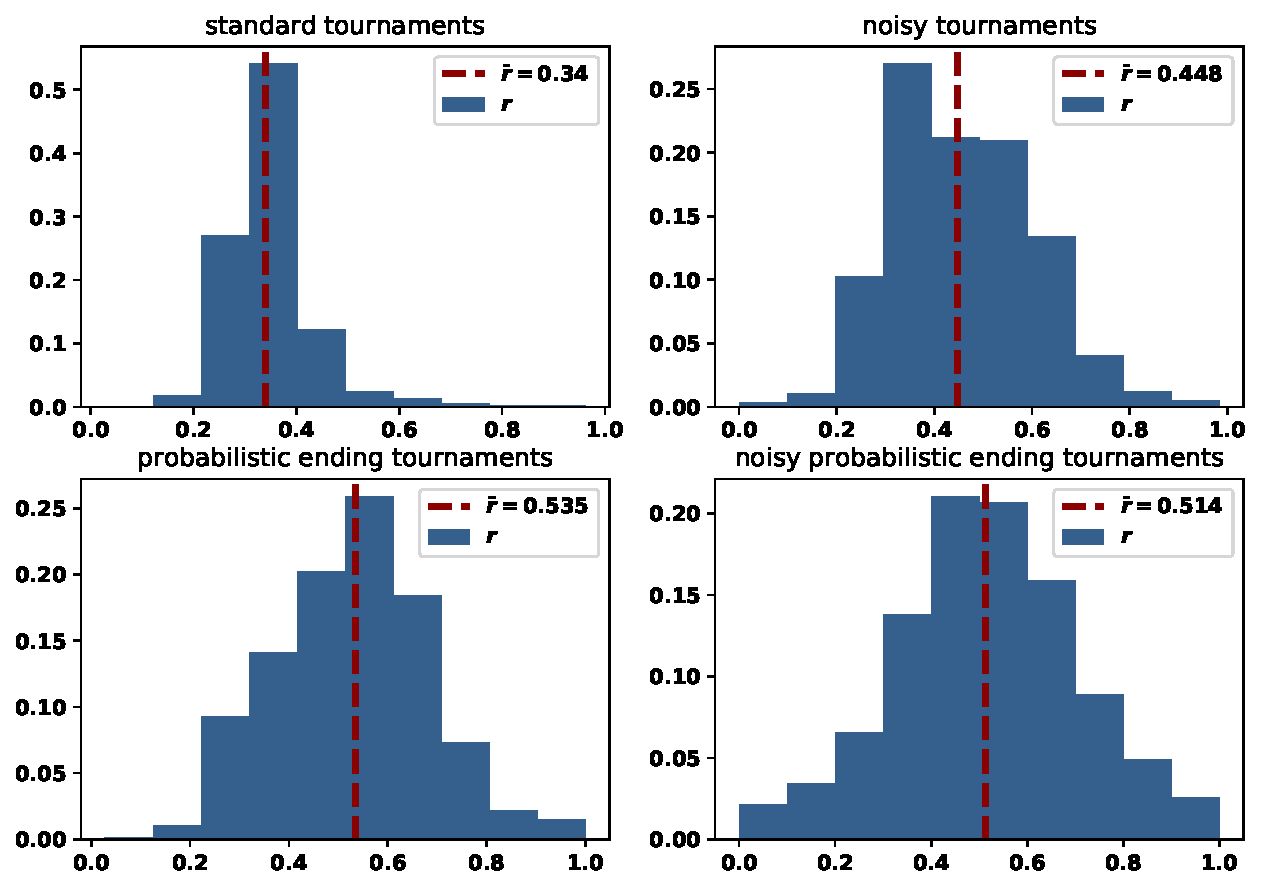
\includegraphics[width=.8\textwidth]{../images/tit_for_tat_r_distributions.pdf}
    \caption{TFT's $r$ distribution in tournaments. Lower values of \(r\)
    correspond to better performances. The best performance
    of the strategy has been in standard tournaments where it achieved a $\bar{r}$
    of 0.34.}
    \label{fig:tit_for_tat_r_distribution}
\end{figure}

The top 15 strategies for each tournament type based on \(\bar{r}\) are given in
Table~\ref{table:top_performances}. The data collection process was designed such
that the probabilities of noise and ending of the match varied between 0 and
1. However, commonly used values for these probabilities are values less than 0.1.
Thus,
Table~\ref{table:top_performances} also includes the top 15 strategies in noisy
tournaments with \(p_n < 0.1\) and probabilistic ending tournaments with \(p_e <
0.1\).

\newcolumntype{g}{>{\columncolor{Gray}}l}
\begin{table}[!htbp]
    \begin{center}
    \resizebox{\textwidth}{!}{
        \begin{tabular}{lggllggllr}
\toprule
& \multicolumn{2}{g}{Standard} & \multicolumn{2}{c}{Noisy} & \multicolumn{2}{g}{Probabilistic ending} &  \multicolumn{2}{c}{Noisy probabilistic ending} \\
\midrule
& Name & $\bar{r}$ &                 Name & $\bar{r}$ &               Name & $\bar{r}$ &                 Name & $\bar{r}$ \\
\midrule
1 &           Evolved HMM 5 &   0.00667 &               Grumpy &    0.1402 &          Fortress4 &   0.01266 &           Alternator &    0.3037 \\
2 &          Evolved FSM 16 &   0.00995 &                  $e$ &   0.19388 &           Defector &   0.01429 &               $\phi$ &   0.30978 \\
3 &    EvolvedLookerUp2 2 2 &   0.01064 &       Tit For 2 Tats &    0.2069 &  Better and Better &   0.01587 &                  $e$ &    0.3125 \\
4 & Evolved FSM 16 Noise 05 &   0.01667 &         Cycle Hunter &   0.21538 &    Tricky Defector &   0.01875 &                $\pi$ &   0.31686 \\
5 &       PSO Gambler 2 2 2 &   0.02143 &       Risky QLearner &   0.22222 &          Fortress3 &   0.02174 &    Limited Retaliate &   0.35263 \\
6 &             Evolved ANN &   0.02878 &          Retaliate 3 &   0.22887 &     Gradual Killer &   0.02532 &     Anti Tit For Tat &   0.35431 \\
7 &           Evolved ANN 5 &    0.0339 &        Cycler CCCCCD &   0.23507 &         Aggravater &   0.02778 &          Retaliate 3 &   0.35563 \\
8 &       PSO Gambler 1 1 1 &   0.03704 &          Retaliate 2 &   0.23913 &             Raider &   0.03077 &  Limited Retaliate 3 &   0.35563 \\
9 &           Evolved FSM 4 &   0.04891 &      Defector Hunter &   0.24038 &         Cycler DDC &   0.04545 &            Retaliate &   0.35714 \\
10 &        PSO Gambler Mem1 &   0.05036 &            Retaliate &   0.24177 &        Hard Prober &   0.05128 &          Retaliate 2 &   0.35767 \\
11 &                Winner12 &   0.06011 &  Hard Tit For 2 Tats &      0.25 &         SolutionB1 &   0.06024 &  Limited Retaliate 2 &   0.36134 \\
12 &            Fool Me Once &    0.0614 &             ShortMem &   0.25286 &      Meta Minority &   0.06077 &             Hopeless &   0.36842 \\
13 &                     DBS &   0.07143 &  Limited Retaliate 3 &   0.25316 &              Bully &   0.06081 &    Arrogant QLearner &   0.40651 \\
14 &           DoubleCrosser &     0.072 &    Limited Retaliate &   0.25706 &    Fool Me Forever &    0.0708 &    Cautious QLearner &   0.40909 \\
15 &             BackStabber &   0.07519 &                $\pi$ &   0.25801 &             EasyGo &   0.07101 &      Fool Me Forever &   0.41764 \\
\bottomrule
    \end{tabular}
    
    }
\end{center}
\caption{Top performances for each tournament type based on $\bar{r}$. The
results of each type are based on 11420 unique tournaments. The
results for noisy tournaments with \(p_n < 0.1\) are based on 1151 tournaments,
and for probabilistic ending tournaments with \(p_e < 0.1\) on 1139. The top
ranks indicate that trained strategies perform well in a variety of
environments, but so do simple deterministic strategies. The normalised medians
are close to 0 for most environments, except environments with noise not
restricted to 0.1 regardless of the number of turns. Noisy and noisy probabilistic
ending tournaments have the highest medians.}
\label{table:top_performances}
\end{table}

The \(r\) distributions for the top ranked strategies of Table~\ref{table:top_performances}
are given by Figure~\ref{fig:r_distributions}.

\begin{figure*}[!htbp]
    \centering
    \begin{subfigure}{0.485\textwidth}
        \centering
        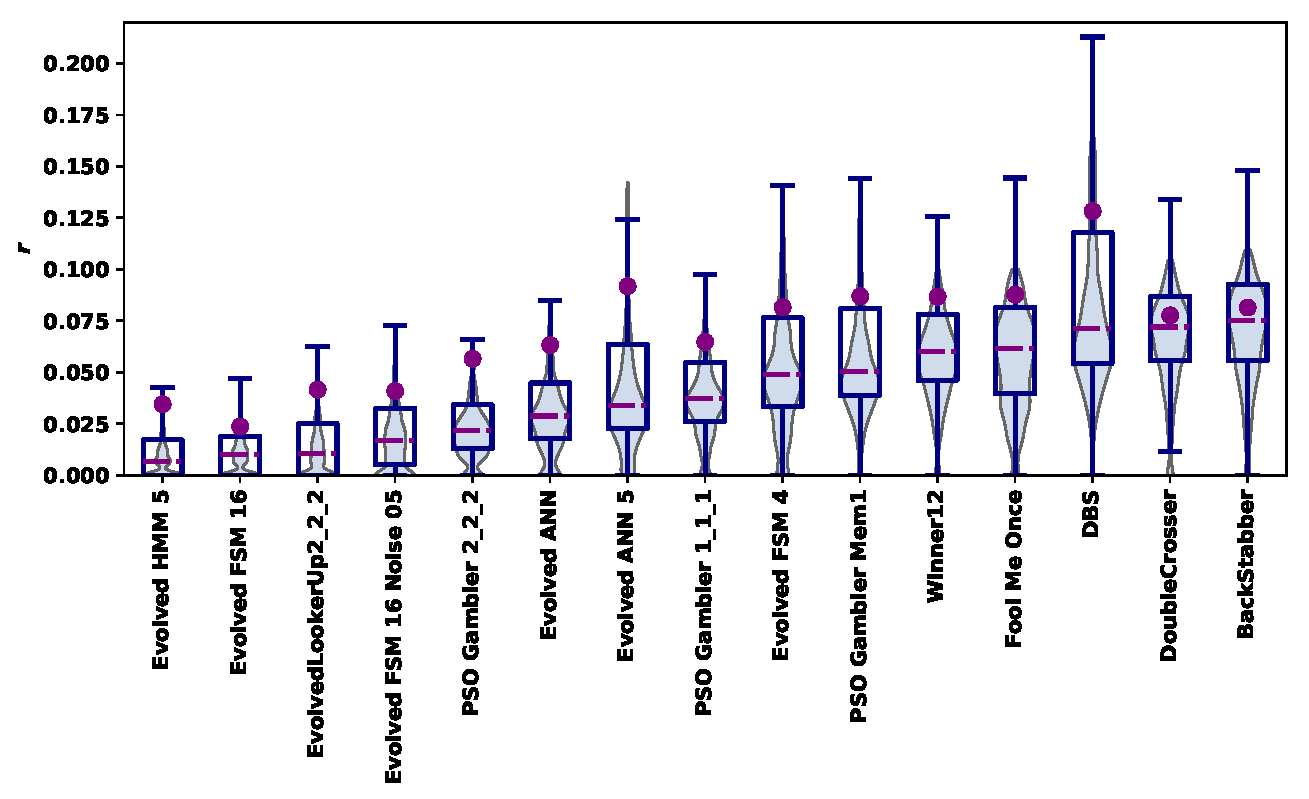
\includegraphics[width=\textwidth]{../images/r_distribution_standard.pdf}
        \caption{$r$ distributions of top 15 strategies in standard tournaments.}\label{fig:std_results}
    \end{subfigure}
    \hfill
    \begin{subfigure}{0.485\textwidth}
        \centering
        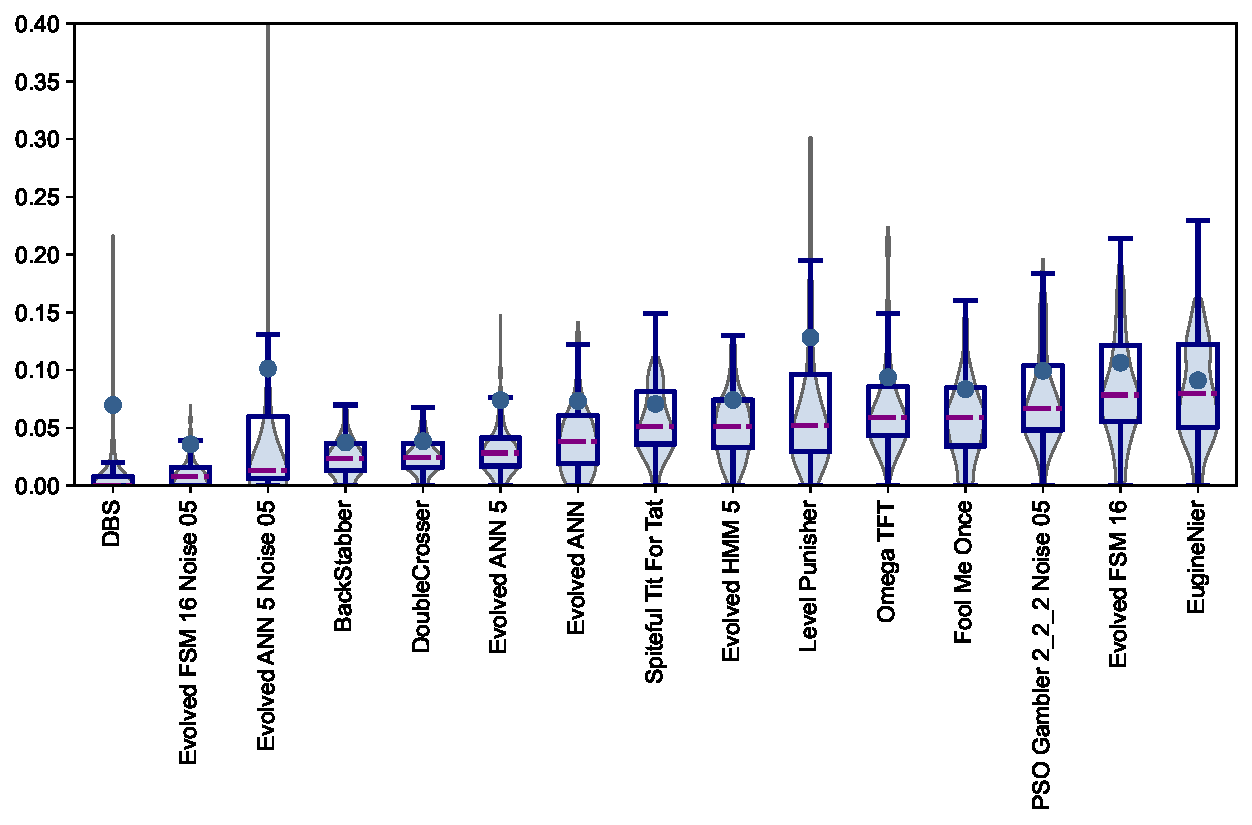
\includegraphics[width=\textwidth]{../images/r_distribution_noise_subset.pdf}
        \caption{$r$ distributions of top 15 strategies in noisy tournaments with \(p_n < 0.1\).}\label{fig:noise_subset_results}
    \end{subfigure}
    \vskip\baselineskip
    \begin{subfigure}{0.485\textwidth}
        \centering
        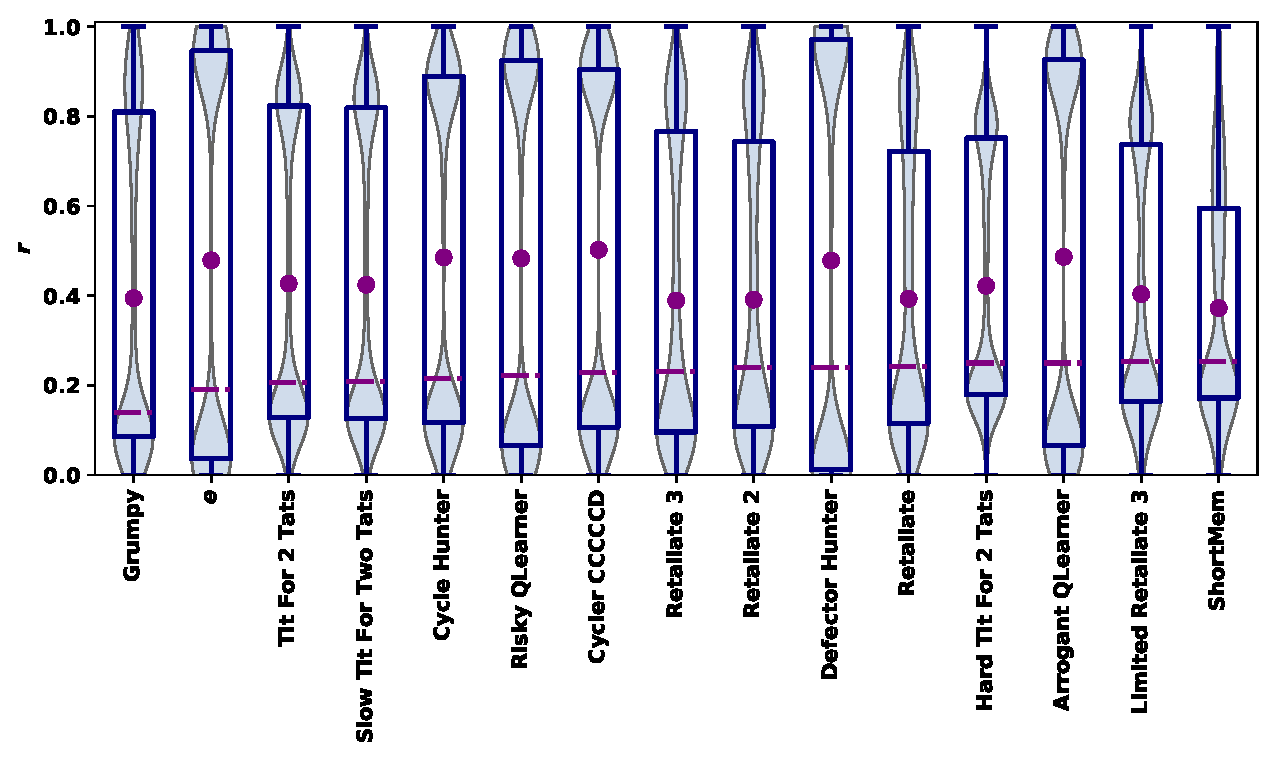
\includegraphics[width=\textwidth]{../images/r_distribution_noise.pdf}
        \caption{$r$ distributions of top 15 strategies in noisy tournaments.}\label{fig:noise_results}
    \end{subfigure}
    \quad
    \begin{subfigure}{0.485\textwidth}
        \centering
        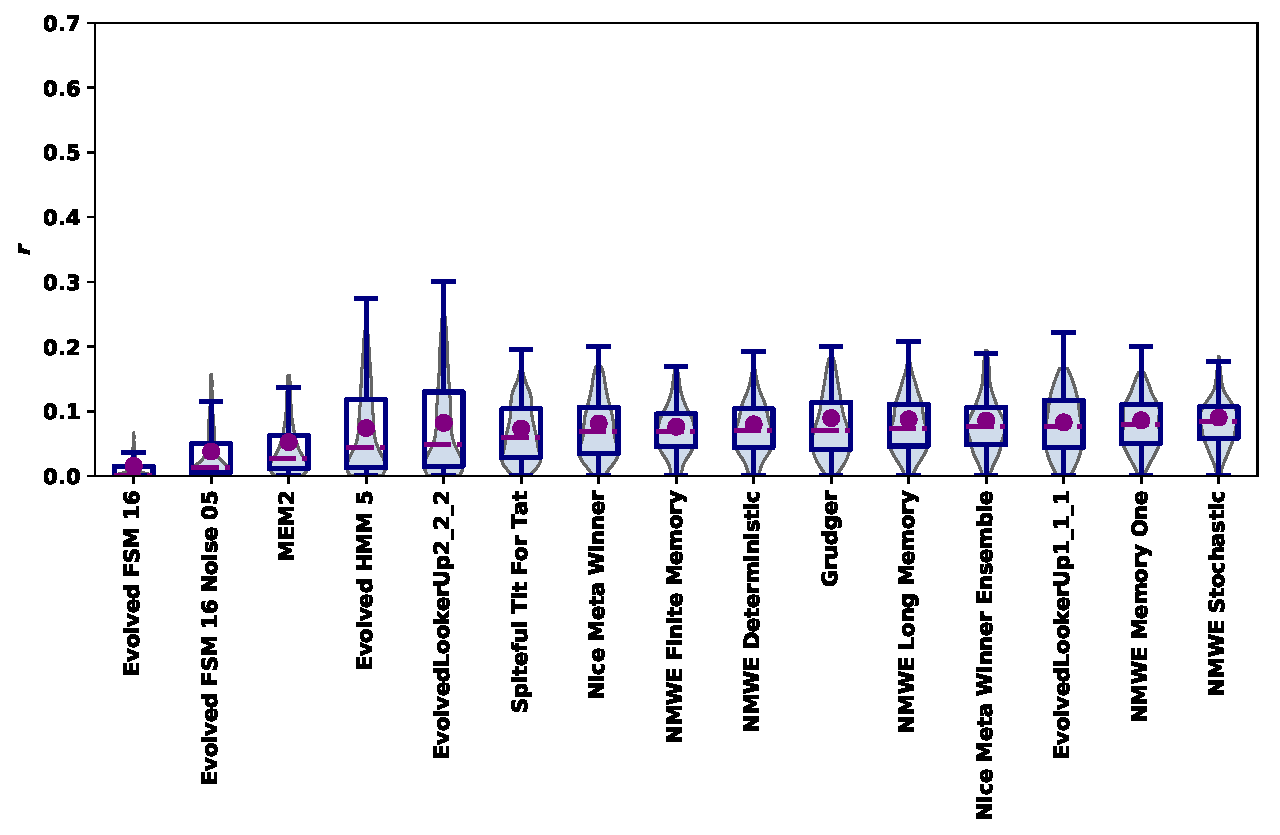
\includegraphics[width=\textwidth]{../images/r_distribution_probend_subset.pdf}
        \caption{\(r\) distributions of top 15 strategies in 1139 probabilistic ending
        tournaments with \(p_e < 0.1\).}
        \label{fig:probend_subset_results}
    \end{subfigure}
    \vskip\baselineskip
    \begin{subfigure}{0.485\textwidth}
        \centering
        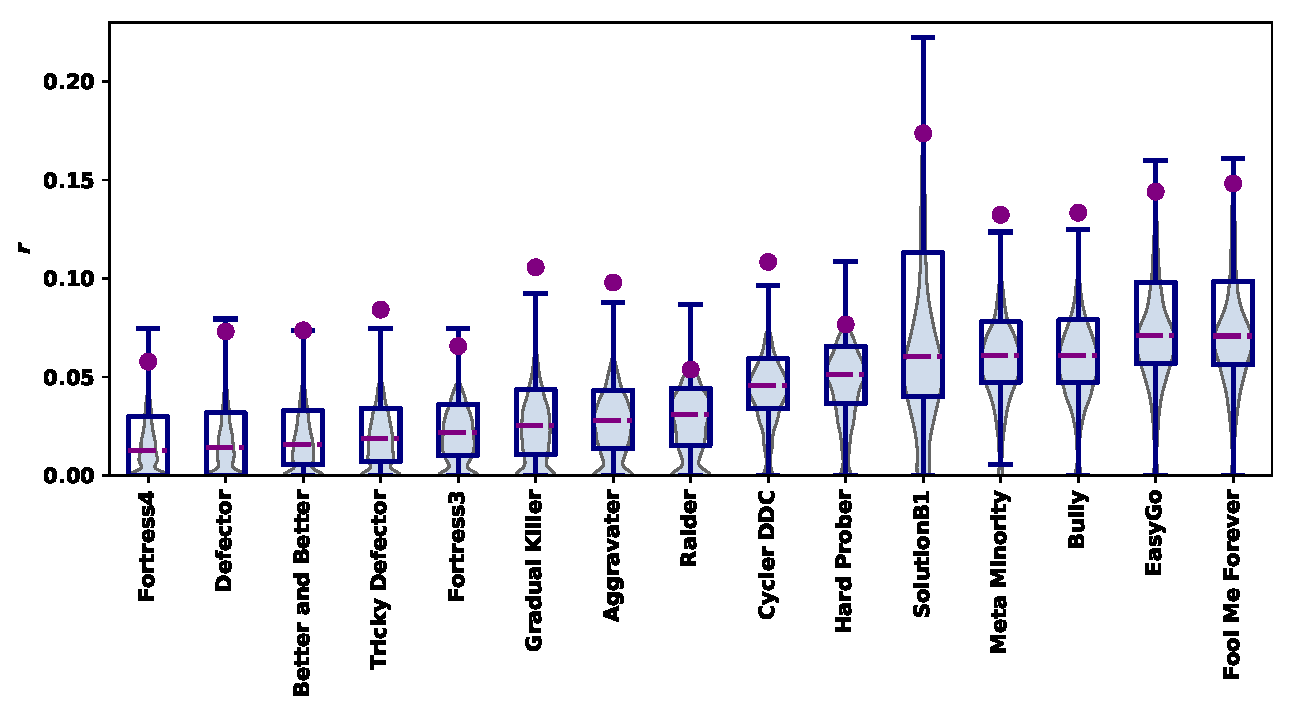
\includegraphics[width=\textwidth]{../images/r_distribution_probend.pdf}
        \caption{$r$ distributions of top 15 strategies in probabilistic ending tournaments.}\label{fig:probend_results}
    \end{subfigure}
    \quad
    \begin{subfigure}{0.485\textwidth}
        \centering
        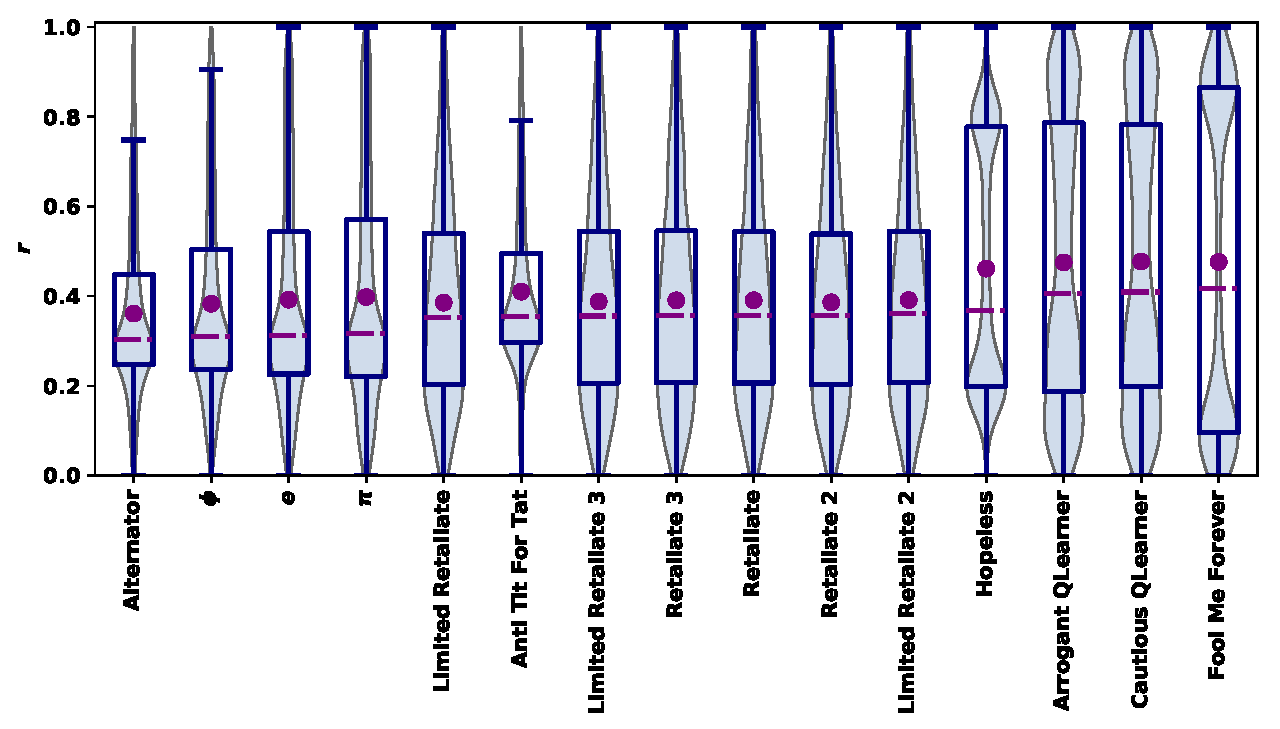
\includegraphics[width=\textwidth]{../images/r_distribution_probend_noise.pdf}
        \caption{$r$ distributions of top 15 strategies in noisy probabilistic ending tournaments.}
        \label{fig:probend_noise_results}
    \end{subfigure}
    \caption{\(r\) distributions of the top 15 strategies in different
    environments. A lower value of \(\bar{r}\) corresponds to a more successful
    performance. A strategy's \(r\) distribution skewed towards zero indicates
    that the strategy ranked highly in most tournaments it participated in. Most
    distributions are skewed towards zero except the distributions with
    unrestricted noise, supporting the conclusions from
    Table~\ref{table:top_performances}.}\label{fig:r_distributions}
\end{figure*}

In standard tournaments 10 out of the 15 top strategies were introduced
in~\cite{Harper2017}. These are strategies based on finite state automata (FSM),
hidden Markov models (HMM), artificial neural networks (ANN), lookup tables
(LookerUp) and stochastic lookup tables (Gambler) that have been trained using
reinforcement learning algorithms (evolutionary and particle swarm algorithms).
They have been trained to perform well against a subset of the strategies
in APL in a standard tournament, thus their performance in the
specific setting was anticipated although still noteworthy given the random
sampling of tournament participants. DoubleCrosser, BackStabber and Fool Me Once, are
strategies not from the literature but from the APL. DoubleCrosser is an extension
of BackStabber and both strategies make use of the number of turns because they are
set to defect on the last two rounds. It should be noted that these
strategies can be characterised as ``cheaters'' because the source code of the strategies
allows them to know the number of turns in a match (unless the match has a probabilistic ending). These strategies were expected to not perform as well in
tournaments where the number of turns is not specified. Finally, Winner
12~\cite{mathieu2017} and DBS~\cite{Au2006} are both from the literature.
DBS is a strategy specifically designed for noisy environments, however, it ranks
highly in standard tournaments as well. Similarly the fourth ranked player,
Evolved FSM 16 Noise 05, was
trained for noisy tournaments yet performs well in standard tournaments.
Figure~\ref{fig:std_results} shows that these strategies typically perform
well in any standard tournament in which they participate.

In the case of noisy tournaments with smaller noise \(p_n < 0.1\) the top
performing strategies
include strategies specifically designed for noisy tournaments. These are DBS,
Evolved FSM 16 Noise 05, Evolved ANN 5 Noise 05, PSO Gambler 2 2 2 Noise 05 and
Omega Tit For Tat~\cite{kendall2007iterated}. Omega TFT, a strategy designed
to break the deadlocking cycles of \(CD\) and \(DC\) that TFT can fall into in noisy
environments, places 10th. The rest of the top ranks are
occupied by strategies which performed well in standard tournaments and
deterministic strategies such as Spiteful Tit For Tat~\cite{prison}, Level
Punisher~\cite{Eckhart2015}, Eugine Nier~\cite{lesswrong}.

In contrast, the performance of the top ranked strategies in noisy environments
when \(p_n\in [0, 1]\) is bimodal. The top strategies include strategies which
decide their actions based on the cooperation to defection ratio, such as
ShortMem~\cite{Andre2013}, Grumpy~\cite{axelrodproject} and
e~\cite{axelrodproject}, and the Retaliate strategies which are designed to
defect if the opponent has tricked them more often than a given percentage of the times that
they have done the same. The bimodality of the \(r\) distributions is explained
by Figure~\ref{fig:effect_of_noise} which demonstrates that the top 6 strategies
were highly ranked due to the their performance in tournaments with \(p_n>0.5\),
and that in tournaments with \(p_n<0.5\) they
performed poorly. At a noisy level of \(0.5\) or greater, mostly cooperative strategies
become mostly defectors and vice versa.

\begin{figure}[!htbp]
    \centering
    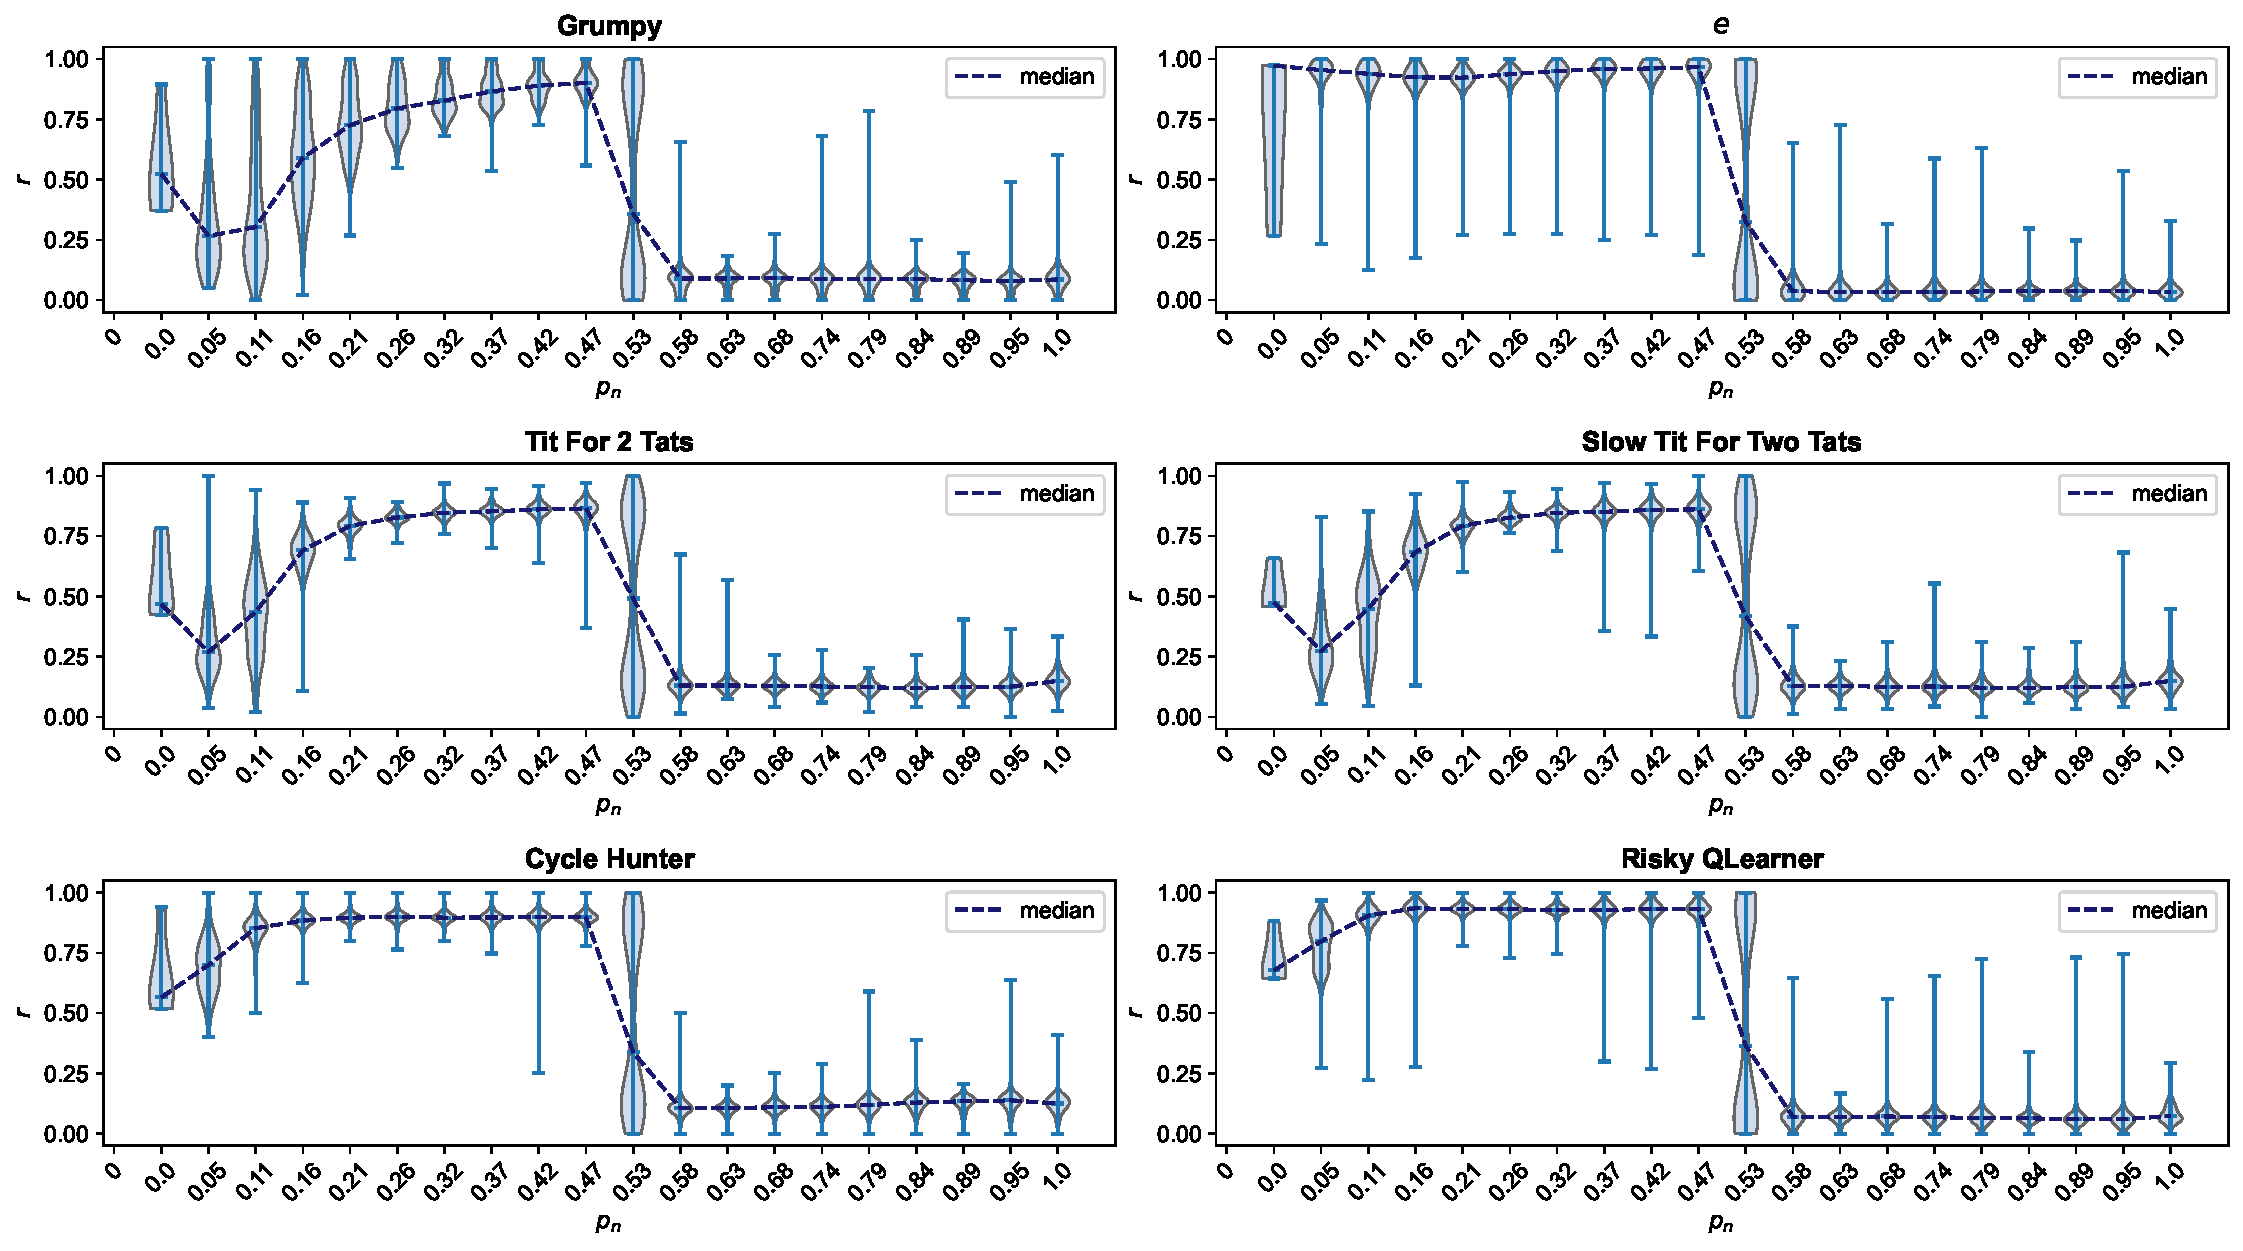
\includegraphics[width=.92\textwidth]{../images/noise_effect.pdf}
    \caption{Normalised rank \(r\) distributions for top 6 strategies in noisy tournaments over
    the probability of noisy ($p_n$).}
    \label{fig:effect_of_noise}
\end{figure}

The most effective strategies in probabilistic ending
tournaments with \(p_e< 0.1\) are a series of ensemble Meta strategies, trained strategies
which performed well
in standard tournaments, and Grudger~\cite{axelrodproject} and Spiteful Tit for
Tat~\cite{prison}. The Meta strategies~\cite{axelrodproject} utilize a team of
strategies and aggregate the potential actions of the team members into a single action
in various ways. Figure~\ref{fig:probend_subset_results} indicates that these strategies
performed well in any probabilistic ending tournament.

In probabilistic ending tournaments with \(p_e \in [0, 1]\) the top ranks are
mostly occupied by defecting strategies such as Better and Better, Gradual
Killer, Hard Prober (all from~\cite{axelrodproject}), Bully (Reverse Tit For
Tat)~\cite{Nachbar1992} and Defector, and a series of strategies based on finite
state automata introduced by Daniel Ashlock and Wendy Ashlock: Fortress 3,
Fortress 4 (both introduced in~\cite{Ashlock2006}), Raider~\cite{Ashlock2014}
and Solution B1~\cite{Ashlock2014}. The success of defecting strategies in
probabilistic ending tournaments is due to larger values of
\(p_e\) which lead to shorter matches (the expected number of rounds is \(1 / p_e\)), so the
impact of the PD being iterated is subdued. This is captured by the Folk
Theorem~\cite{Fudenberg2009} as defecting strategies do better when the likelihood
of the game ending in the next turn increases.
This is demonstrated by Figure~\ref{fig:effect_of_probend}, which gives the
distributions of \(r\) for the top 6 strategies in probabilistic ending tournaments
over \(p_e\).

\begin{figure}[!htbp]
    \centering
    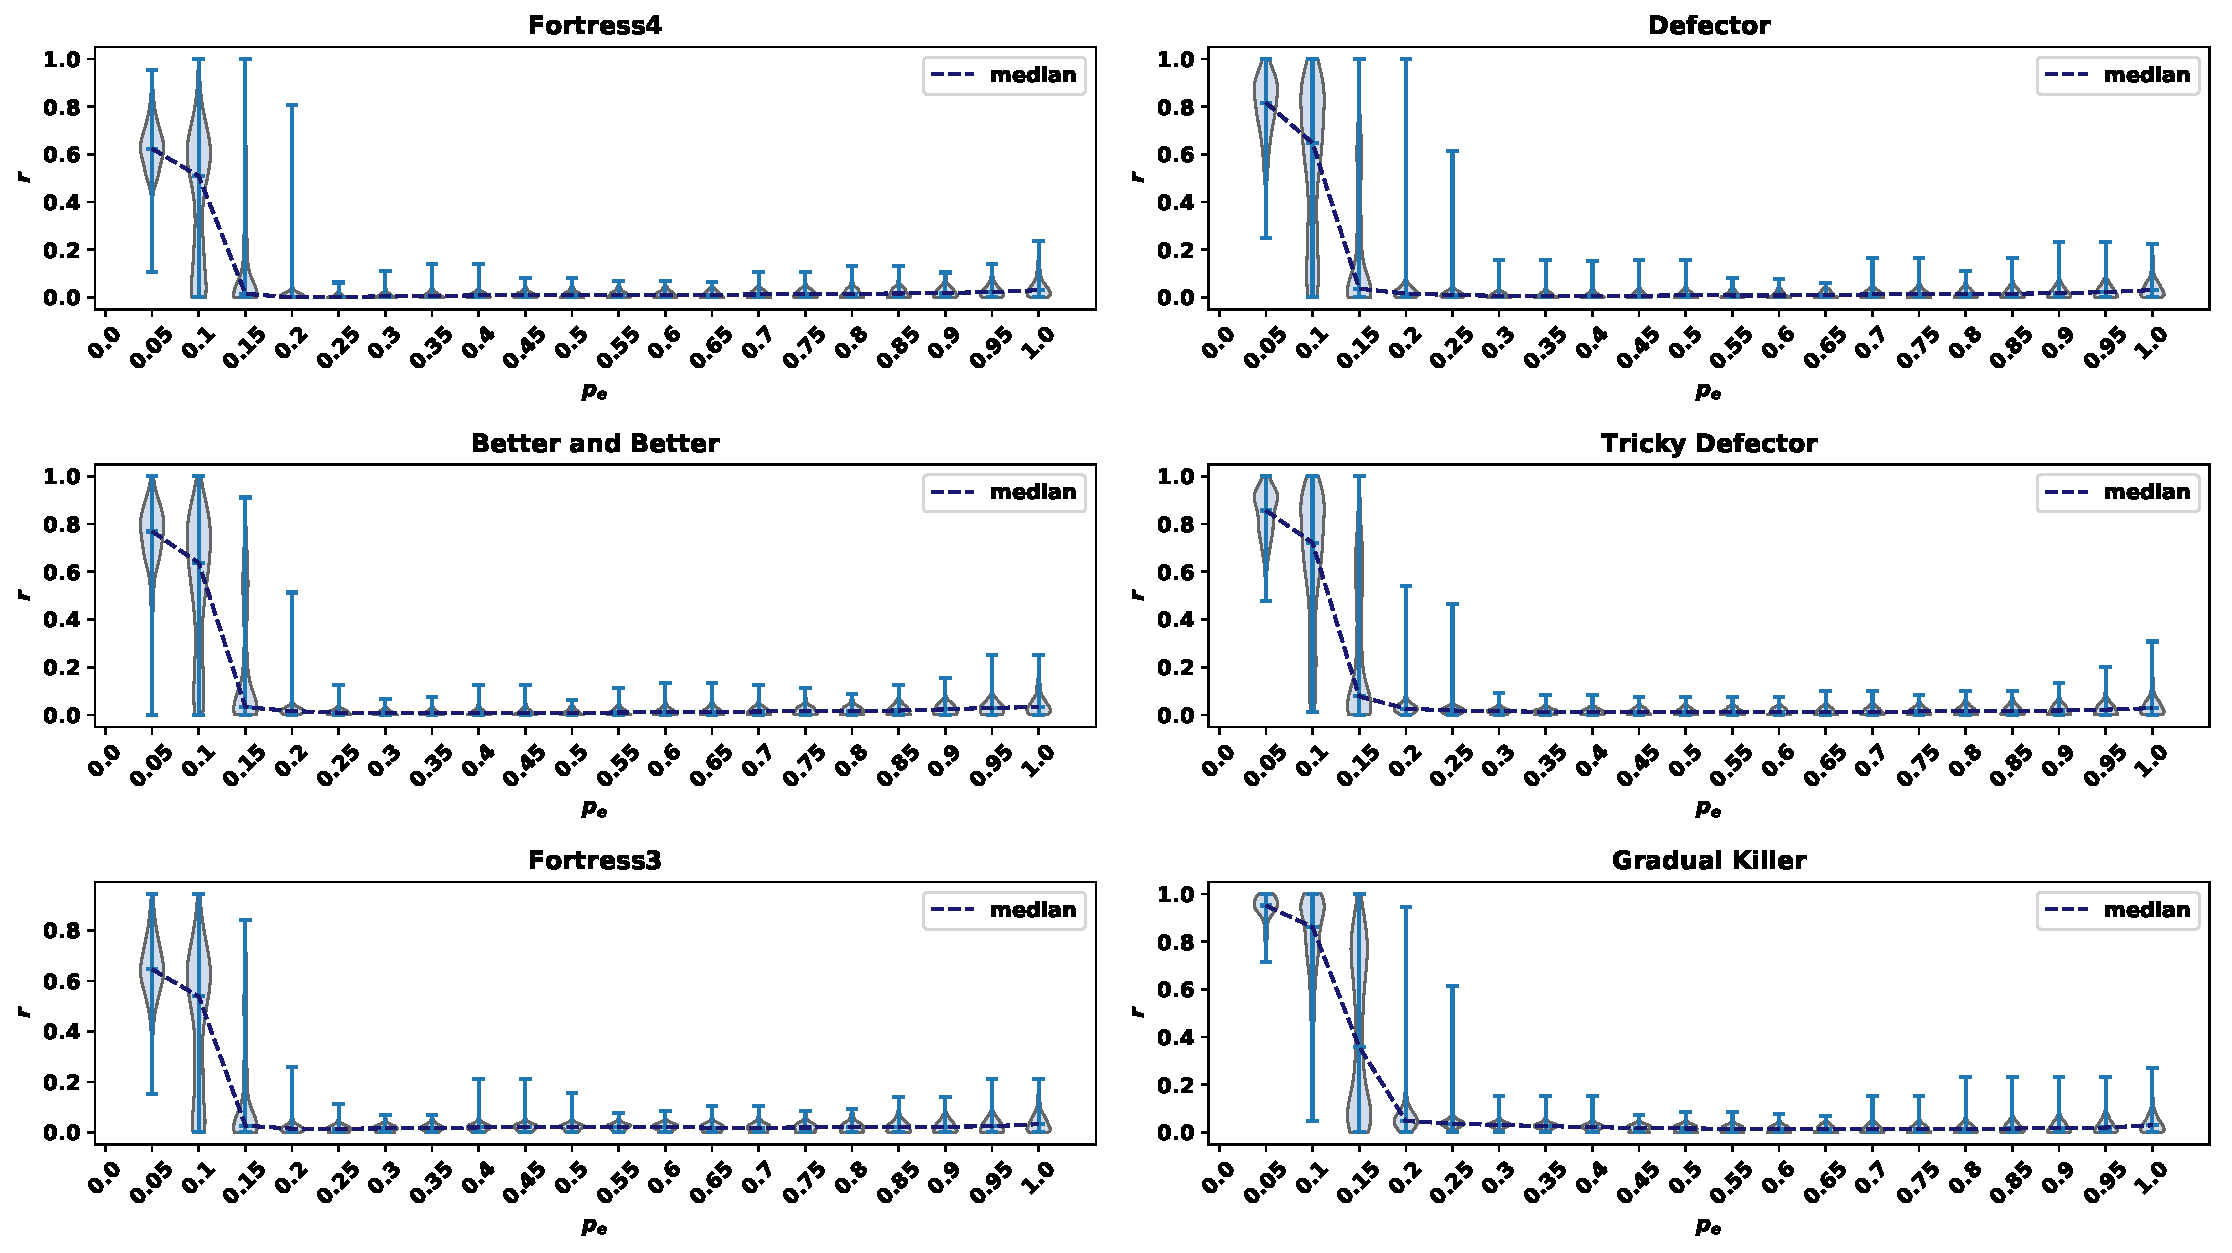
\includegraphics[width=.92\textwidth]{../images/folk_theorem.pdf}
    \caption{Normalised rank \(r\) distributions for top 6 strategies in probabilistic ending tournaments
    over $p_e$. The 6 strategies start of with a high median rank,
    however, their ranked decreased as the the probability of the game ending
    increased and at the point of \(p_e = 0.1\).}
    \label{fig:effect_of_probend}
\end{figure}

The top performances in tournaments with both noise and a probabilistic ending
and the top performances over the entire data set have the largest median values
compared to the top rank strategies of the other tournament types,
Figure~\ref{fig:probend_noise_results} and Figure~\ref{fig:overall_results}. The
\(\bar{r}\) for the top strategy is approximately at 0.3, indicating that the
most successful strategy can on average just place in the top 30\% of the
competition.

\begin{table}[!htbp]
    \centering
    \resizebox{.30\textwidth}{!}{
    \begin{tabular}{lr}
\toprule
{} &  Normalized\_Rank \\
Name                    &                  \\
\midrule
Evolved FSM 16          &            0.018 \\
Evolved HMM 5           &            0.019 \\
Evolved FSM 16 Noise 05 &            0.025 \\
EvolvedLookerUp2\_2\_2    &            0.028 \\
Evolved ANN             &            0.037 \\
PSO Gambler 2\_2\_2       &            0.040 \\
Evolved ANN 5           &            0.046 \\
PSO Gambler 1\_1\_1       &            0.061 \\
Fool Me Once            &            0.067 \\
Evolved FSM 4           &            0.075 \\
DoubleCrosser           &            0.079 \\
Winner12                &            0.081 \\
BackStabber             &            0.082 \\
DBS                     &            0.086 \\
PSO Gambler Mem1        &            0.089 \\
\bottomrule
\end{tabular}
}
    \caption{Top performances over all the tournaments. The top ranks include
    strategies that have been previously mentioned. The set of Retaliate
    strategies occupy the top spots followed by BackStabber and DoubleCrosser.
    The distributions of the Retaliate strategies have no statistical
    difference. PSO Gambler and Evolved HMM 5 are trained strategies introduced
    in~\cite{Harper2017} and Nice Meta Winner and NMWE Memory One are strategies
    based on teams. Grudger is a strategy from R. Axelrod's original tournament and
    Forgetful Fool Me Once is based on the same approach as
    Grudger.}\label{table:overall_results}
\end{table}

\begin{figure}[!htbp]
        \centering
        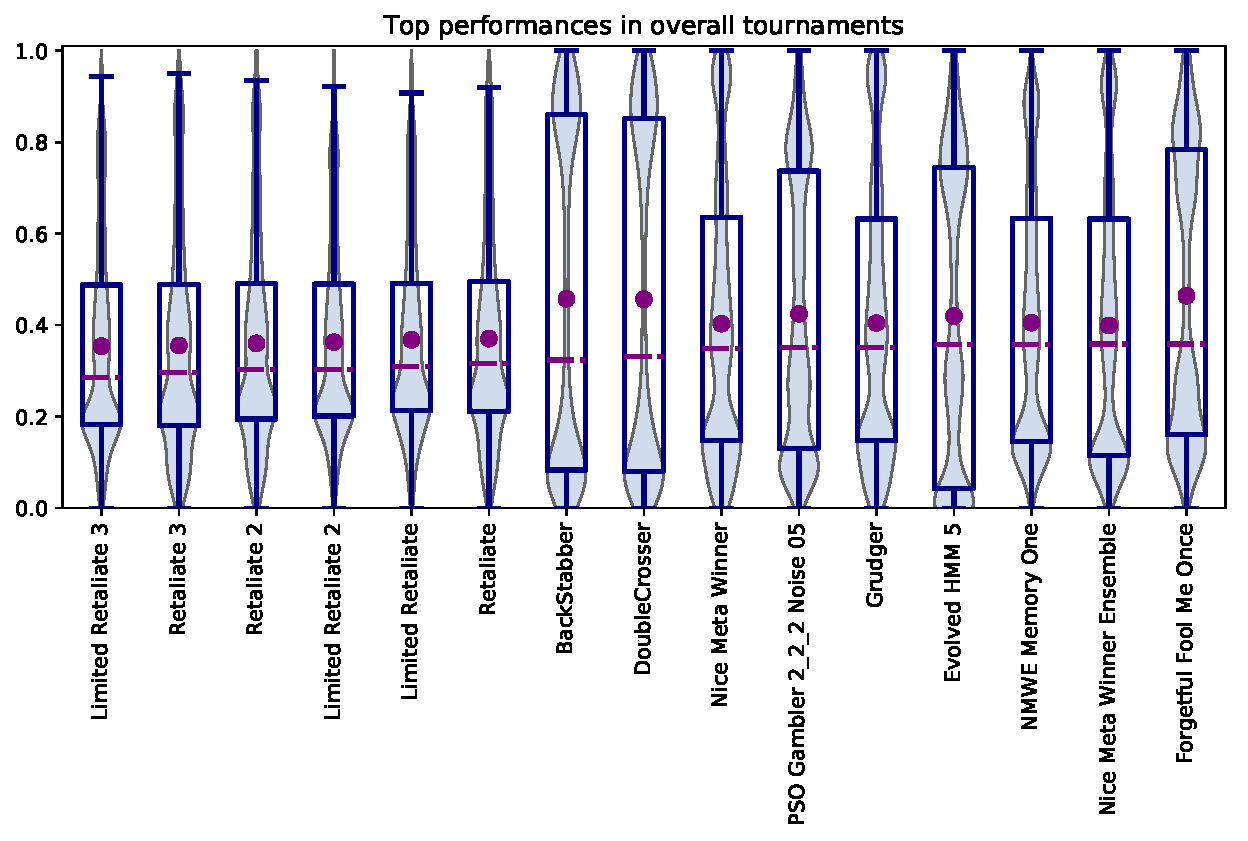
\includegraphics[width=.65\textwidth]{../images/performance_merged.pdf}
        \caption{Normalised rank \(r\) distributions for best performed strategies in the data set~\cite{data}.
        A lower value of \(\bar{r}\) corresponds to a more successful
        performance.}
        \label{fig:overall_results}
\end{figure}

On the whole, the analysis of this manuscript has shown that:

\begin{itemize}
    \item In standard tournaments the dominating strategies were
    strategies that had been trained using reinforcement learning techniques.
    \item In noisy environments where the noise probability strictly less than
    0.1 was considered, the successful strategies were strategies specifically
    designed or trained for noisy environments.
    \item In probabilistic ending tournaments most of the highly ranked
    strategies were defecting strategies and trained finite state automata, all
    by the authors of~\cite{Ashlock2006, Ashlock2014}. These strategies ranked
    high due to their performance in tournaments where the probability of the
    game ending after each turn was bigger than 0.1.
    \item In probabilistic tournaments with \(p_e\) less than 0.1 the highly
    ranked strategies were strategies based on the behaviour of others.
    \item From the collection of strategies considered here,  no strategy can be
    consistently successful in noisy environments, except if the value of noise
    is constrained to less than a 0.1.
\end{itemize}

Though there is not a single strategy that repeatably outranks all others in any
of the distinct tournament types, or even across the tournament types, there
are specific types of strategies have been repeatably ranked in the top ranks.
These have been strategies that have been trained, strategies that retailiate,
and strategies that would adapt their behaviour based on preassigned rules
to achieve the highest outcome. These results contradict some of R. Axelrod's suggestions,
and more specifically, the suggestions `Do not be clever' and `Do not be envious'.
We dig deeper into the crucial strategy features for success in the following section.

\section{Evaluation of performance}\label{section:evaluation_of_performance}

For each strategy, for each tournament we have a variety of features, described in
Table~\ref{table:manual_features}. These features are measures regarding a
strategy's behaviour from the tournaments the strategies competed in as well as
intrinsic properties such as whether a strategy is deterministic or stochastic.

\newcolumntype{g}{>{\columncolor{Gray}}c}
\begin{table}[!htbp]
    \begin{center}
    \resizebox{.99\textwidth}{!}{
    \begin{tabular}{gcgcgc}
    \toprule
    feature & feature explanation &  source & value type & min value & max value \\
    \midrule
stochastic  &  If a strategy is stochastic & strategy classifier from APL & boolean  & Na &  Na \\
makes use of game &  If a strategy makes used of the game information & strategy classifier from APL & boolean  & Na &  Na \\
makes use of length &  If a strategy makes used of the number of turns & strategy classifier from APL & boolean  & Na &  Na \\
memory usage &  The memory size of a strategy divided by the number of turns & memory size from APL & float & 0 &  1 \\
SSE & A measure of how far a strategy is from ZD behaviour & method described in~\cite{Knight2019} & float & 0 & 1 \\
max cooperating rate $(C_{\text{max}})$  & The biggest cooperating rate in a given tournament  & result summary  & float & 0 & 1\\
min cooperating rate $(C_{\text{min}})$ & The smallest cooperating rate in a given tournament  & result summary  & float & 0 & 1\\
median cooperating rate $(C_{\text{median}})$ & The median cooperating rate in a given tournament  & result summary  & float & 0 & 1\\
mean cooperating rate $(C_{\text{mean}})$ & The mean cooperating rate in a given tournament  & result summary  & float & 0 & 1 \\
$C_r$ / $C_{\text{max}}$ & A strategy's cooperating rate divided by the maximum & result summary  & float & 0 & 1 \\
$C_{\text{min}}$ / $C_r$ & A strategy's cooperating rate divided by the minimum & result summary  & float & 0 & 1 \\
$C_r$ / $C_{\text{median}}$ & A strategy's cooperating rate divided by the median  & result summary  & float & 0 & 1\\
$C_r$ / $C_{\text{mean}}$ & A strategy's cooperating rate divided by the mean & result summary  & float & 0 & 1 \\
$C_r$ & The cooperating ratio of a strategy & result summary  & float & 0 & 1 \\
$CC$ to $C$ rate & The probability a strategy will cooperate after a mutual cooperation & result summary  & float & 0 & 1\\
$CD$ to $C$ rate & The probability a strategy will cooperate after being betrayed by the opponent & result summary  & float & 0 & 1 \\
$DC$ to $C$ rate & The probability a strategy will cooperate after betraying the opponent & result summary  & float & 0 & 1 \\
$DD$ to $C$ rate & The probability a strategy will cooperate after a mutual defection & result summary  & float & 0 & 1 \\
$p_n$ & The probability of a player's action being flip at each interaction & trial summary & float & 0 & 1 \\
$n$ & The number of turns & trial summary & integer & 1 & 200 \\
$p_e$ & The probability of a match ending in the next turn & trial summary & float & 0 & 1 \\
$N$ & The number of strategies in the tournament & trial summary & integer & 3 & 195 \\
$k$ & The number of repetitions of a given tournament & trial summary & integer & 10 & 100 \\
    \bottomrule
        \end{tabular}}
    \end{center}
    \caption{The features which are included in the performance evaluation
    analysis. Stochastic, makes use of length and makes use of game are APL
    classifiers that determine whether a strategy is stochastic or deterministic,
    whether it makes use of the number of turns or the game's payoffs. The
    memory usage is calculated as the number of turns the strategy considers to
    make an action (which is specified in the APL) divided by the number of
    turns. The SSE (introduced in~\cite{Knight2019}) shows how close a strategy
    is to behaving as a ZDs, and subsequently, in an extortionate way. The
    method identifies the ZDs closest to a given strategy and calculates the
    algebraic distance between them as the sum of squared error (SSE). A SSE value of 1 indicates
    no extortionate behaviour at all whereas a value of 0 indicates that a
    strategy is behaving as a ZDs. The rest of the features considered are the $CC$
    to $C$, $CD$ to $C$, $DC$ to $C$, and $DD$ to $C$ rates as well as
    cooperating ratio of a strategy, the minimum (\(C_{min}\)), maximum
    (\(C_{max}\)), mean (\(C_{mean}\)) and median (\(C_{median}\)) cooperating
    ratios of each tournament.}
    \label{table:manual_features}
\end{table}

The memory usage of strategies is the number of
rounds of play used by the strategy divided by the number of turns in each match.
For example, Winner12 uses the previous two rounds of play, and if participating
in a match with 100 turns its memory usage would be 2/100.
For strategies with an infinite memory size, for example Evolved
FSM 16 Noise 05, memory usage is equal to 1.
Note that for tournaments with a probabilistic
ending the number of turns was not collected, so the memory usage feature is not
used for probabilistic ending tournaments.

The correlation coefficients between the features of
Table~\ref{table:manual_features} the median score and the median normalised
rank are given by Table~\ref{table:correlations}. The correlation coefficients
between all features of Table~\ref{table:manual_features} have been calculated
and a graphical representation can be found in the
Appendix~\ref{app:correlations}.

\newcolumntype{g}{>{\columncolor{Gray}}c}
\begin{table}[!htbp]
    \begin{center}
    \resizebox{.9\textwidth}{!}{
        \begin{tabular}{lggccggccggg}
    \toprule
    &  \multicolumn{2}{g}{Standard} & \multicolumn{2}{c}{Noisy} & \multicolumn{2}{g}{Probabilistic ending} &  \multicolumn{2}{c}{Noisy probabilistic ending} &  \multicolumn{2}{g}{Overall} \\
\midrule
{} &  $r$ &  median score &  $r$ &  median score &  $r$ &  median score &  $r$ &  median score &  $r$ &  median score\\
\midrule
$CC$ to $C$ rate     & -0.501 &  0.501 &   0.414 &  -0.504 &   0.408 &  -0.323 &   0.260 &   0.022 &  -0.501 &  0.501 \\
$CD$ to $C$ rate     &  0.226 & -0.199 &   0.456 &  -0.330 &   0.320 &  -0.017 &   0.205 &  -0.220 &   0.226 & -0.199 \\
$C_r$                & -0.323 &  0.384 &   0.711 &  -0.678 &   0.714 &  -0.832 &   0.579 &  -0.135 &  -0.323 &  0.384 \\
$C_r$ / $C_{max}$    & -0.323 &  0.381 &   0.616 &  -0.551 &   0.714 &  -0.833 &   0.536 &  -0.116 &  -0.323 &  0.381 \\
$C_r$ / $C_{mean}$   & -0.331 &  0.358 &   0.731 &  -0.740 &   0.721 &  -0.861 &   0.649 &  -0.621 &  -0.331 &  0.358 \\
$C_r$ / $C_{median}$ & -0.331 &  0.353 &   0.652 &  -0.669 &   0.712 &  -0.852 &   0.330 &  -0.466 &  -0.331 &  0.353 \\
$C_r$ / $C_{min}$    &  0.109 & -0.080 &  -0.358 &   0.250 &  -0.134 &   0.150 &  -0.368 &   0.113 &   0.109 & -0.080 \\
$C_{max}$            & -0.000 &  0.049 &   0.000 &   0.023 &  -0.000 &   0.046 &   0.000 &  -0.004 &  -0.000 &  0.049 \\
$C_{mean}$           & -0.000 &  0.229 &  -0.000 &   0.271 &   0.000 &   0.200 &   0.000 &   0.690 &  -0.000 &  0.229 \\
$C_{median}$         &  0.000 &  0.209 &  -0.000 &   0.240 &  -0.000 &   0.187 &  -0.000 &   0.673 &   0.000 &  0.209 \\
$C_{min}$            &  0.000 &  0.084 &   0.000 &  -0.017 &  -0.000 &   0.007 &  -0.000 &   0.041 &   0.000 &  0.084 \\
$DC$ to $C$ rate     &  0.127 & -0.100 &   0.509 &  -0.504 &  -0.018 &   0.033 &   0.341 &  -0.016 &   0.127 & -0.100 \\
$DD$ to $C$ rate     &  0.412 & -0.396 &   0.533 &  -0.436 &  -0.103 &   0.176 &   0.378 &  -0.263 &   0.412 & -0.396 \\
$N$                  &  0.000 & -0.009 &  -0.000 &   0.002 &  -0.000 &   0.003 &  -0.000 &   0.001 &   0.000 & -0.009 \\
$k$                  &  0.000 & -0.002 &  -0.000 &   0.003 &  -0.000 &   0.001 &  -0.000 &  -0.008 &   0.000 & -0.002 \\
$n$                  &  0.000 & -0.125 &  -0.000 &  -0.024 &       - &       - &       - &       - &   0.000 & -0.125 \\
$p_e$                &      - &      - &        - &     - &    0.000 &   0.165 &   0.000 &  -0.058 &  -0.001 &  0.001 \\
$p_n$                &      - &      - &  -0.000 &   0.207 &       - &       - &  -0.000 &  -0.650 &   0.002 & -0.000 \\
Make use of game     & -0.003 & -0.022 &   0.025 &  -0.082 &  -0.053 &  -0.108 &   0.013 &  -0.016 &  -0.003 & -0.022 \\
Make use of length   & -0.158 &  0.124 &   0.005 &  -0.123 &  -0.025 &  -0.090 &   0.014 &  -0.016 &  -0.154 &  0.117 \\
SSE                  &  0.473 & -0.452 &   0.463 &  -0.337 &  -0.156 &   0.223 &   0.305 &  -0.259 &   0.473 & -0.452 \\
memory usage         & -0.082 &  0.095 &  -0.007 &  -0.017 &       - &     - &     - &           - &  -0.084 &  0.095 \\
stochastic           &  0.006 & -0.024 &   0.022 &  -0.026 &   0.002 &  -0.130 &   0.021 &  -0.013 &   0.006 & -0.024 \\
\bottomrule
\end{tabular}

    }
\end{center}
\caption{Correlations between the features of Table~\ref{table:manual_features}
and the normalised rank and the median score.}\label{table:correlations}
\end{table}

In standard tournaments the features $CC$ to $C$, $C_r$, $C_r / C_{\text{max}}$
and the cooperating ratio compared to $C_{\text{median}}$ and $C_{\text{mean}}$
have a moderately negative effect on the normalised rank (smaller rank is better), and a moderate positive
on the median score. The SSE error and the $DD$ to $C$ rate have the opposite
effects. Thus, in standard tournaments behaving cooperatively corresponds to a
more successful performance. Even though being nice generally pays off
that does not hold against defective strategies. Being more cooperative after a mutual
defection, that is not retaliating, is associated to lesser overall success in terms of normalised rank.
Figure~\ref{fig:rates_of_winners_in_standard_tournaments} confirms that the
winners of standard tournaments always cooperate after a mutual cooperation and
almost always defect after a mutual defection.

\begin{figure}[!htbp]
    \centering
    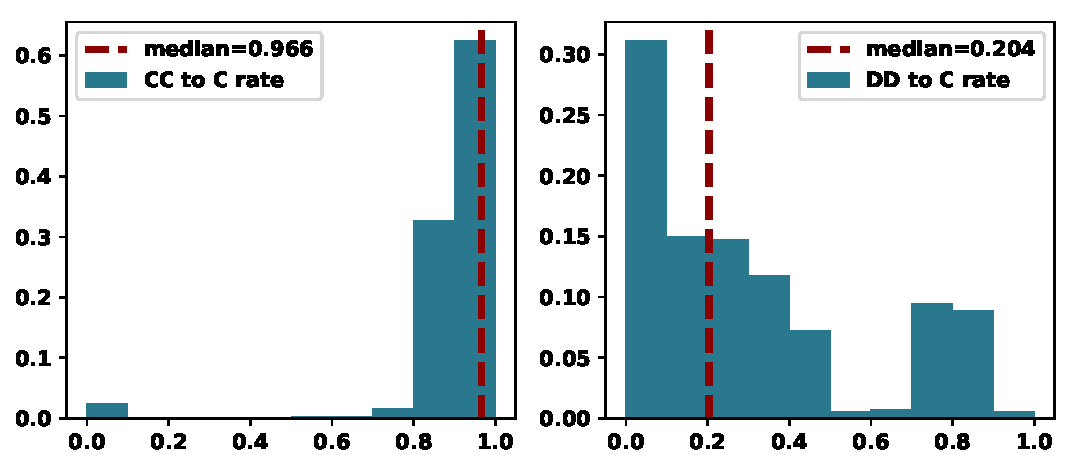
\includegraphics[width=.8\textwidth]{../images/rates_of_winners_in_standard_tournaments.pdf}
    \caption{Distributions of $CC$ to $C$ and $DD$ to $C$ for the winners in
    standard tournaments.}\label{fig:rates_of_winners_in_standard_tournaments}
\end{figure}

Compared to standard tournaments, in both noisy and in probabilistic ending
tournaments the higher the rates of cooperation the lower a strategy's success
and median score. A strategy would want to cooperate less than both
the mean and median cooperator in such settings. In probabilistic ending
tournaments the correlation coefficients have larger values, indicating a
stronger effect. Thus a strategy will be punished more by its cooperative
behaviour in probabilistic ending environments, supporting the results of
Section~\ref{section:evaluation_of_performance}
as well. The distributions of the $C_r$ of the winners in
both tournaments are given by Figure~\ref{fig:c_r_distributions}. It confirms
that the winners in noisy tournaments cooperated less than 35\% of the time
and in probabilistic ending tournaments less than 10\%.
In noisy probabilistic ending tournaments and over all the tournaments' results,
the only features that had a moderate effect are $C_r/C_{\text{mean}},
C_r/C_{\text{max}}$ and $C_r$. In such environments cooperative behaviour
appears to be punished less than in noisy and probabilistic ending
tournaments.


\begin{figure}[!htbp]
    \centering
    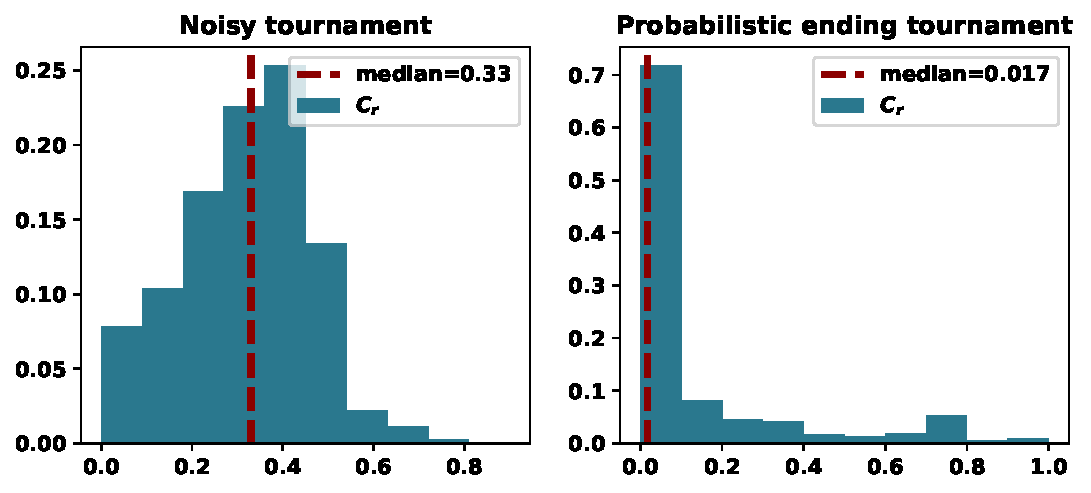
\includegraphics[width=.8\textwidth]{../images/c_r_winners_tournaments.pdf}
    \caption{$C_r$ distributions of the winners in noisy and in probabilistic
    ending tournaments.}\label{fig:c_r_distributions}
\end{figure}

A multivariate linear regression has been fitted to model the relationship between
the features and the normalised rank. Based on the graphical representation of
the correlation matrices given in Appendix~\ref{app:correlations} several of the
features are highly correlated and have been removed
before fitting the linear regression model. The features included are given
by Table~\ref{table:linear_regression} alongside their corresponding \(p\) values
in the distinct tournaments and their regression coefficients.

\newcolumntype{g}{>{\columncolor{Gray}}c}
\begin{table}[h]
    \begin{center}
\resizebox{\textwidth}{!}{
    \begin{tabular}{lggccggcc}
\toprule
& \multicolumn{2}{g}{Standard} & \multicolumn{2}{c}{Noisy} & \multicolumn{2}{g}{Probabilistic ending} & \multicolumn{2}{c}{Noisy probabilistic ending} \\
\midrule
& \multicolumn{2}{c}{\(R\) adjusted: 0.886} & \multicolumn{2}{c}{\(R\) adjusted: 0.912} & \multicolumn{2}{g}{\(R\) adjusted: 0.900} & \multicolumn{2}{c}{\(R\) adjusted: 0.895} \\

{} &  Coefficient &  \(p\)-value &  Coefficient &  \(p\)-value &  Coefficient &  \(p\)-value &  Coefficient &  \(p\)-value\\
\midrule
$CC$ to $C$ rate       & -0.050 &  0.000 & -0.073 &  0.000 &  0.009 &  0.000 &  0.009 &    0.0 \\
$CD$ to $C$ rate       &  0.298 &  0.000 & -0.018 &  0.000 &  0.192 &  0.000 &  0.072 &    0.0 \\
$C_r$                  & -0.701 &  0.000 & -0.959 &  0.000 &  0.348 &  0.000 & -0.383 &    0.0 \\
$C_r$ / $C_{max}$    &  2.587 &  0.000 &  2.389 &  0.000 &  1.679 &  0.000 &  1.348 &    0.0 \\
$C_r$ / $C_{mean}$   & -1.488 &  0.000 & -0.492 &  0.000 & -1.380 &  0.000 & -0.070 &    0.0 \\
$C_r$ / $C_{median}$ & -0.189 &  0.000 &  0.026 &  0.000 &  0.455 &  0.000 & -0.010 &    0.0 \\
$C_r$ / $C_{min}$    &  0.086 &  0.000 & -0.268 &  0.000 &  0.108 &  0.000 & -0.202 &    0.0 \\
$C_{max}$            &  1.961 &  0.000 &  1.544 &  0.000 &  1.411 &  0.000 &  0.780 &    0.0 \\
$C_{mean}$           & -2.538 &  0.000 & -2.369 &  0.000 & -2.578 &  0.000 & -1.192 &    0.0 \\
$C_{median}$         &  0.511 &  0.000 & -0.079 &  0.000 &  0.470 &  0.000 & -0.212 &    0.0 \\
$C_{min}$            & -0.079 &  0.000 & -0.366 &  0.000 & -0.133 &  0.000 & -0.218 &    0.0 \\
$DC$ to $C$ rate       &  0.203 &  0.000 &  0.137 &  0.000 & -0.020 &  0.000 &  0.084 &    0.0 \\
$DD$ to $C$ rate       &  0.092 &  0.000 &  0.293 &  0.000 &  0.088 &  0.000 &  0.248 &    0.0 \\
$N$                    & -0.000 &  0.000 & -0.000 &  0.000 & -0.000 &  0.713 & -0.000 &    0.0 \\
$k$                    &  0.000 &  0.002 &  0.000 &  0.997 &  0.000 &  0.013 &  0.000 &    0.0 \\
$n$                    &  0.000 &  0.000 & -0.000 &  0.000 &    -   &    -   &    -   &    -   \\
$p_e$                  &    -   &    -   &    -   &    -   &  0.004 &  0.125 & -0.052 &    0.0 \\
$p_n$                  &    -   &    -   & -0.059 &  0.000 &    -   &    -   & -0.060 &    0.0 \\
SSE                    &  0.198 &  0.000 & -0.048 &  0.000 & -0.102 &  0.000 & -0.106 &    0.0 \\
memory usage           & -0.008 &  0.000 &  0.000 &  0.250 &    -   &    -   &    -   &    -   \\
\bottomrule
\end{tabular}}
    \end{center}
    \caption{Results of multivariate linear regressions with \(r\) as the dependent variable.
    \(R\) squared is reported for each model.}
    \label{table:linear_regression}
\end{table}

A multivariate linear regression has also be fitted on the median score. The
coefficients and \(p\) values of the features can be found in
Appendix~\ref{app:regression_median_score}. This approach leads to similar conclusions.

The feature \(C_{r} / C_{\text{mean}}\) has a statistically significant effect
across all models and a high regression coefficient. It has both a positive and
negative impact on the normalised rank depending on the environment. For
standard tournaments, Figure~\ref{fig:discussion_standard} gives the
distributions of several features for the winners of standard tournaments. The
\(C_{r} / C_{\text{mean}}\) distribution of the winner is also given in
Figure~\ref{fig:discussion_standard}. A value of \(C_r / C_{\text{mean}} = 1\)
implies that the cooperating ratio of the winner was the same as the mean
cooperating ratio of the tournament, and in standard tournaments, the median is
1. Therefore, an effective strategy in standard tournaments was the mean
cooperator of its respective tournament.

The distributions of SSE and \(CD\) to \(C\) rate for the winners of standard
tournaments are also given in Figure~\ref{fig:discussion_standard}. The SSE
distributions for the winners indicate that the strategy behaved in a ZD way in
several tournaments, however, not constantly. The winners participated in
matches where they did not try to extortionate their opponents. Furthermore, the
\(CD\) to \(C\) distribution indicates that if a strategy were to defect against
the winners the winners would reciprocate on average with a probability of 0.5.

\begin{figure}[!htbp]
    \centering
        \centering
        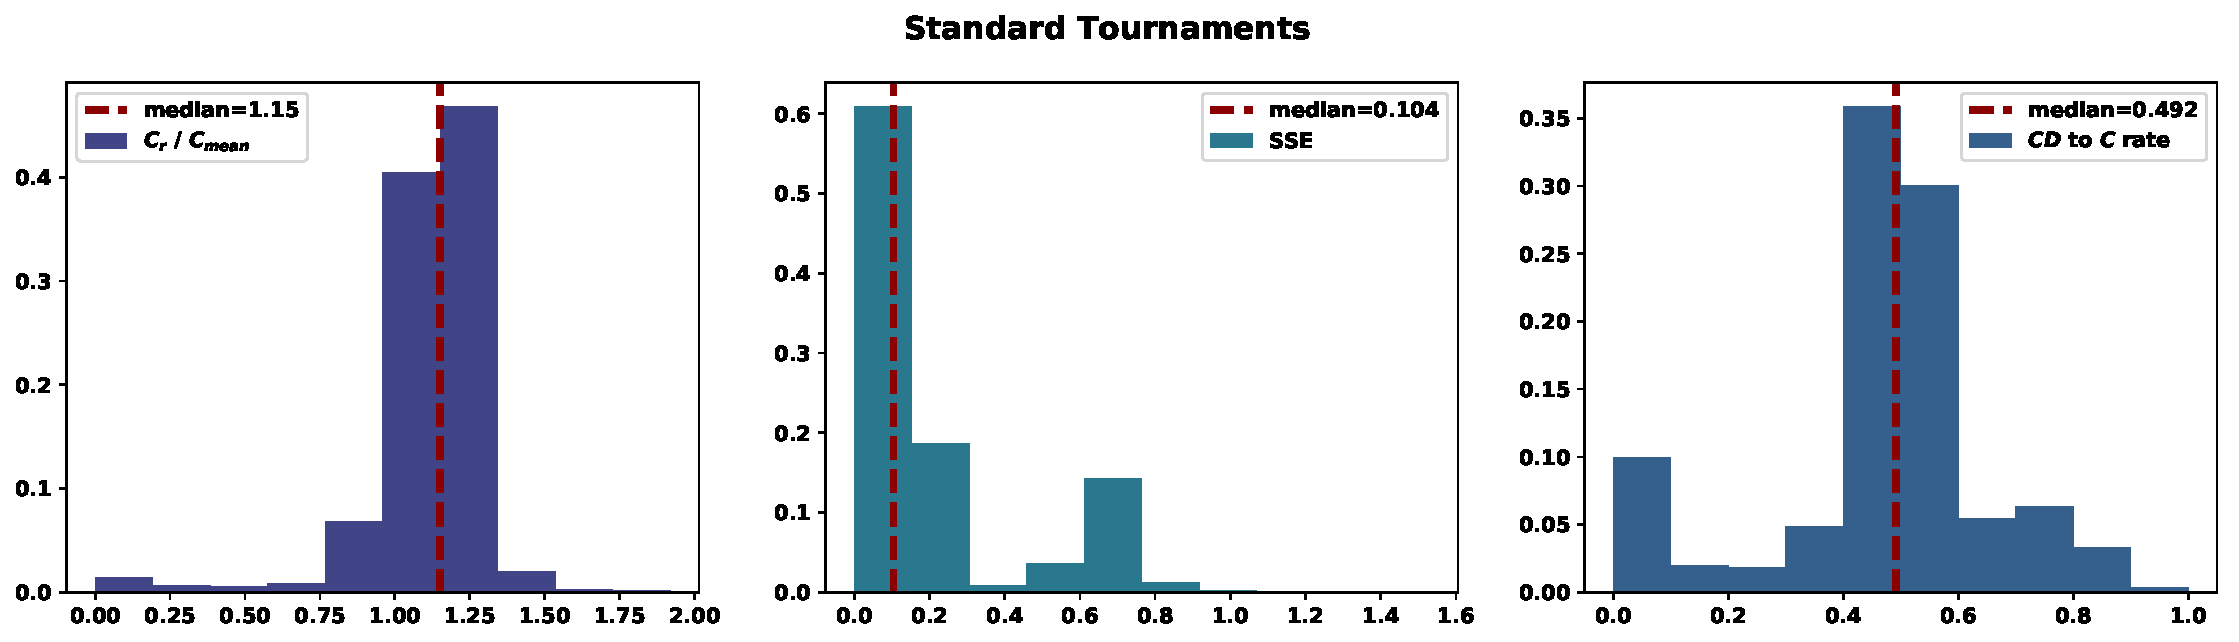
\includegraphics[width=\textwidth]{../images/standard_discussion.pdf}
        \caption{Distributions of \(C_r / C_{\text{mean}}\), SSE and \(CD\) to \(C\) ratio
        for the winners of standard tournaments. A
        value of \(C_r / C_{\text{mean}} = 1\) imply that the cooperating ratio of the
        winner was the same as the mean cooperating ratio of the tournament. An SSE distribution
        skewed towards 0 indicates a extortionate behaviour by the strategy.}
        \label{fig:discussion_standard}
\end{figure}

Similarly for the rest of the different tournaments types, and the entire data
set the distributions of \(C_r / C_{\text{mean}}\), SSE and \(CD\) to \(C\) ratio
are given by Figures~\ref{fig:discussion_noisy},~\ref{fig:discussion_probend},
\ref{fig:discussion_probend_noisy} and~\ref{fig:discussion_entire_data}.

Based on the \(C_r / C_{\text{mean}}\) distributions the successful strategies
have adapted differently to the mean cooperator depending on the tournament
type. In noisy tournaments where the median of the distribution is at 0.67, and
thereupon the winners cooperated 67\% of the time the mean cooperator did. In
tournaments with noise and a probabilistic ending the winners cooperated 60\%,
whereas in settings that the type of the tournament can vary between all the
types the winners cooperated 67\% of the time the mean cooperator did. Lastly,
in probabilistic ending tournaments above more defecting
strategies prevail (Section~\ref{section:top_performances}), and this result is
reflected here.

\begin{figure}[!htbp]
    \centering
        \centering
        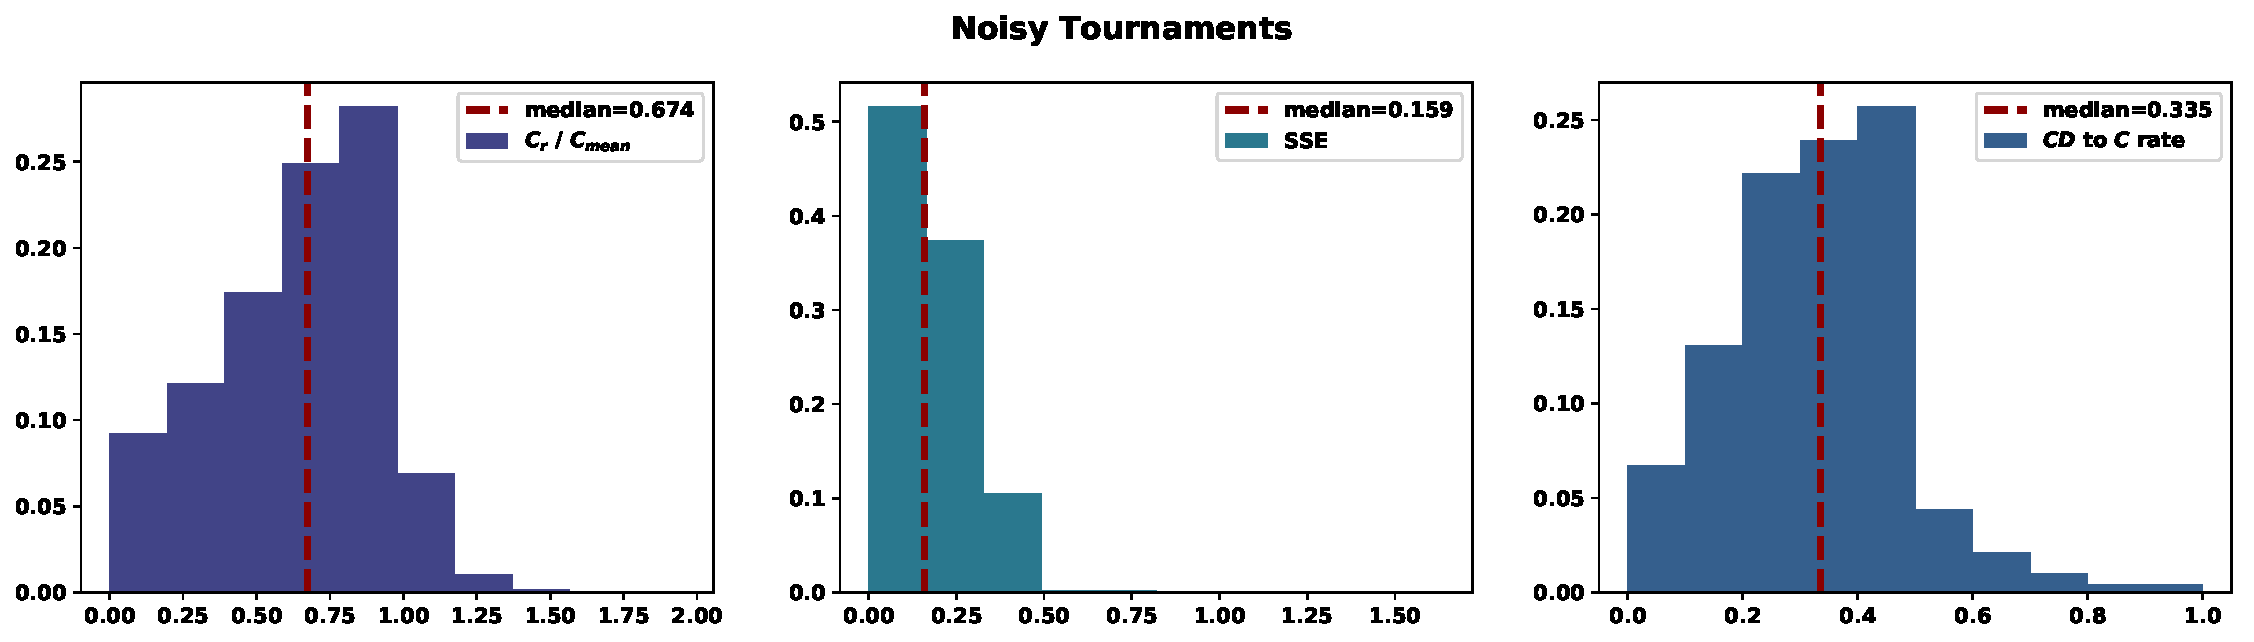
\includegraphics[width=\textwidth]{../images/noisy_discussion.pdf}
        \caption{Distributions of \(C_r / C_{\text{mean}}\), SSE and \(CD\) to \(C\) ratio
        for the winners of noisy tournaments.}
        \label{fig:discussion_noisy}
\end{figure}

The probability of noise has been observed to substantially affect optimal
behaviour.
Figure~\ref{fig:compared_to_mean_over_noise_probability} gives the ratio \(C_r /
C_{\text{mean}}\) for the winners in tournaments with noise, over the
probability of noise. From Figure~\ref{fig:noisy_discussion_over_noise} it is
clear that the cooperating only 67\% of the time the mean cooperator did is
optimal only when \(p_n \in [0.2, 0.4)\) and \(p_n \in [0.6, 0.7]\). In
environments with \(p_n < 0.1\) the winners want to be close to the mean
cooperator, similarly to standard tournaments, and as the probability of noise
is exceeding 0.5 (where the game is effectively inverted) strategies should
aim to be less and less cooperative.

Figure~\ref{fig:compared_to_mean_over_noise_probability} gives \(C_r /
C_{\text{mean}}\) for the winners over \(p_n\) in tournaments with noise and a
probabilistic ending. The optimal proportions of cooperations are different
now that the number of turns is not fixed, successful strategies
want to be more defecting that the mean cooperator, that only changes when
\(p_n\) approaches 0.5. Figure~\ref{fig:compared_to_mean_over_noise_probability}
demonstrates how the adjustments to \(C_r /C_{\text{mean}}\) change over the
noise in the to the environment, and thus supports how important adapting to
the environment is for a strategy to be successful.

\begin{figure}[!htbp]
    \centering
    \begin{subfigure}{0.485\textwidth}
        \centering
        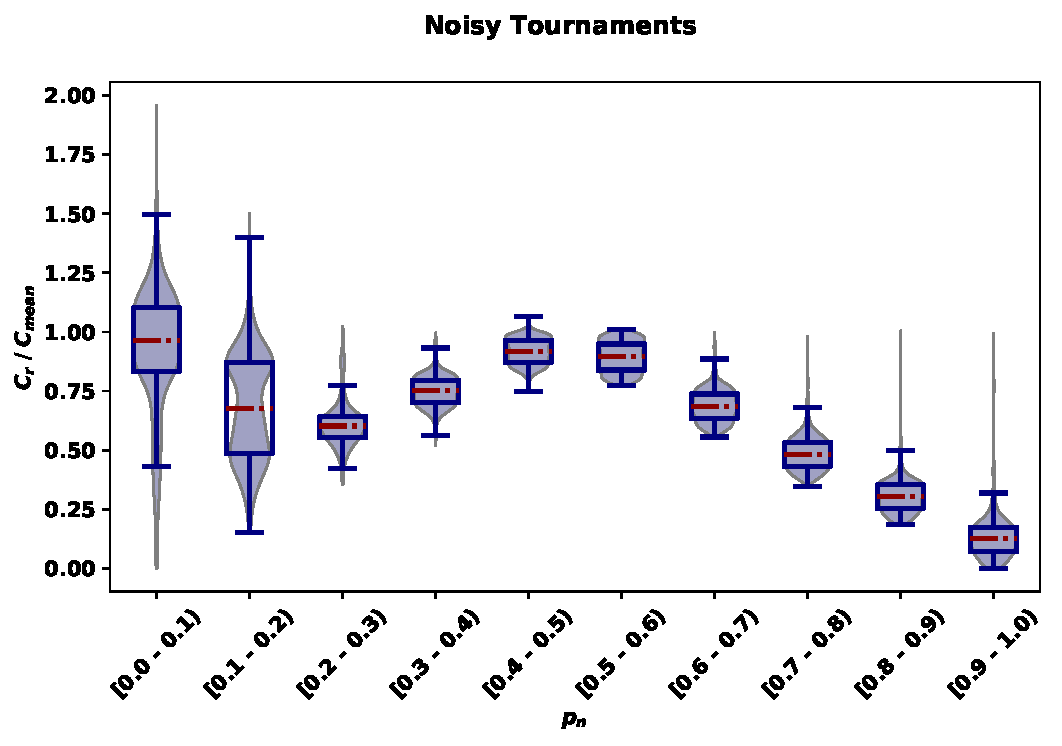
\includegraphics[width=\textwidth]{../images/noisy_discussion_over_noise.pdf}
        \caption{\(C_r / C_{\text{mean}}\) distribution for winners in noisy tournaments over
        \(p_n\).}\label{fig:noisy_discussion_over_noise}
    \end{subfigure}
    \hfill
    \begin{subfigure}{0.485\textwidth}
        \centering
        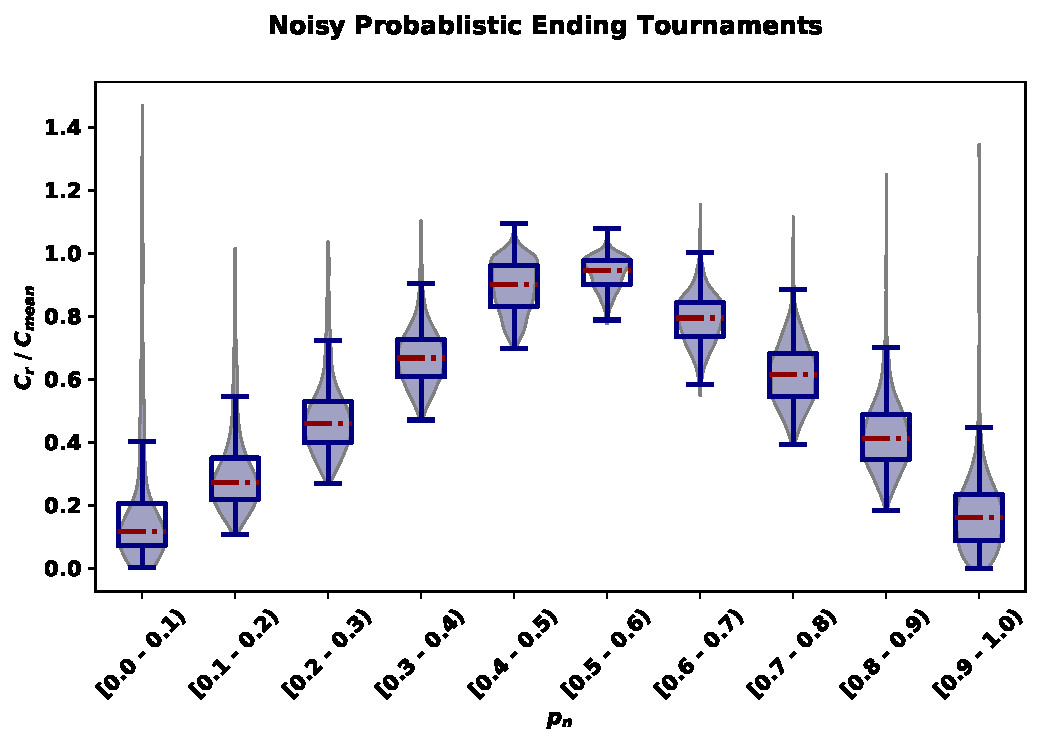
\includegraphics[width=\textwidth]{../images/noisy_probend_discussion_over_noise.pdf}
        \caption{\(C_r / C_{\text{mean}}\) distribution for winners in noisy probabilistic ending tournaments over
        \(p_n\).}\label{fig:noisy_probend_discussion_over_noise}
    \end{subfigure}
    \caption{\(C_r / C_{\text{mean}}\) distributions over intervals of \(p_n\).
    These distributions model the optimal proportion of cooperation
    compared to \(C_{\text{mean}}\) as a function of (\(p_n\)).}
    \label{fig:compared_to_mean_over_noise_probability}
\end{figure}

The distributions of the SSE across the tournament types suggest that successful
strategies exhibit some extortionate behaviour, but not constantly.
ZDs are a set of strategies that are often envious as they try to exploit their
opponents. The winners of the tournaments considered in this work are
envious, but not as much as many ZDs.
Though the exact interactions between the matches have not been recorded here,
the work of~\cite{Harper2017} which introduced the trained strategies that
appeared in the top ranked strategies of Section~\ref{section:top_performances}
did. In~\cite{Harper2017} it was shown that clever strategies managed to achieve
mutual cooperation with stronger strategies whilst exploiting the weaker
strategies. This could potentially be what is happening with the clever winners
of our analysis, and would explain the SSE distributions. This could also
be the reason why ZDs fail to appear in the tops ranks -- they try to exploit
all opponents and cannot actively adapt back to mutual cooperation against
stronger strategies, which requires more depth of memory. \footnote{Note that
ZDs also tend to perform poorly in population games for a similar reason: they
attempt to exploit other players using ZDs, failing to form a cooperative
subpopulation. This makes them good invaders but poor resisters of invasion.}

\begin{figure}[!htbp]
    \centering
        \centering
        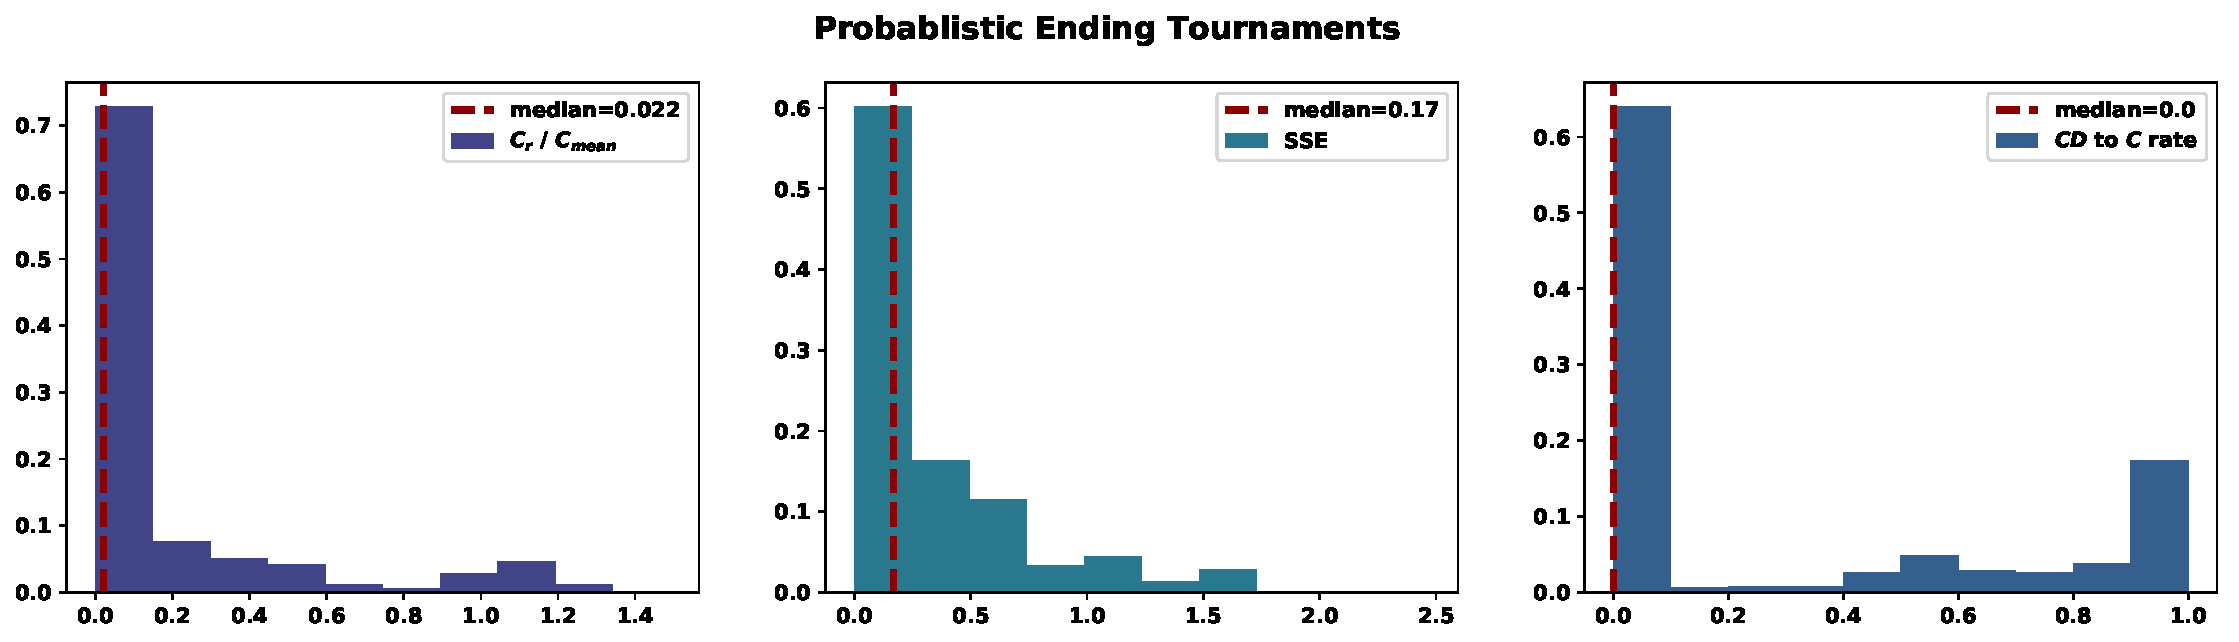
\includegraphics[width=\textwidth]{../images/probend_discussion.pdf}
        \caption{Distributions of \(C_r / C_{\text{mean}}\), SSE and \(CD\) to \(C\) ratio
        for the winners of probabilistic ending tournaments.}
        \label{fig:discussion_probend}
\end{figure}

The distributions of the \(CD\) to \(C\) rate evaluate the behaviour of a
successful strategy after its opponent has defected against it. In standard
tournaments it was observed that a successful strategy reciprocates with a
probability of 0.5, and in a setting that the type
of the tournament can vary between all the examined types a winning strategy
would reciprocate on average with a probability of 0.58. In
tournaments with noise a strategy is less likely to cooperate following a
defection compared to standard tournaments, and in probabilistic ending
tournaments a strategy will reciprocate a defection.
This leads to revisiting the recommendation of being provocable to defections made
by R. Axerlod. In fact only in tournaments with short matches should a strategy
be provocable, in the rest of the settings a strategy should be more
generous.

\begin{figure}[!htbp]
    \centering
        \centering
        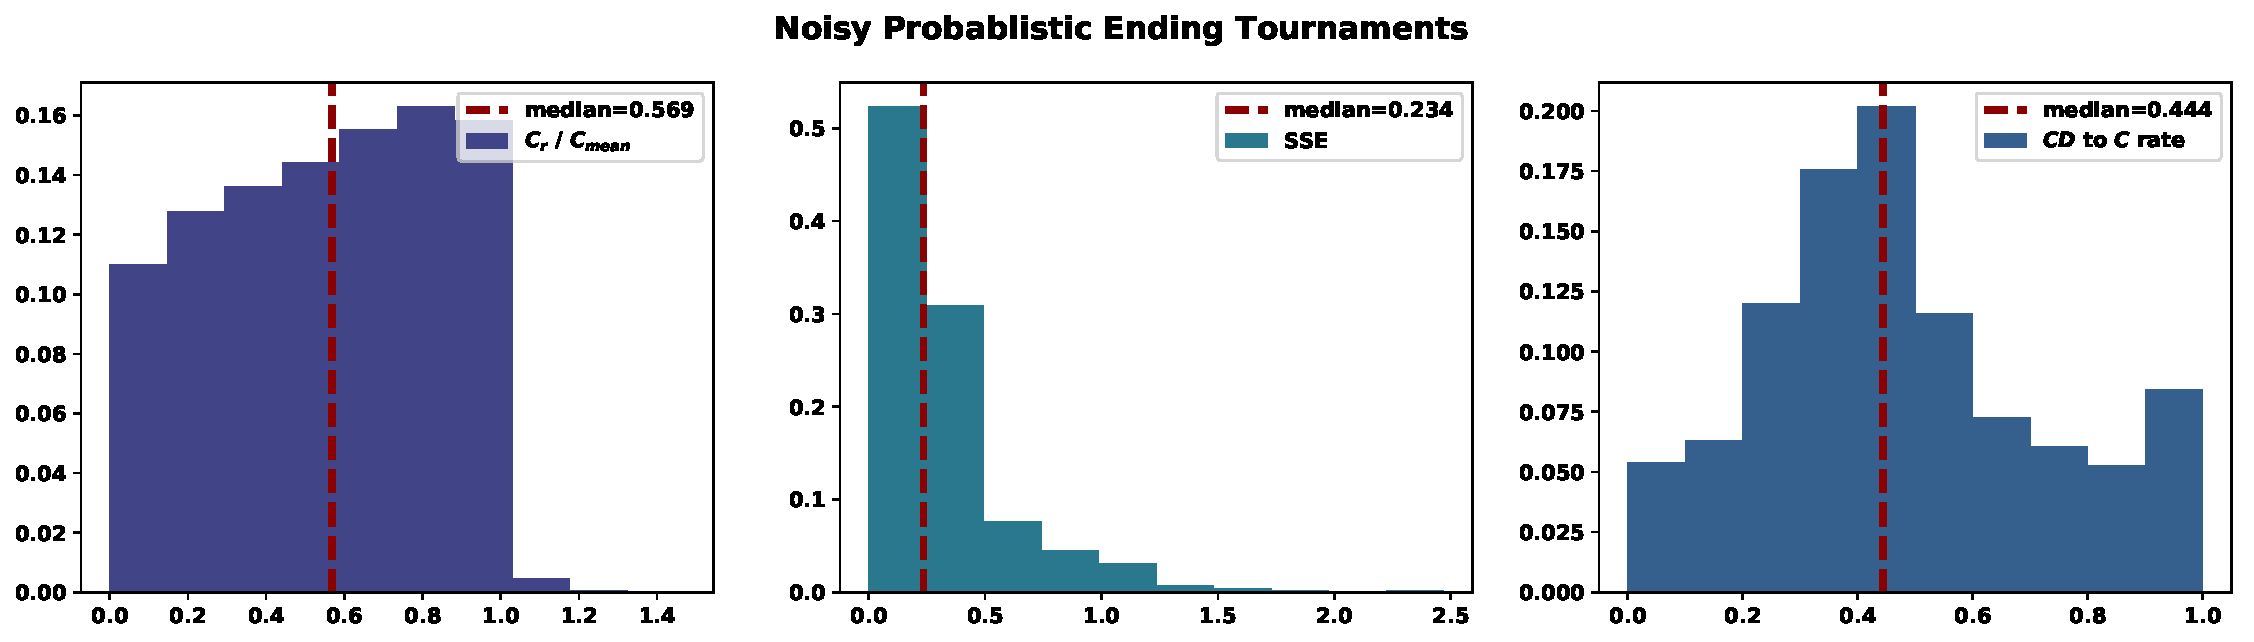
\includegraphics[width=\textwidth]{../images/probend_noisy_discussion.pdf}
        \caption{Distributions of \(C_r / C_{\text{mean}}\), SSE and \(CD\) to \(C\) ratio
        for the winners of noisy probabilistic ending tournaments.}
        \label{fig:discussion_probend_noisy}
\end{figure}

Further statistically significant features with strong effects include \(C_r /
C_{\text{min}}\), \(C_r / C_{\text{max}}\), \(C_{\text{min}}\) and
\(C_{\text{max}}\). These add more emphasis on how important it is for a  a
strategy to adapt to its environment. Finally, the features number of turns,
repetitions and the probabilities of noise and the game ending had no
significant effects based on the multivariate regression models.

\begin{figure}[!htbp]
    \centering
        \centering
        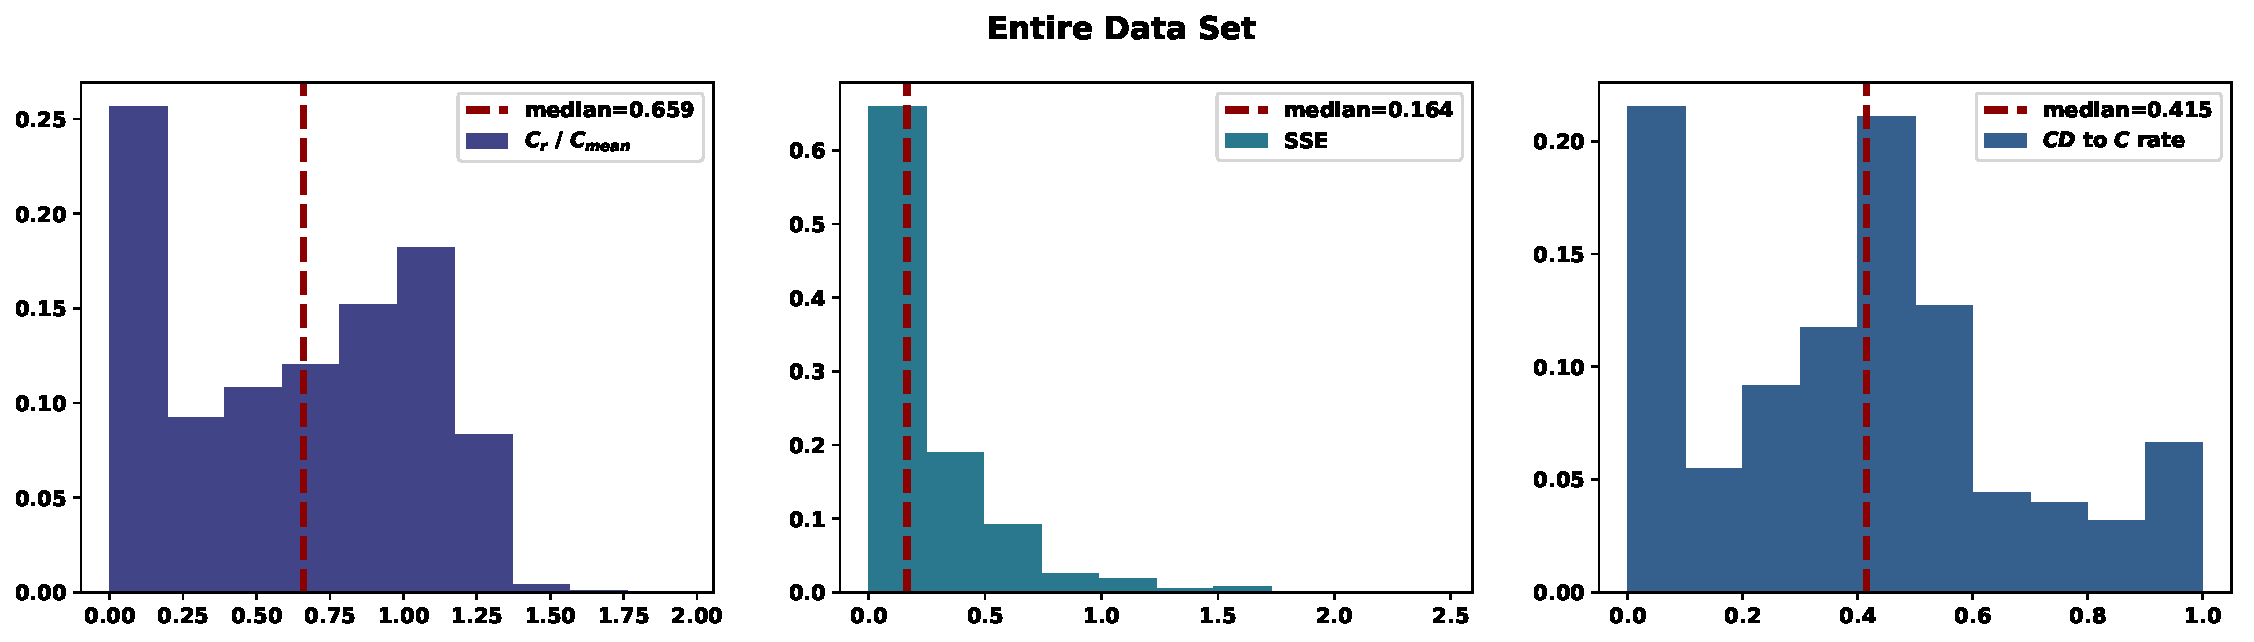
\includegraphics[width=\textwidth]{../images/entire_data_discussion.pdf}
        \caption{Distributions of \(C_r / C_{\text{mean}}\), SSE and \(CD\) to \(C\) ratio
        for the winners over the tournaments of the entire data set.}
        \label{fig:discussion_entire_data}
\end{figure}

A third method that evaluates the importance of the features in
Table~\ref{table:manual_features} using clustering and random forests can be found in
the Appendix~\ref{app:clustering}. The results uphold the outcomes of the
correlation and multivariate regression. It also evaluates the effects
of the whether or not a strategy is stochastic, makes use of the knowledge of the utility values, or makes use of match length. These were not evaluated by the methods above because there are binary variables.
The results showed that they have no significant effect on a strategy's
performance.

\section{Discussion}\label{section:conclusion}

This manuscript explored the performance of \numberofstrategies strategies of
the IPD in \numberofalltournaments computer tournaments. The collection of
computer tournaments presented here is the largest and most diverse collection in the
literature. The \numberofstrategies strategies are drawn from the APL and include
strategies from the IPD literature. The computer tournaments include tournaments of
four different types.

So what is the best way of playing the IPD? And is
there a single dominant strategy for the IPD? 

There was not a single strategy
within the collection of the \numberofstrategies strategies that managed to
perform well in all the tournaments variations it competed in. Even if on
average a strategy ranked highly in a specific environment this did not
guarantee its success over the different tournament types. Nevertheless, in
Sections~\ref{section:top_performances}
and~\ref{section:evaluation_of_performance} we examined the best performing
strategies across various tournament types and analysed their salient features.
this demonstrated that there are properties associated with the success of
strategies which in fact contradict the originally suggested properties of R.
Axelrod~\cite{Axelrod1981}.

We showed that complex or \textbf{clever} strategies can be effective, whether
trained against a corpus of possible opponents or purposely designed to mitigate
the impact of noise such as the DBS strategy. Moreover, we found some
strategies designed or trained for noisy environments were also highly ranked in
noise-free tournaments which reinforces the idea that strategies'
complexity/cleverness is not necessarily a liability, rather it can confer
adaptability to a more diverse set of environments.
We also showed that while the type of exploitation attempted by ZDs is
not typically effective in standard tournaments, \textbf{envious} strategies
capable of both exploiting and not their opponents can be highly successful.
Based on the results of~\cite{Harper2017} this could be because they are
selectively exploiting weaker opponents while mutually cooperating with stronger
opponents. Highly noisy or tournaments with short matches also favoured envious
strategies. These environments mitigated the value of being nice. Uncertainty
enables exploitation, reducing the ability of maintaining or enforcing mutual
cooperation, while triggering grudging strategies to switch from typically
cooperating to typically defecting.

The features analysis of the best performing strategies demonstrated that a
strategy should reciprocate, as suggested by R. Axelrod, but it should relax its
readiness to do so and be more \textbf{generous}. For noisy environments this is
inline with the results of~\cite{Bendor1991, Donninger1986, Molander1985,
Hammerstein1984}, however, we also showed that generosity pays off even in
standard settings, and that in fact the only setting a strategy would want to be
too provocable is when the matches are not long. Forgiveness as defined by R.
Axerlod was not explored here. This was mainly because the two round states were
not recorded during the data collection. That is something we would aim to
incorporate in future work.
The features analysis also concluded that
there is a significant importance in \textbf{adapting to the environment}, and
more specifically, to the mean cooperator. 
In standard tournaments a strategy would aim to be the
mean the cooperator while in noisy tournaments the best performing players
cooperate at a lower rate than the tournament population on average.
Moreover, the manner in which a
strategy achieves a given cooperation rate relative to the tournament population
average is important.

This could potentially explain the early success of TFT. TFT naturally achieves
a cooperation rate near $C_{\text{mean}}$ by virtue of copying its opponent's
last move while also minimizing instances where it is exploited by an opponent
(cooperating while the opponent defects), at least in non-noisy tournaments. It
could also explain why Tit For \(N\) Tats does not fare well for $N > 1$ -- it
fails to achieve the proper cooperation ratio by tolerating too many defections.

Similarly, our results could suggest an explanation regarding the intuitively
unexpected effectiveness of memory-one strategies historically. Given that among
the important features associated with success are the relative cooperation rate
to the population average and the four memory-one probabilities of cooperating
conditional on the previous round of play, these features can be optimized by a
memory-one strategy such as TFT. Usage of more history becomes valuable when
there are exploitable opponent patterns. This is indicated by the importance of
SSE as a feature, showing that the first-approximation provided by a memory-one
strategy is no longer sufficient.

These results highlight a central idea in evolutionary game theory in this
context: the fitness landscape is a function of the population (where fitness in
this case is tournament performance). While that may seem obvious now, it shows
why historical tournament results on small or arbitrary populations of
strategies have so often failed to produce generalizable results.

Overall, the five properties successful strategies need to have in a IPD competition
based on the analysis that has been presented in this manuscript are:

\begin{itemize}
    \item Be ``nice'' in non-noisy environments or when game lengths are longer
    \item Be provocable but also generous when game lengths are longer
    \item Be a little bit envious
    \item Be clever
    \item Adapt to the environment (including the population of strategies).
\end{itemize}

The data set described in this work contains the largest number of IPD tournaments,
to the authors knowledge. The raw data set is available at~\cite{raw_data} and the
processed data at~\cite{data}. Further data mining
could be applied and provide new insights in the field.

\bibliographystyle{plain}
\bibliography{bibliography}

\section{Acknowledgements}

A variety of software have been used in this work:

\begin{itemize}
    \item The Axelrod-Python library for IPD simulations~\cite{axelrodproject}.
    \item The Matplotlib library for visualisation~\cite{hunter2007matplotlib}.
    \item The Numpy library for data manipulation~\cite{walt2011numpy}.
    \item The scikit-learn library for data analysis~\cite{scikit-learn}.
\end{itemize}

\appendix

\section{Parameters Summary}\label{app:parameters}

All the parameters used in this manuscript alongside their explanation are
given by Table~\ref{table:parameters_summary}.

\begin{table}[!htbp]
    \begin{center}
    \resizebox{.7\textwidth}{!}{
    \begin{tabular}{ll}
    \toprule
Feature & Explanation \\
 \midrule
SSE                       & A measure of how far a strategy is from extortionate behaviour defined in~\cite{Knight2019}. \\
$C_{\text{max}}$          & The biggest cooperating rate in the tournament. \\
$C_{\text{min}}$          & The smallest cooperating rate in the tournament. \\
$C_{\text{median}}$       & The median cooperating rate in the tournament. \\
$C_{\text{mean}}$         & The mean cooperating rate in the tournament. \\
$C_r$ / $C_{\text{max}}$    & A strategy's cooperating rate divided by the maximum cooperating rate in the tournament. \\
$C_{\text{min}}$ / $C_r$    & The minimum in the tournament divided by a strategy's cooperating rate. \\
$C_r$ / $C_{\text{median}}$ & A strategy's cooperating rate divided by the median cooperating rate in the tournament. \\
$C_r$ / $C_{\text{mean}}$   & A strategy's cooperating rate divided by the mean cooperating rate in the tournament. \\
$C_r$                       & The cooperating rate of a strategy. \\
$CC$ to $C$ rate            & The probability a strategy will cooperate after a mutual cooperation. \\
$CD$ to $C$ rate            & The probability a strategy will cooperate after being betrayed by the opponent. \\
$DC$ to $C$ rate            & The probability a strategy will cooperate after betraying the opponent. \\
$DD$ to $C$ rate            & The probability a strategy will cooperate after a mutual defection. \\
$p_n$                       & The probability of a player's action being flipped at each interaction. \\
$n$                         & The number of turns in a match. \\
$p_e$                       & The probability of a match ending in the next turn. \\
$N$                         & The number of strategies in the tournament. \\
$k$                         & The number that a given tournament is repeated. \\
    \bottomrule
        \end{tabular}}
    \end{center}
    \caption{The features which are included in the performance evaluation analysis.}\label{table:parameters_summary}
\end{table}

\section{Correlation coefficients}\label{app:correlations}

A graphical representation of the correlation coefficients for the features in
Table~\ref{table:manual_features}.

\begin{figure}[!htbp]
        \begin{center}
            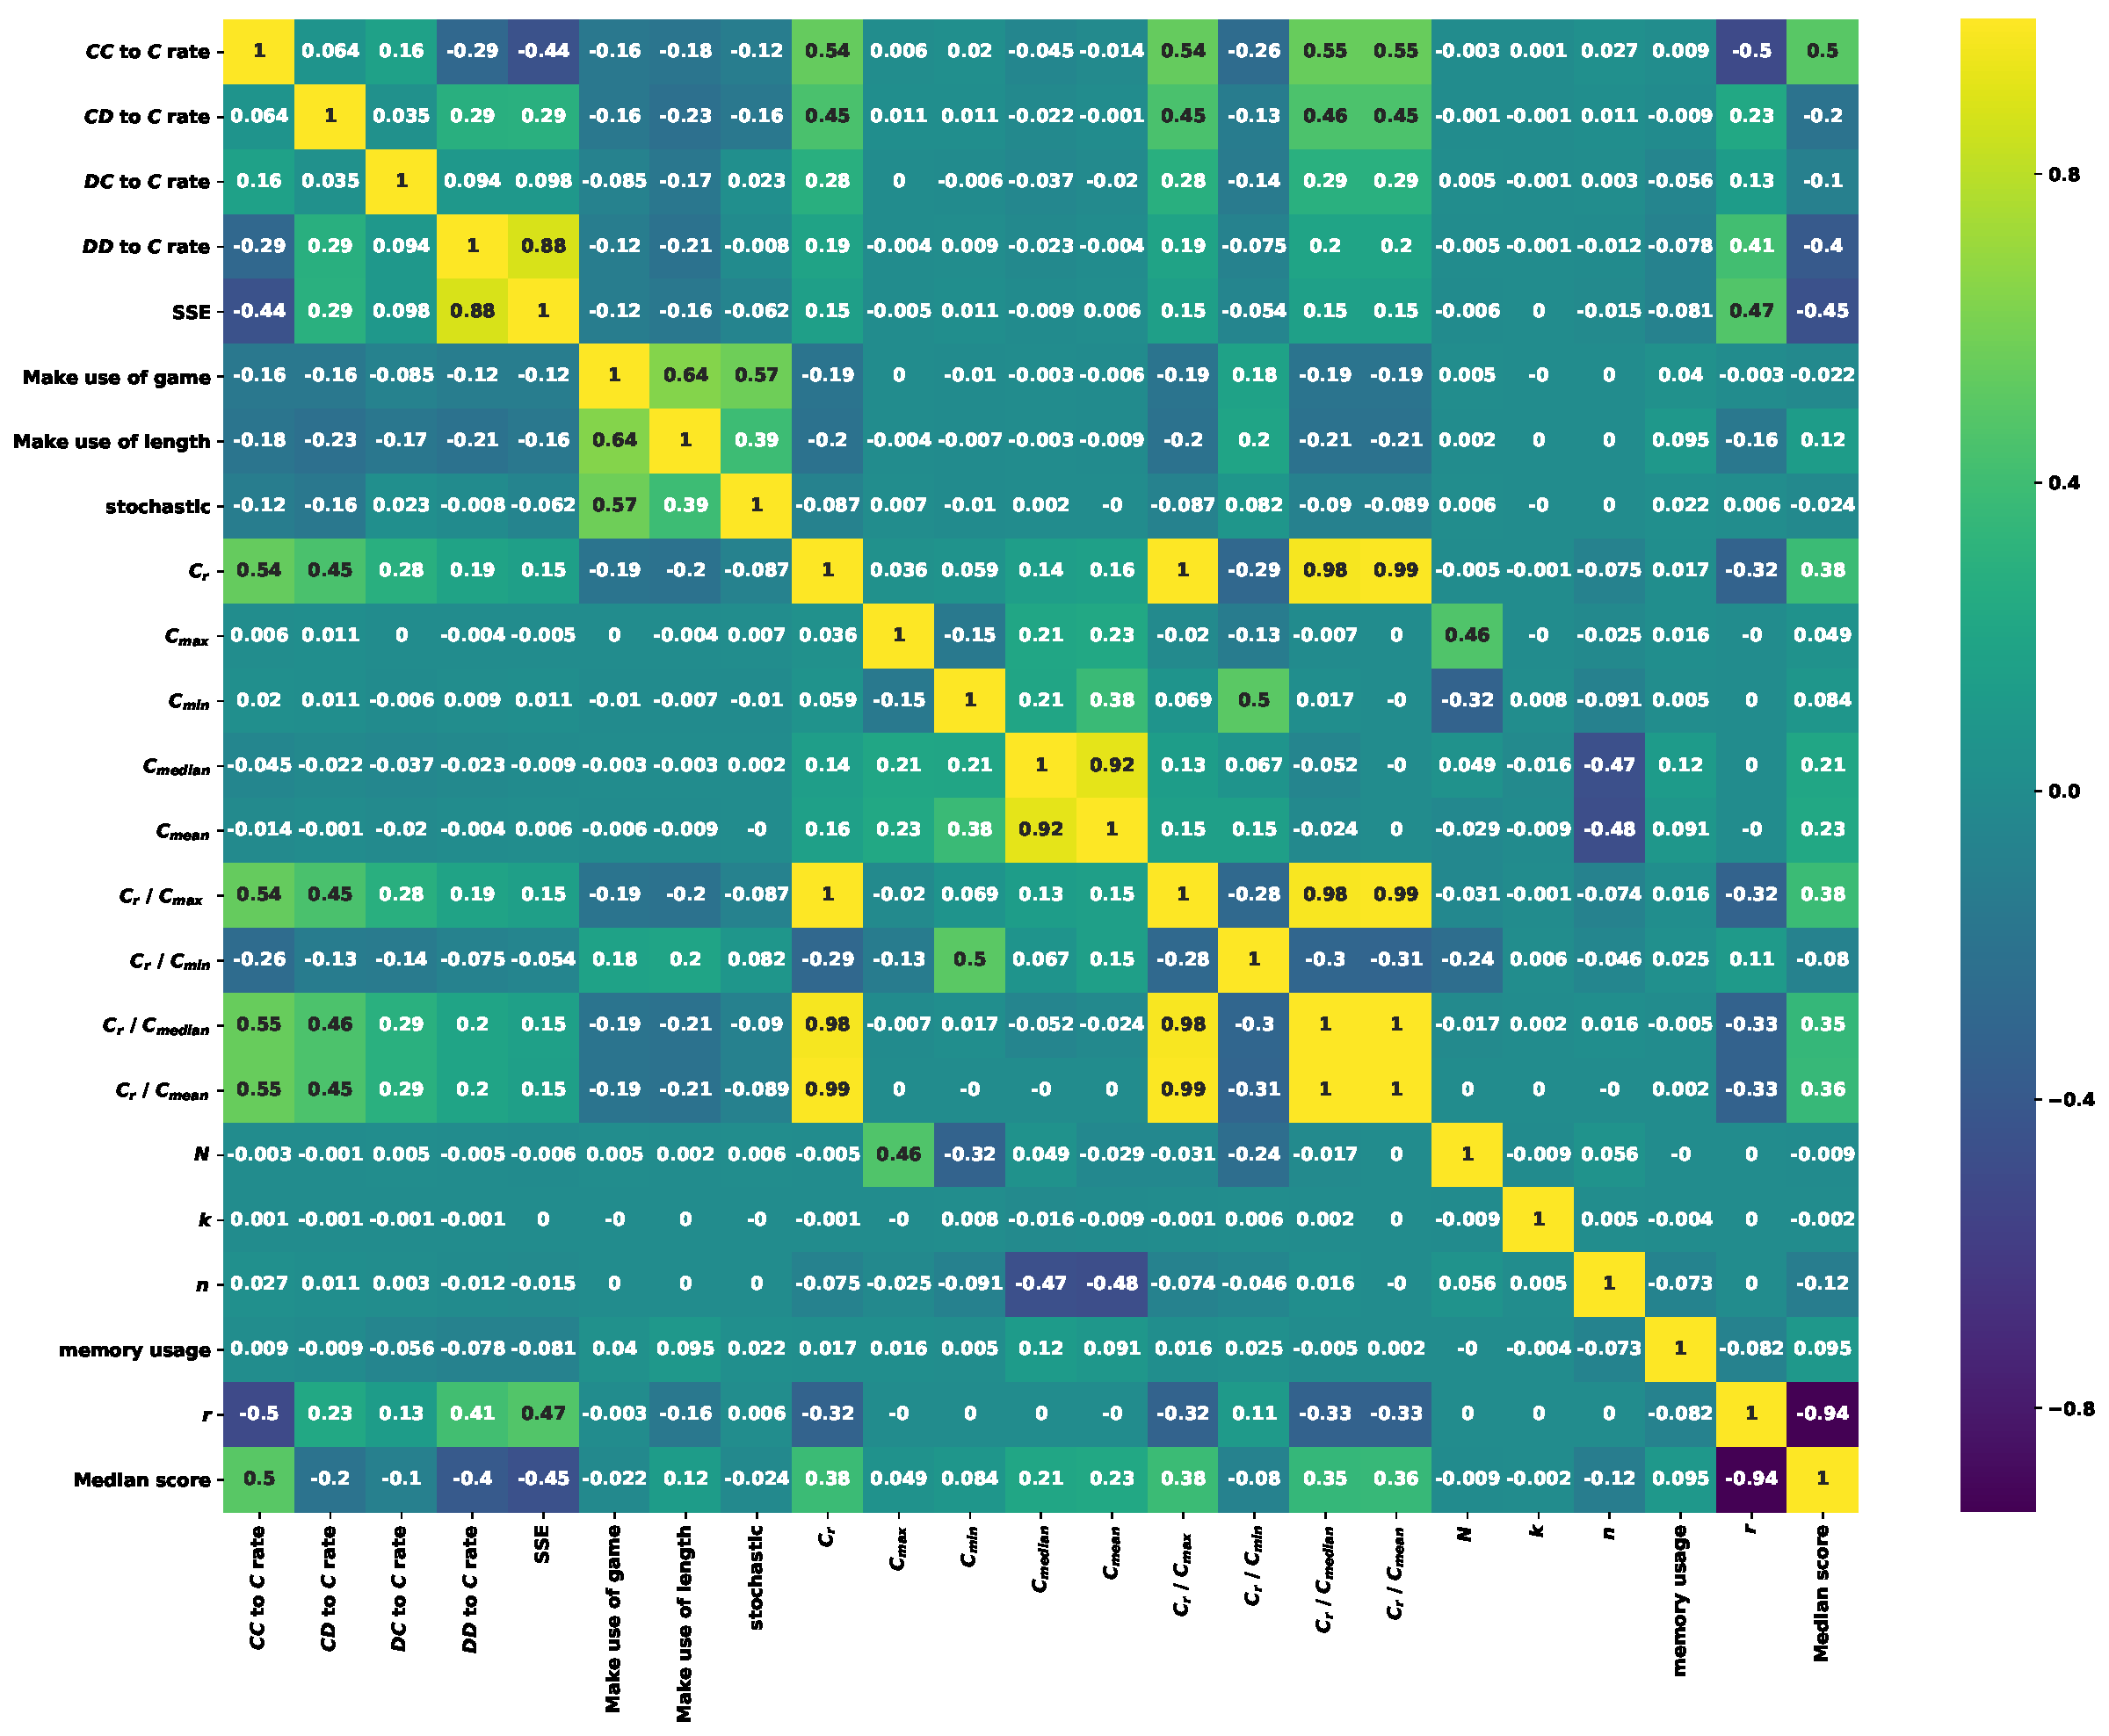
\includegraphics[width=.75\linewidth]{../images/standard_correlation_plot.pdf}
        \end{center}
        \caption{Correlation coefficients of features in Table~\ref{table:manual_features}
        for standard tournaments}
\end{figure}
\begin{figure}[!htbp]
    \begin{center}
        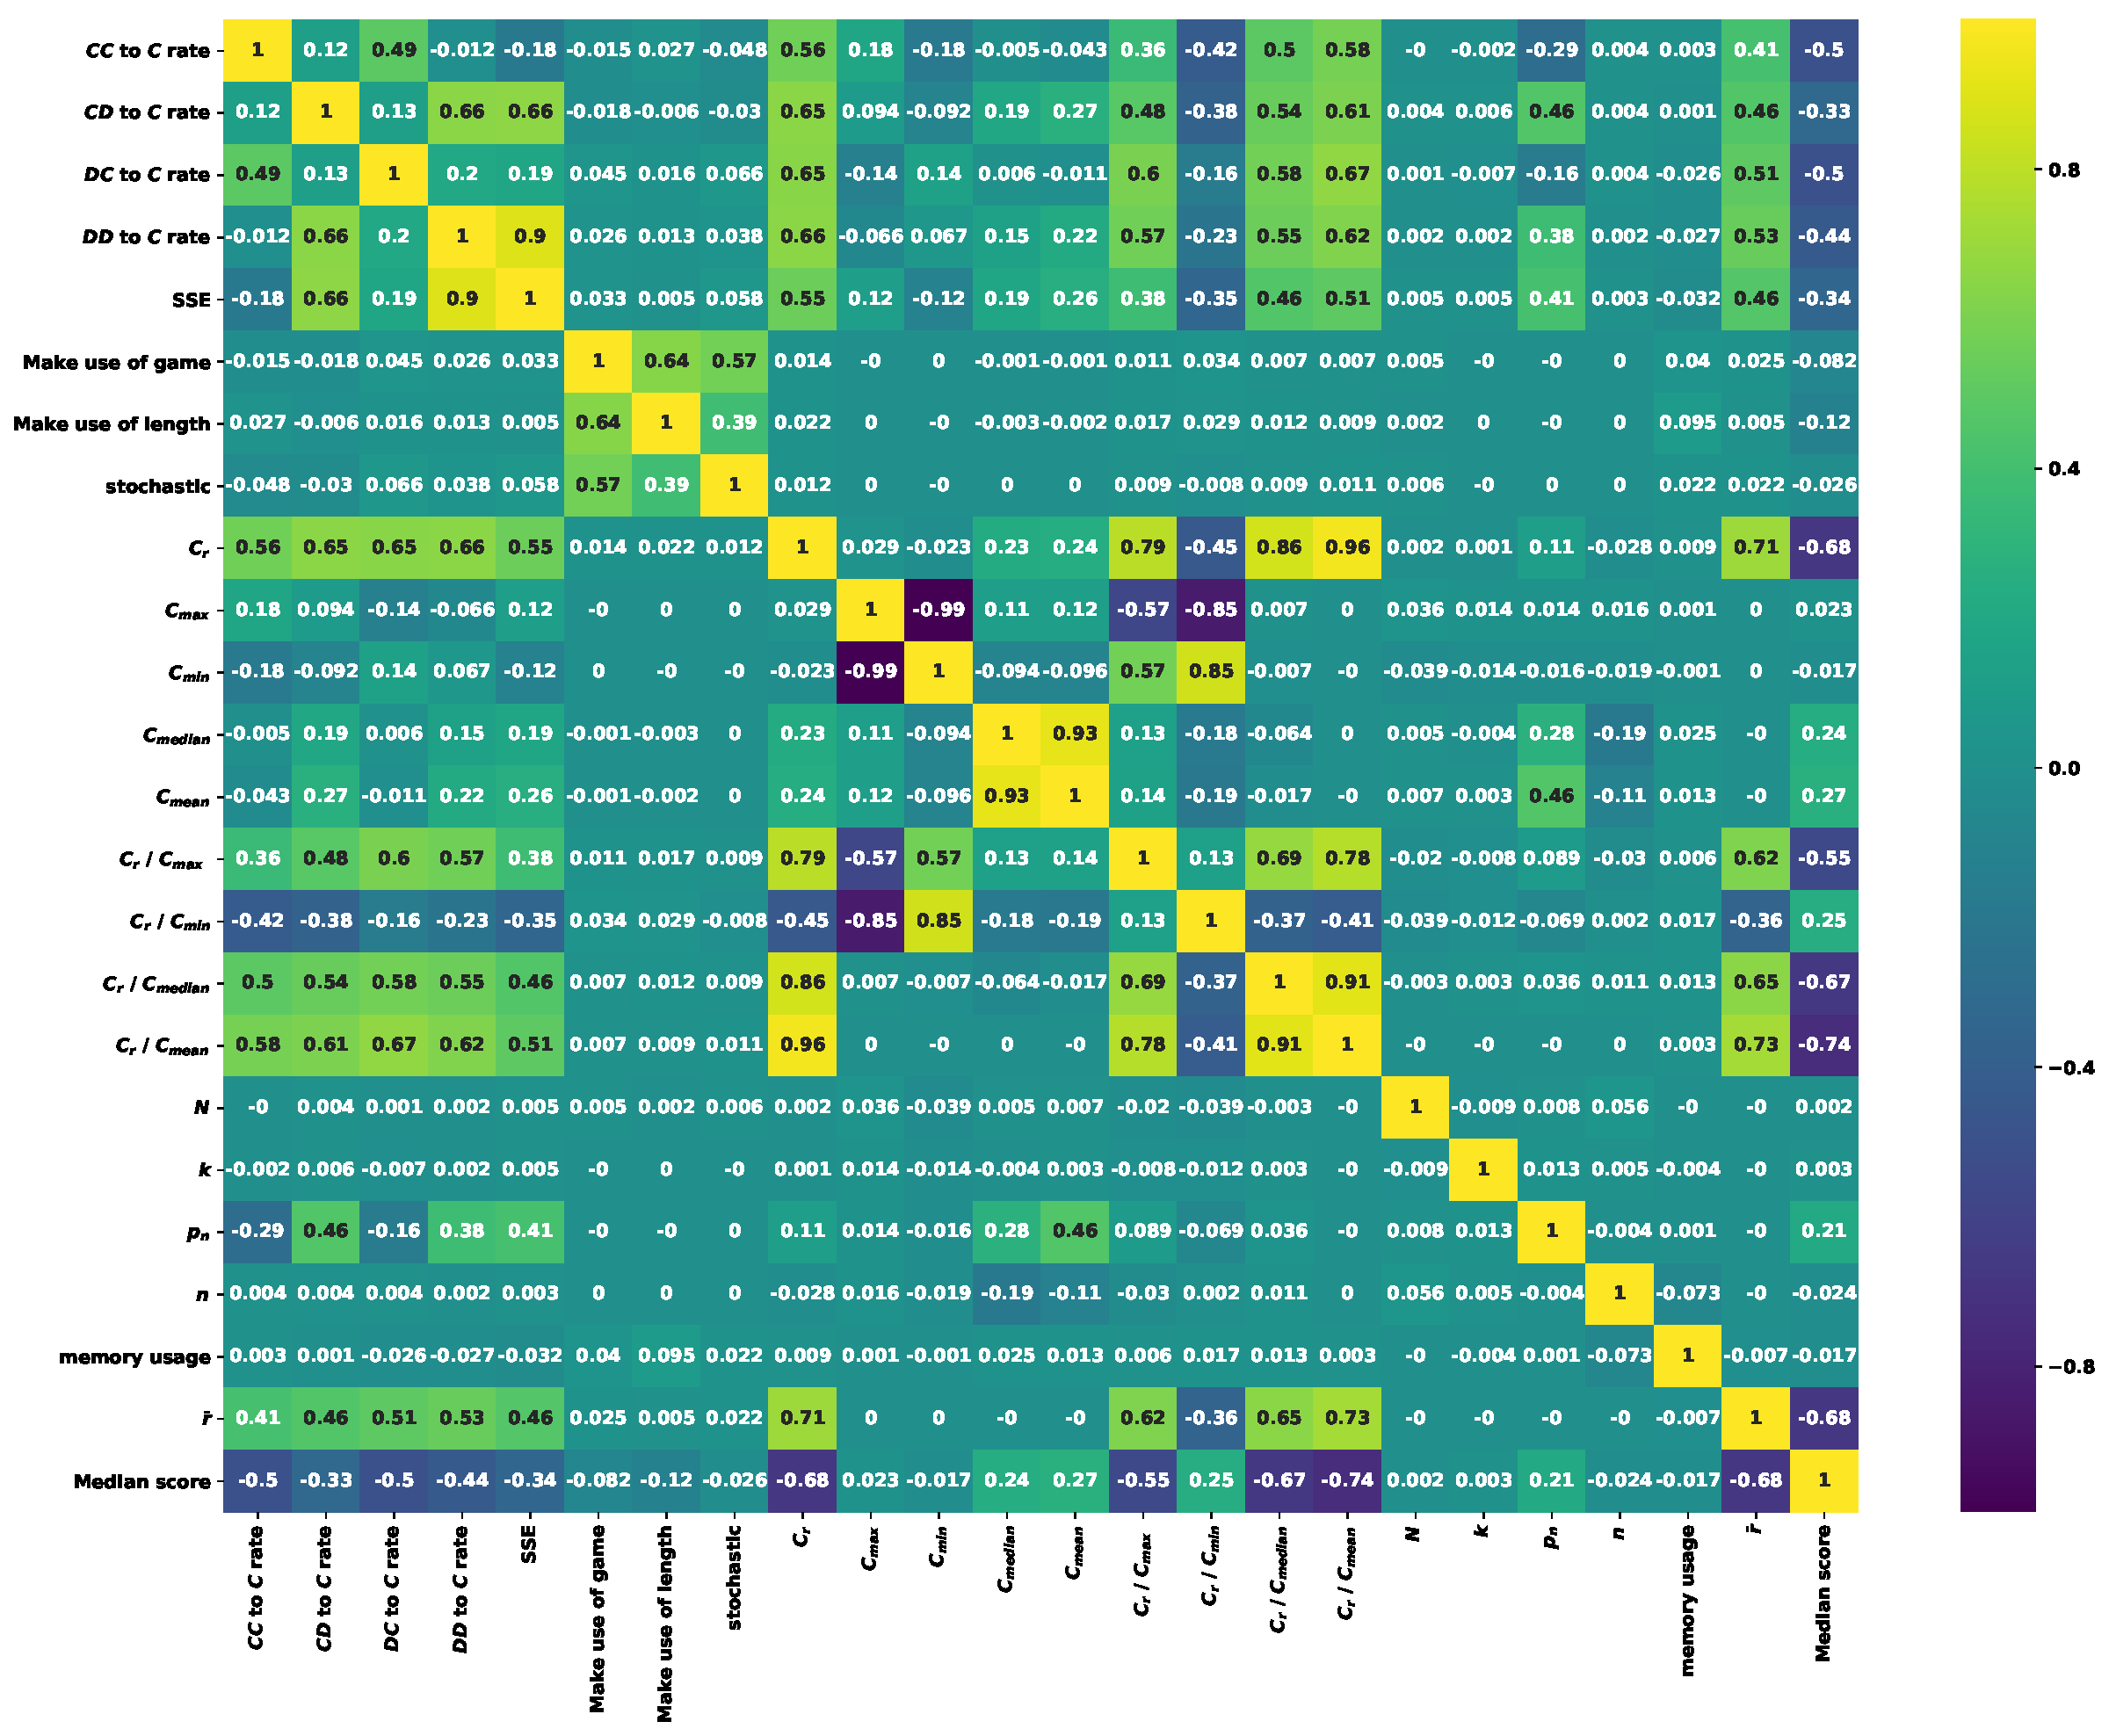
\includegraphics[width=.75\linewidth]{../images/noise_correlation_plot.pdf}
    \end{center}
    \caption{Correlation coefficients of features in Table~\ref{table:manual_features}
    for noisy tournaments}
\end{figure}
\begin{figure}[!htbp]
    \begin{center}
        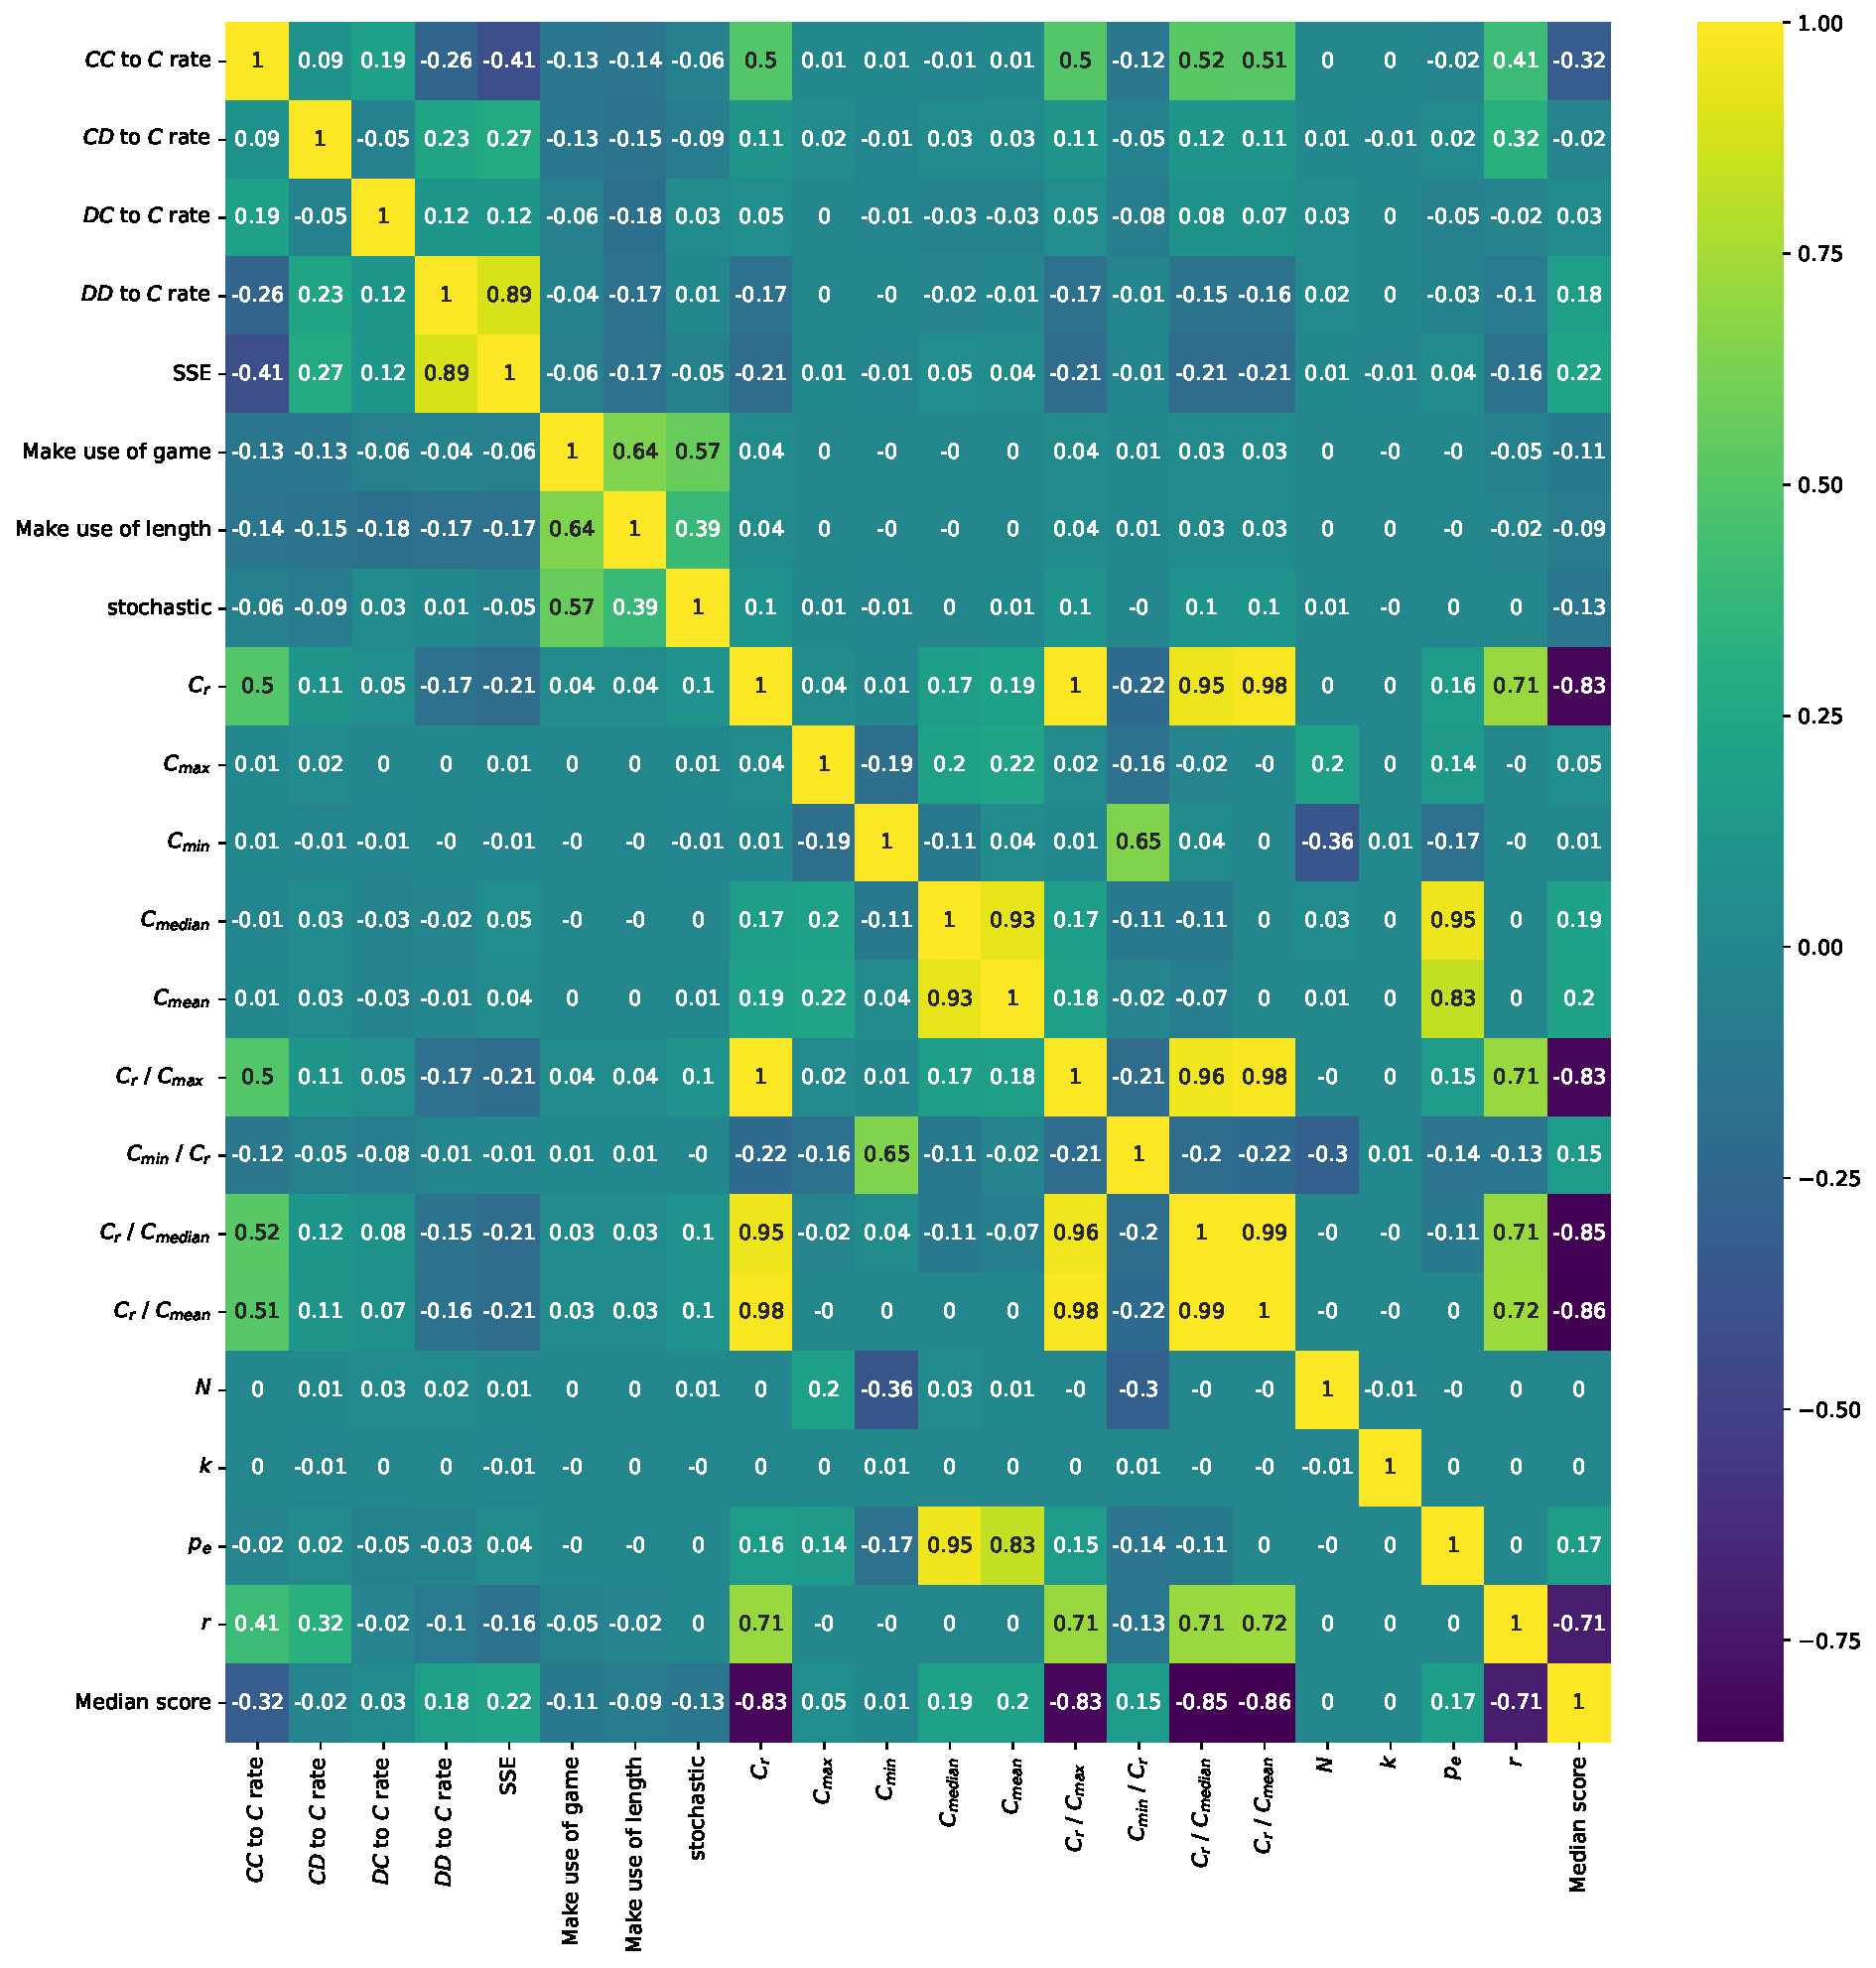
\includegraphics[width=.75\linewidth]{../images/probend_correlation_plot.pdf}
    \end{center}
    \caption{Correlation coefficients of features in Table~\ref{table:manual_features}
    for probabilistic ending tournaments}
\end{figure}
\begin{figure}[!htbp]
    \begin{center}
        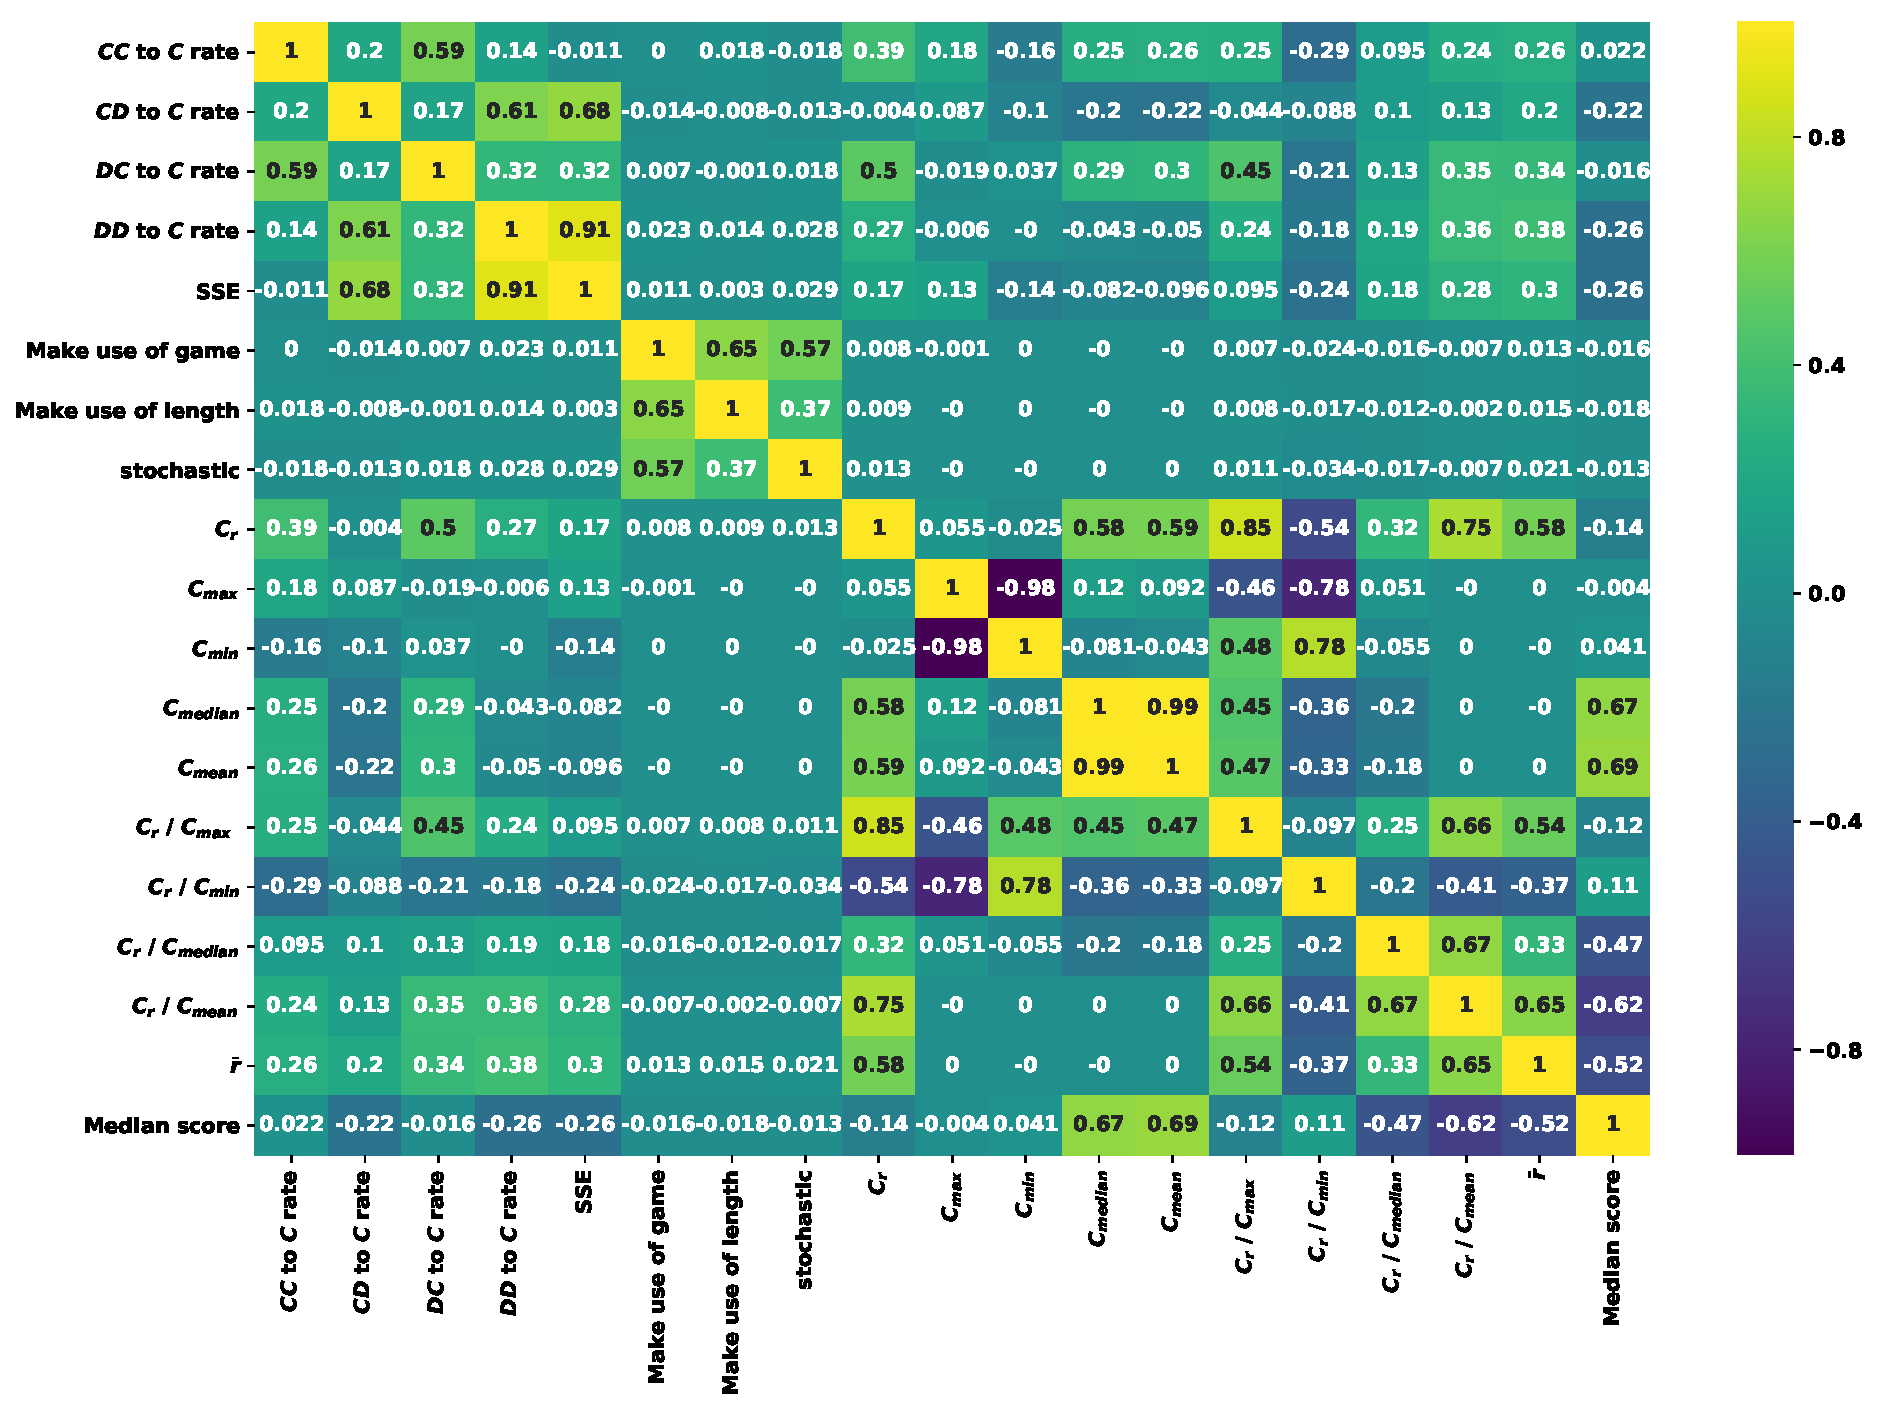
\includegraphics[width=.75\linewidth]{../images/probend_noise_correlation_plot.pdf}
    \end{center}
    \caption{Correlation coefficients of features in Table~\ref{table:manual_features}
    for noisy probabilistic ending tournaments}
\end{figure}
\begin{figure}[!htbp]
    \begin{center}
        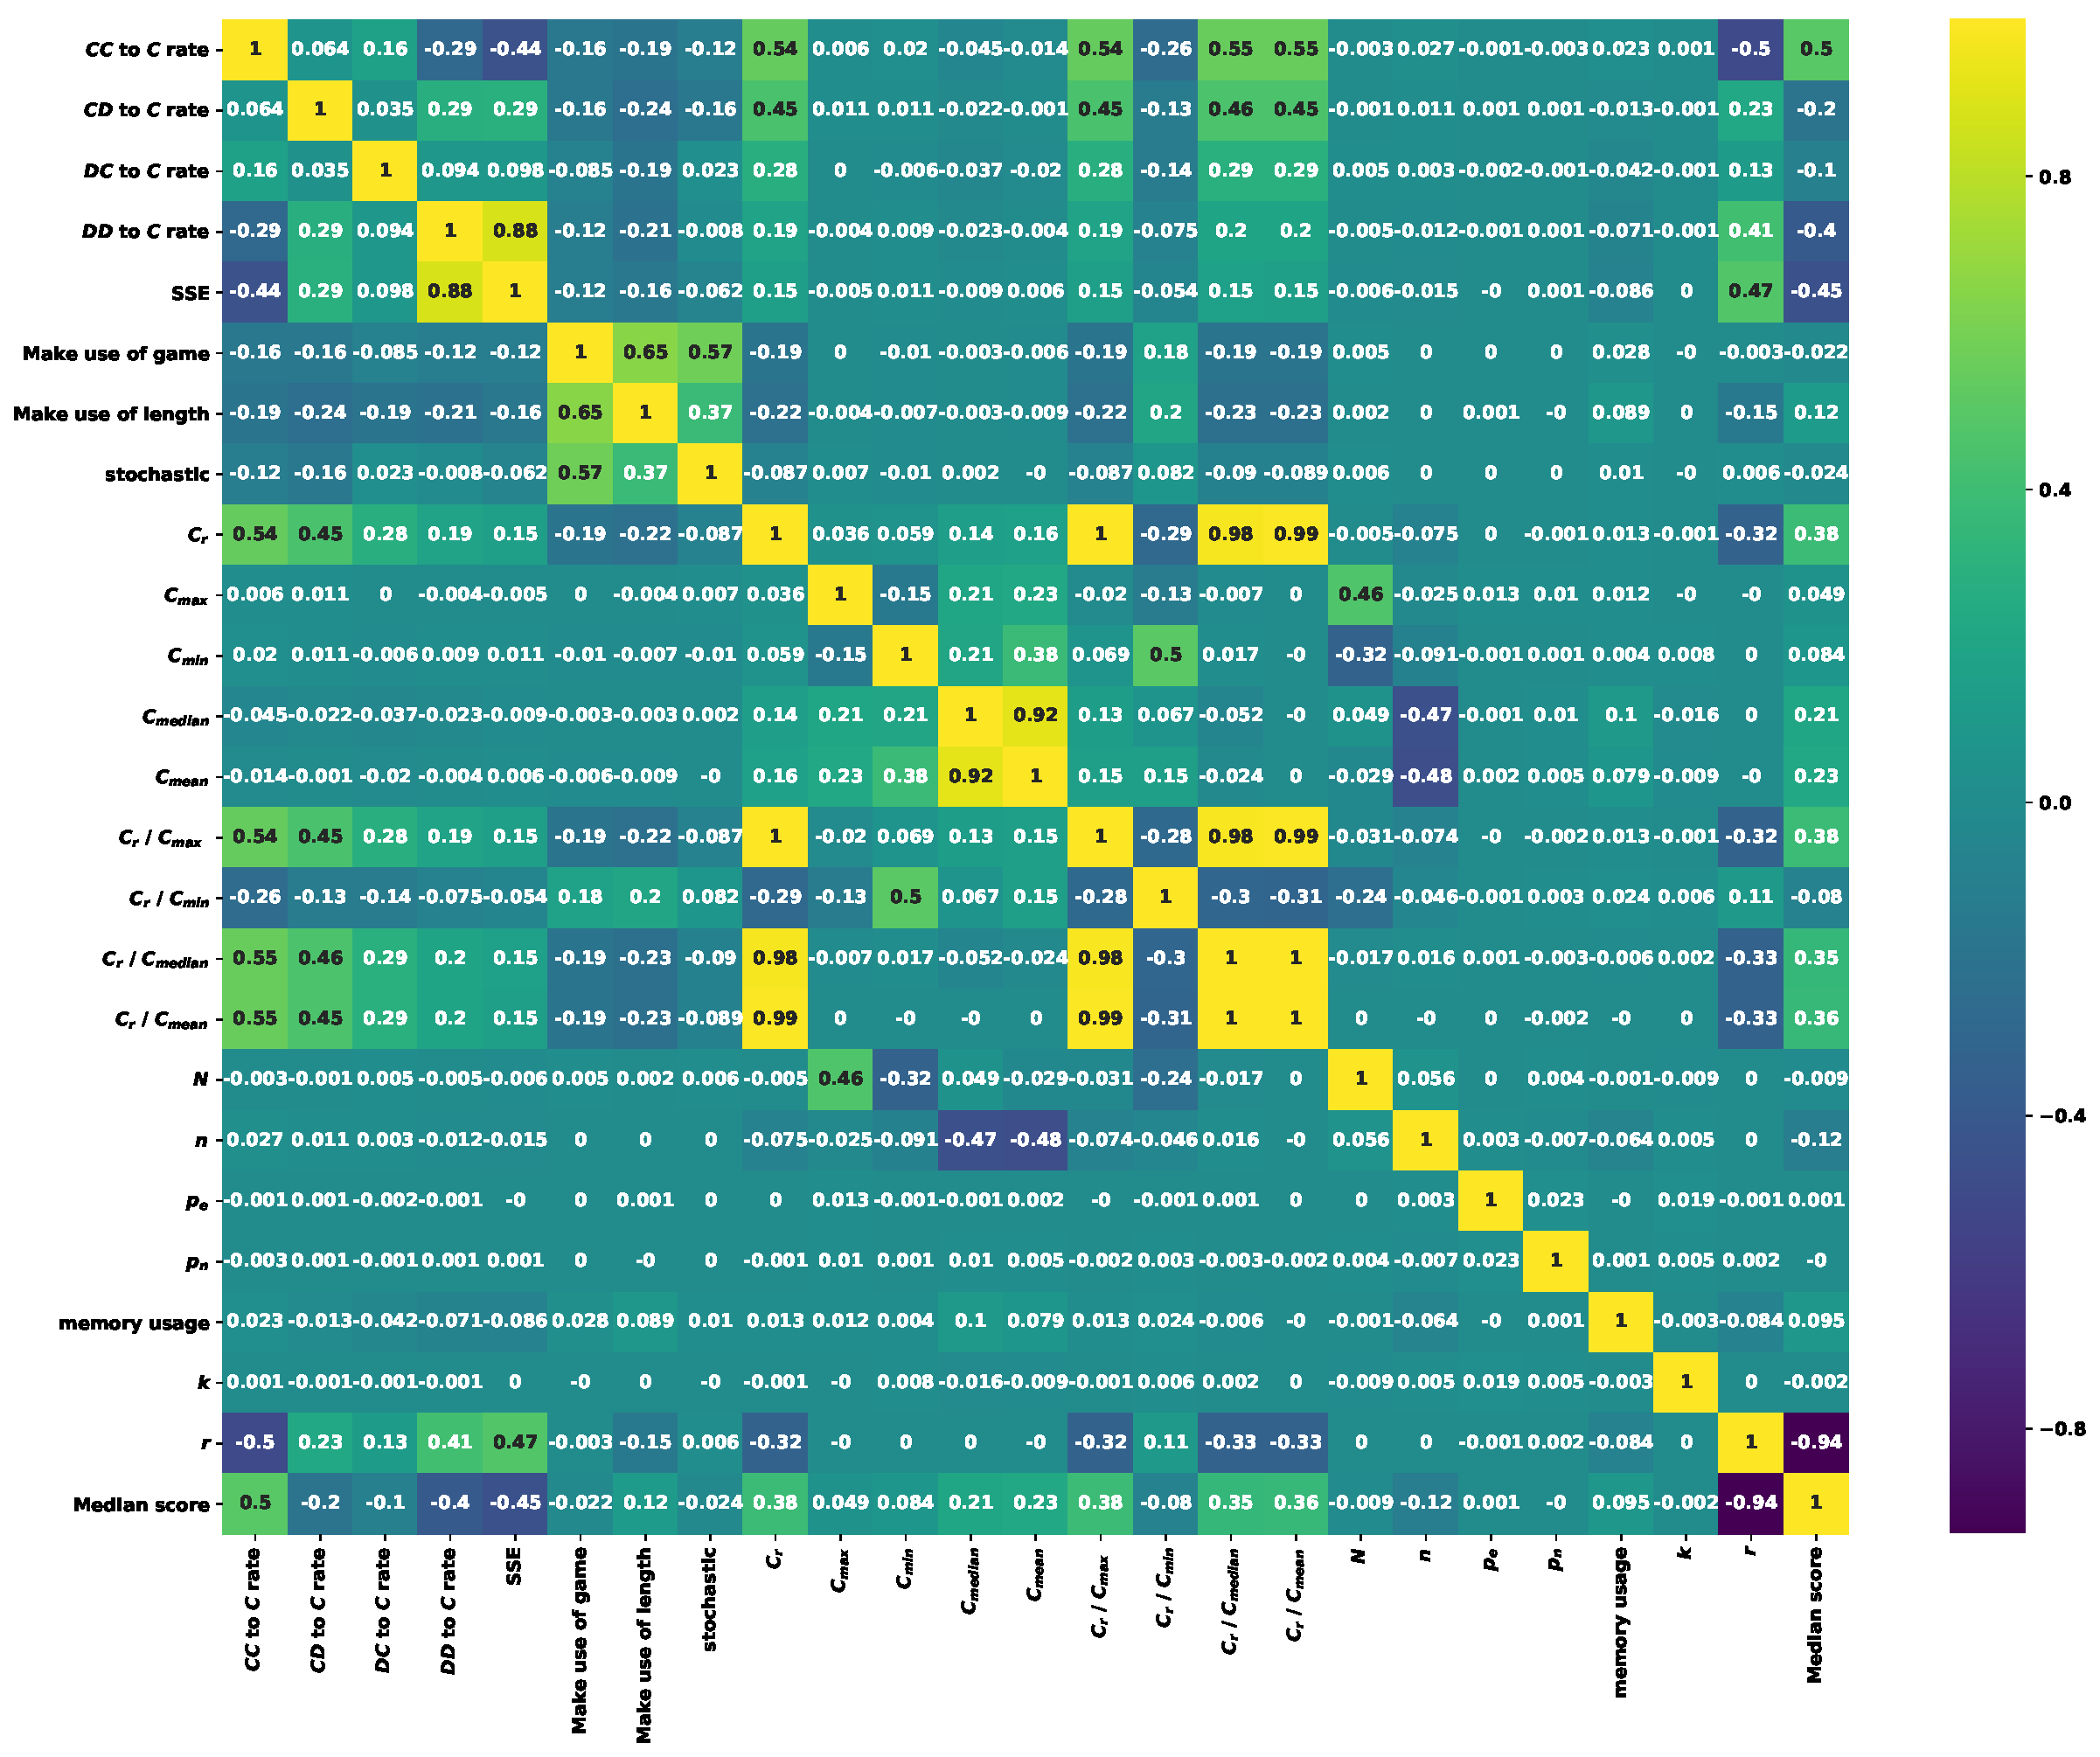
\includegraphics[width=.75\linewidth]{../images/merged_correlation_plot.pdf}
    \end{center}
    \caption{Correlation coefficients of features in Table~\ref{table:manual_features}
    for data set}
\end{figure}
\section{Evaluation based on clustering and random forest.}\label{app:clustering}

The final method to evaluate the features importance in a strategy's success
is a combination of a clustering task and a random forest algorithm.
Initially the performances are clustered into different clusters
based on them being successful or not. The performances are clustered into
successful and unsuccessful clusters based on 4 different approaches.
More specifically:

\begin{itemize}
    \item \textbf{Approach 1:} The performances are divided into two clusters based
    on whether their performance was in the top \(5\%\) of their respective tournaments.
    Thus, whether \(r\) was smaller or larger than 0.05.
    \item \textbf{Approach 2:} The performances are divided into two clusters based
    on whether their performance was in the top \(25\%\) of their respective tournaments.
    Thus, whether \(r\) was smaller or larger than 0.25.
    \item \textbf{Approach 3:} The performances are divided into two clusters based
    on whether their performance was in the top \(50\%\) of their respective tournaments.
    Thus, whether \(r\) was smaller or larger than 0.50.
    \item \textbf{Approach 4:} The performances are clustered based on their normalised rank and
    their median score by a \(k-\)means algorithm~\cite{Arthur2007}. The number of
    clusters is not deterministically chosen but it is based on the silhouette
    coefficients~\cite{Rousseeuw1987}.
\end{itemize}

Once the performances have been assigned to a cluster for each approach a
random forest algorithm~\cite{breiman2001} is applied. The problem is a supervised
problem where the random forest algorithm predicts the cluster to which a performance
has been assigned to using the features of Table~\ref{table:manual_features}.
The random
forest models are trained on a training set of 70\% of the tournaments results.
The accuracy of each model based on $R^2$ and the number of clusters for each
tournament type (because in the case of Approach 4 it is not
deterministically chosen) are given by Table~\ref{table:accuracy_random_forest}.
The out of the bag error (OOB)~\cite{hastie2005} has also been calculated. The
models fit well, and a high value of both the accuracy measures on the test data
and the OOB error indicate that the model is not over fitting.

\begin{table}[!htbp]
    \begin{center}
        \resizebox{.9\textwidth}{!}{
        \begin{tabular}{lccccc}
    \toprule
    Tournament type & Clustering Approach & Number of clusters & $R^2$ training data &  $R^2$ test data  & $R^2$ OOB score\\
    \midrule
    standard  & Approach 1  & 2 & 0.998831  & 0.987041    & 0.983708 \\
              & Approach 2  & 2 & 0.998643  & 0.978626    & 0.969202 \\
              & Approach 3  & 2 & 0.998417  & 0.985217    & 0.976538 \\
              & Approach 4  & 2 & 0.998794  & 0.990677    & 0.982959 \\
    \midrule
    noisy     & Approach 1  & 2 & 0.997786  & 0.972229    & 0.968332\\
              & Approach 2  & 2 & 0.997442  & 0.963254    & 0.955219\\
              & Approach 3  & 2 & 0.997152  & 0.953164    & 0.940528\\
              & Approach 4  & 3 & 0.996923  & 0.950728    & 0.935444\\
    \midrule
    probabilistic ending & Approach 1 & 2 & 0.997909   & 0.981490  & 0.978120 \\
                         & Approach 2 & 2 & 0.997883   & 0.973492  & 0.967150 \\
                         & Approach 3 & 2 & 0.990448   & 0.890068  & 0.875822 \\
                         & Approach 4 & 2 & 0.999636   & 0.995183  & 0.992809 \\
    \midrule
    noisy probabilistic ending & Approach 1  & 2 & 0.995347 & 0.957846   & 0.952353\\
                               & Approach 2  & 2 & 0.992813 & 0.909346   & 0.898613\\
                               & Approach 3  & 2 & 0.990579 & 0.824794   & 0.806540\\
                               & Approach 4  & 4 & 0.989465 & 0.841652   & 0.824052\\
    \midrule
    over \numberofalltournaments tournaments   & Approach 1 & 2 & 0.997271& 0.972914& 0.969198 \\
                                               & Approach 2 & 2 & 0.996323& 0.951194& 0.940563 \\
                                               & Approach 3 & 2 & 0.993707& 0.906941& 0.891532 \\
                                               & Approach 4 & 3 & 0.993556& 0.913335& 0.898453 \\
    \bottomrule
        \end{tabular}}
    \end{center}
    \caption{Accuracy metrics for random forest models.}
    \label{table:accuracy_random_forest}
\end{table}

The importance that the features of Table~\ref{table:manual_features} had on
each random forest model are given by Figures~\ref{fig:clustering_importance_standard},
\ref{fig:clustering_importance_noise},~\ref{fig:clustering_importance_probend},
\ref{fig:clustering_importance_probend_noise}
and~\ref{fig:clustering_importance_overall}. These show that the classifiers
stochastic, make use of game and make use of length have no significant effect,
and several of the features that are highlighted by the importance are inline with
the correlation results. Moreover, the smoothing parameter \(k\) appears to no
have a significant effect either. The most important features based on the
random forest analysis were $C_{r} / C_{median}$ and $C_r / C_{mean}$.

\begin{figure}[!htbp]
    \begin{subfigure}[t]{0.5\textwidth}
        \begin{center}
            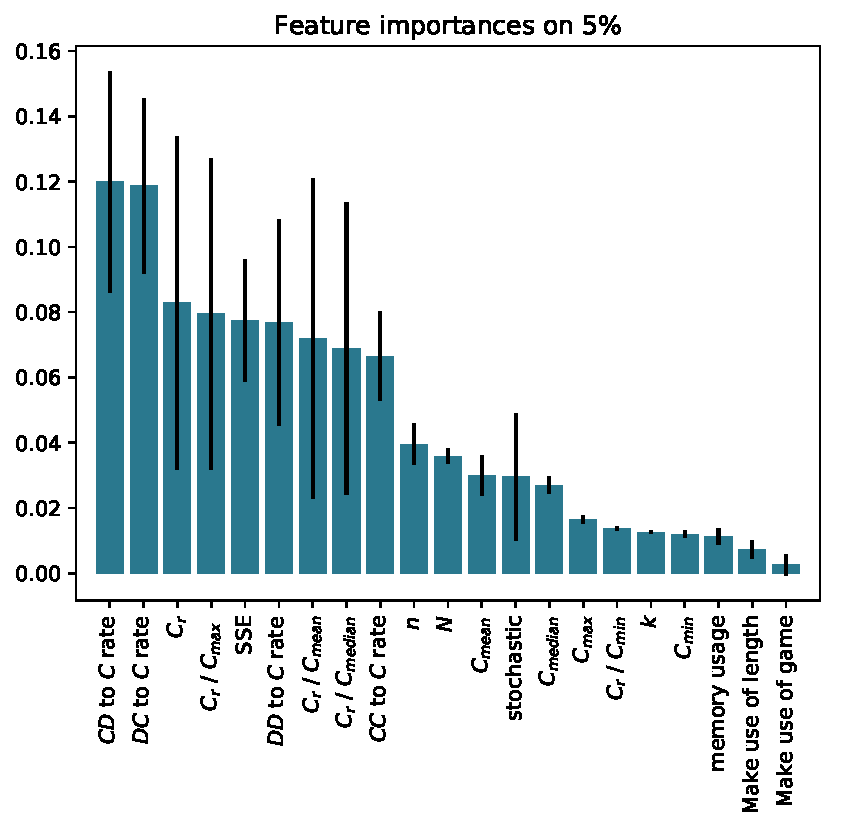
\includegraphics[width=.75\linewidth]{../new_output/standard/_feature_importance_bar_plot_cluster_on_0_05.pdf}
        \end{center}
        \caption{Importance of features for clusters on 5\% performance.}
    \end{subfigure}\hfill
    \begin{subfigure}[t]{0.5\textwidth}
        \begin{center}
            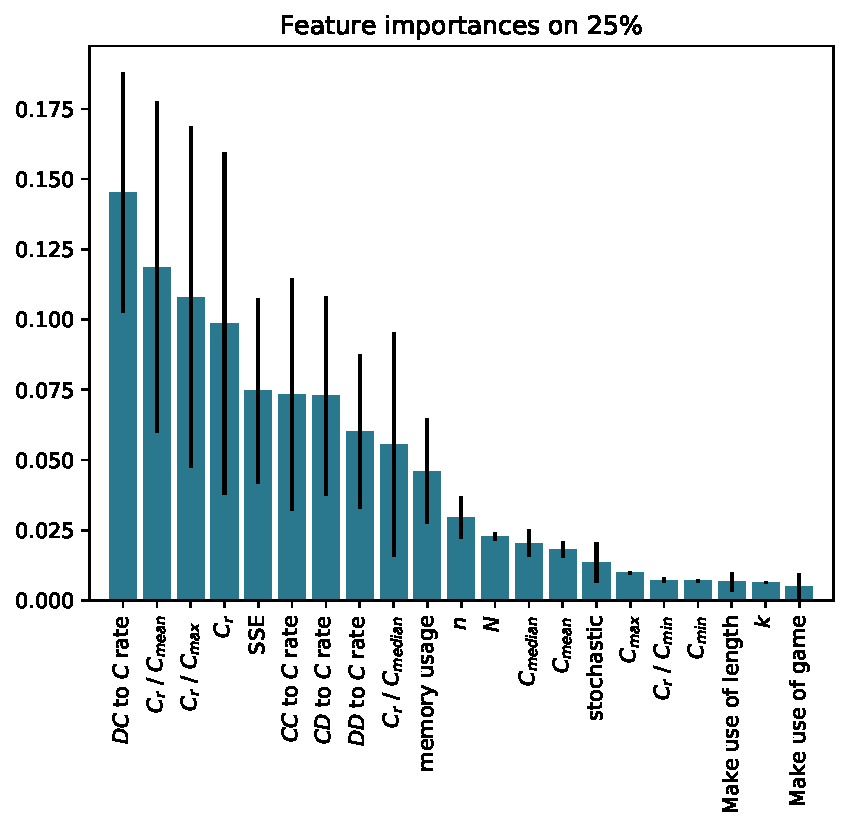
\includegraphics[width=.75\linewidth]{../new_output/standard/_feature_importance_bar_plot_cluster_on_0_25.pdf}
        \end{center}
        \caption{Importance of features for clusters on 25\% performance.}
    \end{subfigure}
    \begin{subfigure}[t]{0.5\textwidth}
        \begin{center}
            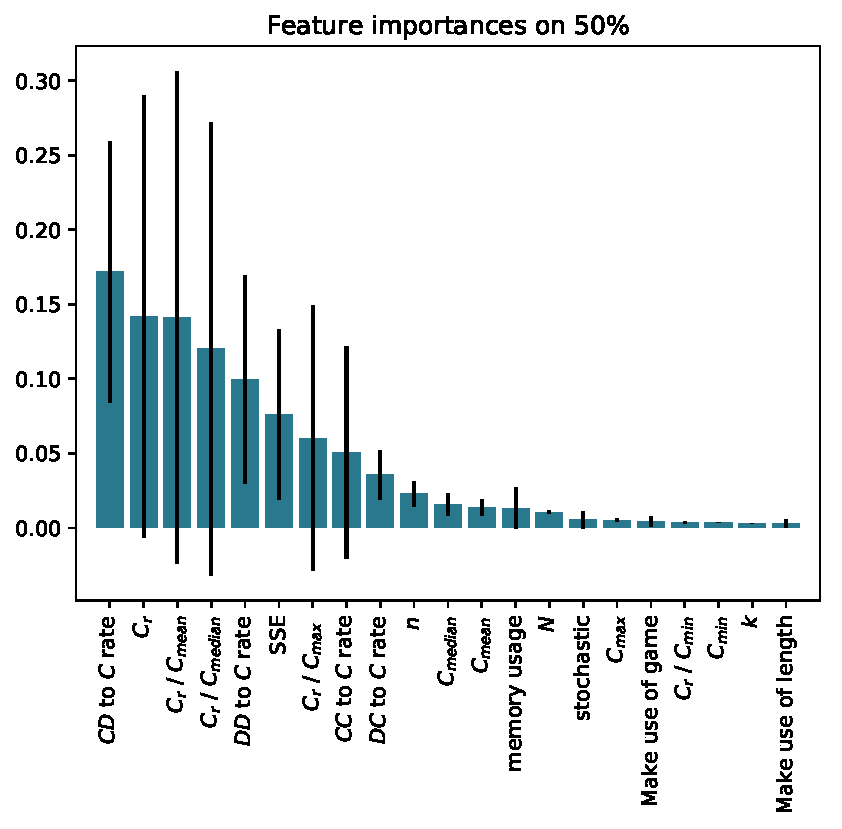
\includegraphics[width=.75\linewidth]{../new_output/standard/_feature_importance_bar_plot_cluster_on_0_5.pdf}
        \end{center}
        \caption{Importance of features for clusters on 50\% performance.}
    \end{subfigure}\hfill
    \begin{subfigure}[t]{0.5\textwidth}
        \begin{center}
            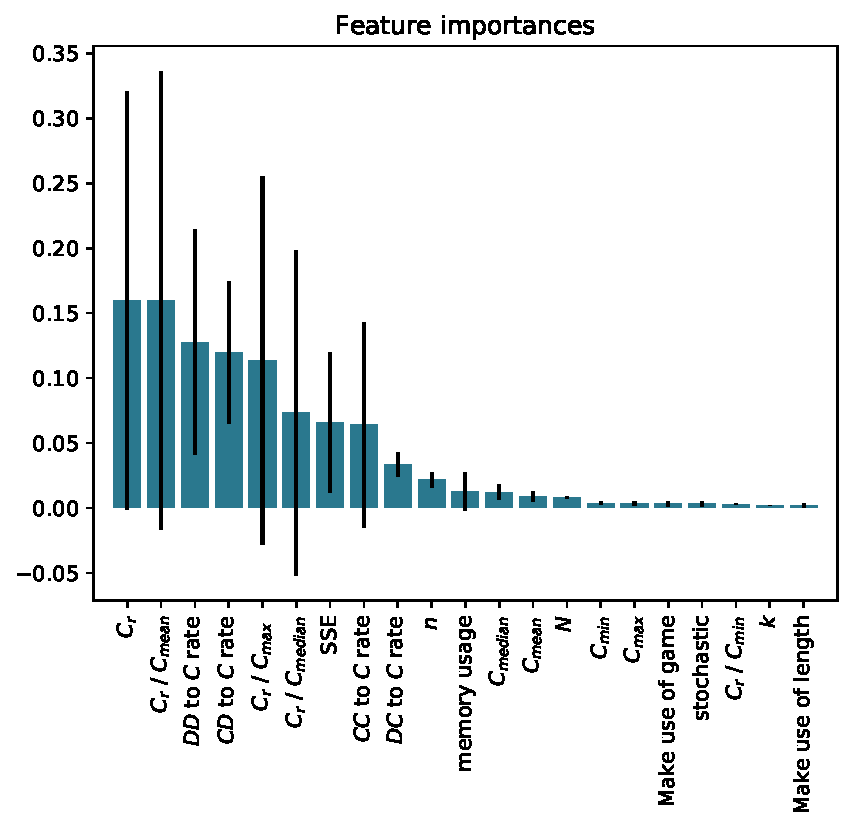
\includegraphics[width=.75\linewidth]{../k_means_output/standard/_feature_importance_bar_plot.pdf}
        \end{center}
        \caption{Importance of features for clusters based on \(k\)means algorithm.}
    \end{subfigure}
    \caption{Importance of features in standard tournaments for different
    clustering methods.}\label{fig:clustering_importance_standard}
\end{figure}

\begin{figure}[!htbp]
    \begin{subfigure}{0.5\textwidth}
        \begin{center}
            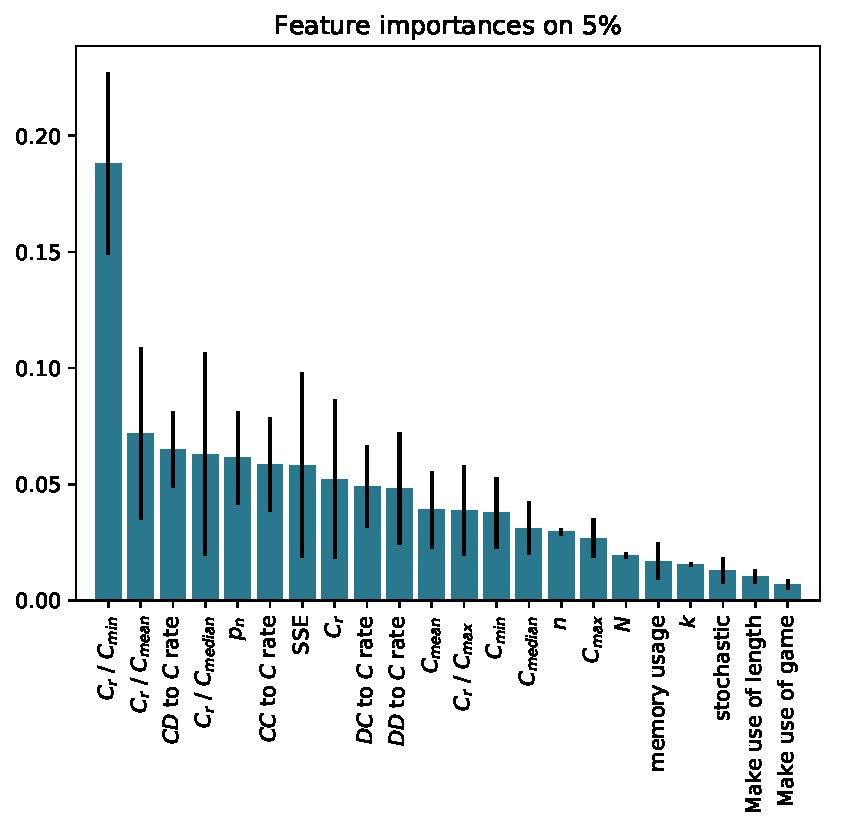
\includegraphics[width=.75\linewidth]{../new_output/noise/_feature_importance_bar_plot_cluster_on_0_05.pdf}
        \end{center}
        \caption{Importance of features for clusters on 5\% performance.}
    \end{subfigure}\hfill
    \begin{subfigure}{0.5\textwidth}
        \begin{center}
            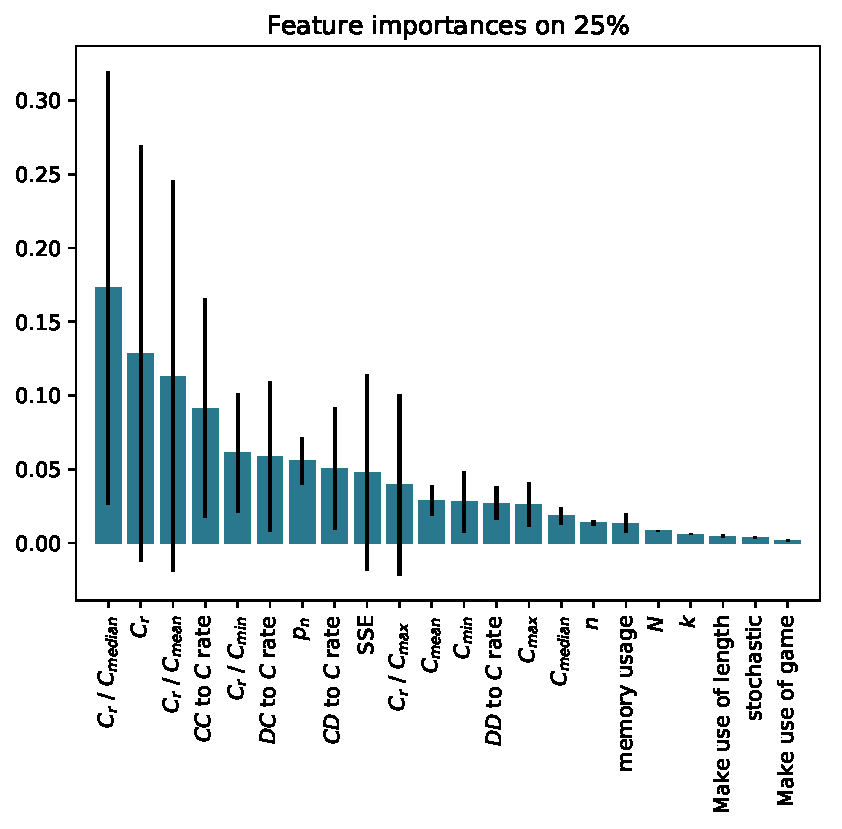
\includegraphics[width=.75\linewidth]{../new_output/noise/_feature_importance_bar_plot_cluster_on_0_25.pdf}
        \end{center}
        \caption{Importance of features for clusters on 25\% performance.}
    \end{subfigure}
    \begin{subfigure}{0.5\textwidth}
        \begin{center}
            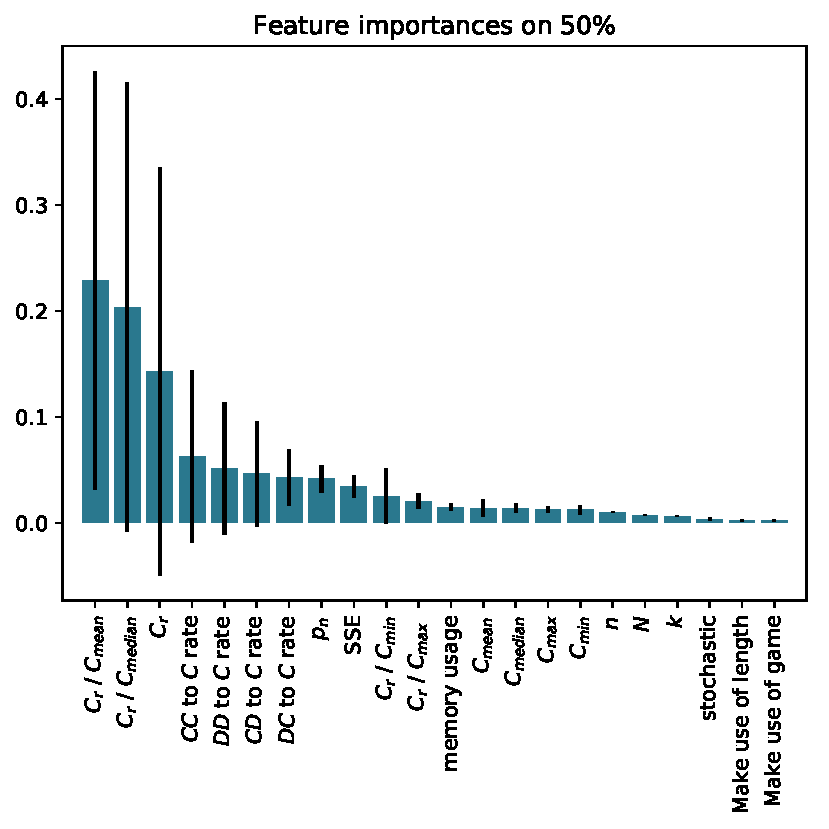
\includegraphics[width=.75\linewidth]{../new_output/noise/_feature_importance_bar_plot_cluster_on_0_5.pdf}
        \end{center}
        \caption{Importance of features for clusters on 50\% performance.}
    \end{subfigure}\hfill
    \begin{subfigure}{0.5\textwidth}
        \begin{center}
            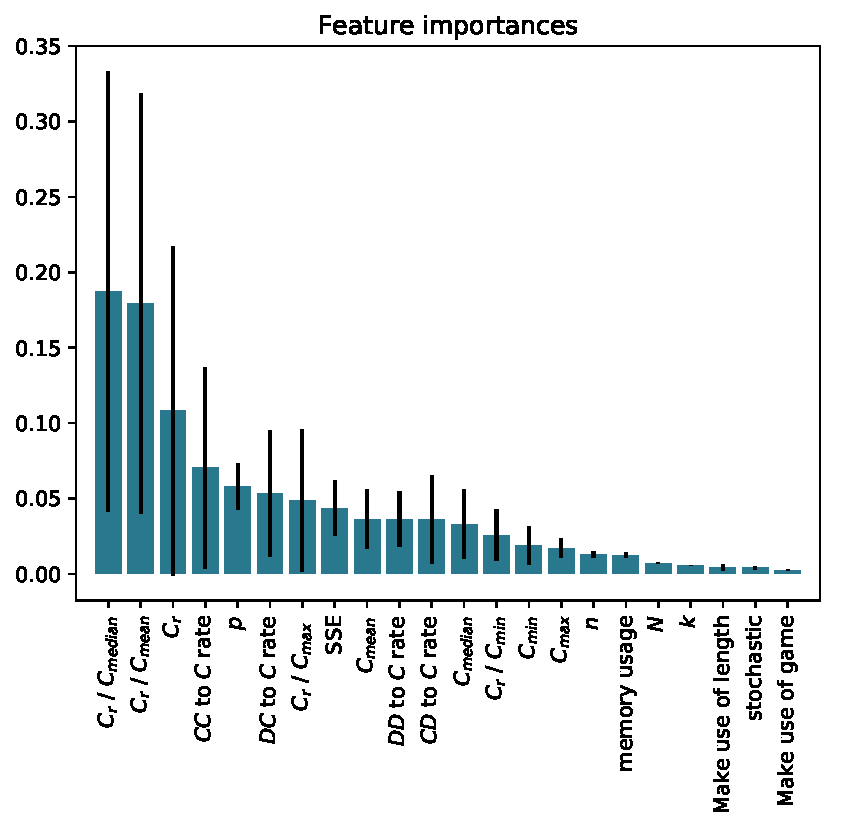
\includegraphics[width=.75\linewidth]{../k_means_output/noise/_feature_importance_bar_plot.pdf}
        \end{center}
        \caption{Importance of features for clusters based on \(k\)means algorithm.}
    \end{subfigure}
    \caption{Importance of features in noisy tournaments for different
    clustering methods.}\label{fig:clustering_importance_noise}
\end{figure}

\begin{figure}[!htbp]
    \begin{subfigure}[t]{0.5\textwidth}
        \begin{center}
            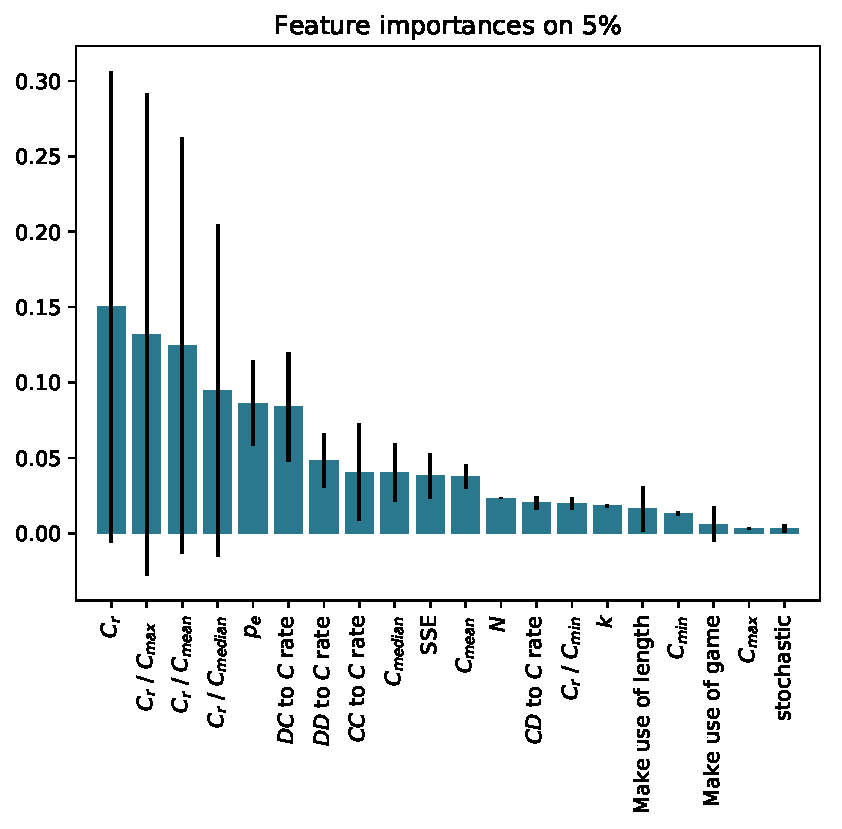
\includegraphics[width=.75\linewidth]{../new_output/probend/_feature_importance_bar_plot_cluster_on_0_05.pdf}
        \end{center}
        \caption{Importance of features for clusters on 5\% performance.}
    \end{subfigure}
    \begin{subfigure}[t]{0.5\textwidth}
        \begin{center}
            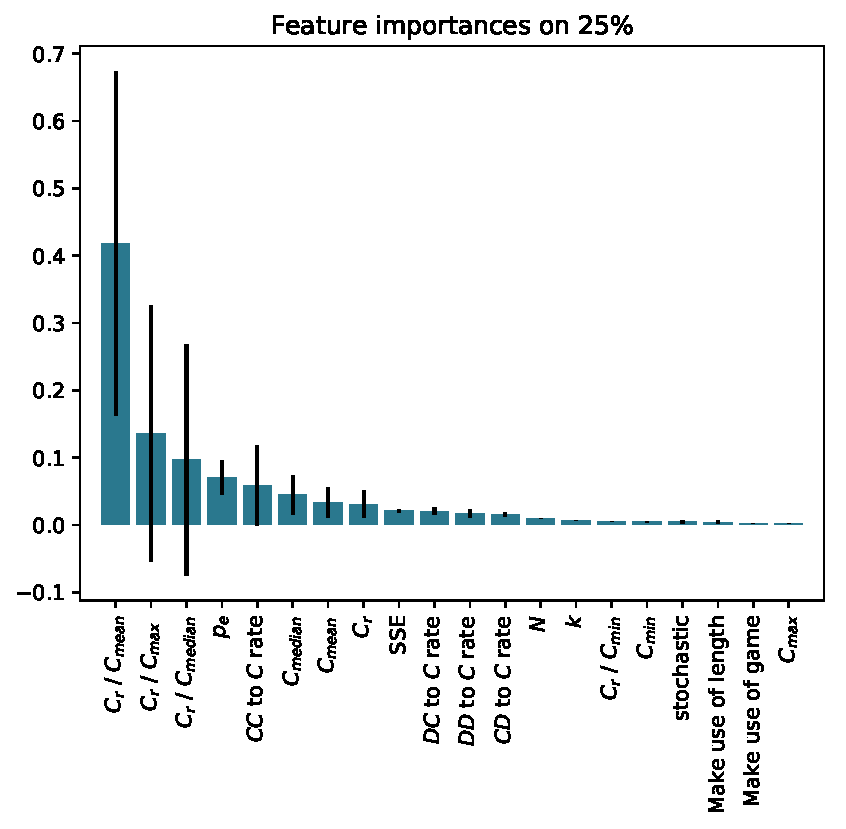
\includegraphics[width=.75\linewidth]{../new_output/probend/_feature_importance_bar_plot_cluster_on_0_25.pdf}
        \end{center}
        \caption{Importance of features for clusters on 25\% performance.}
    \end{subfigure}
    \begin{subfigure}[t]{0.5\textwidth}
        \begin{center}
            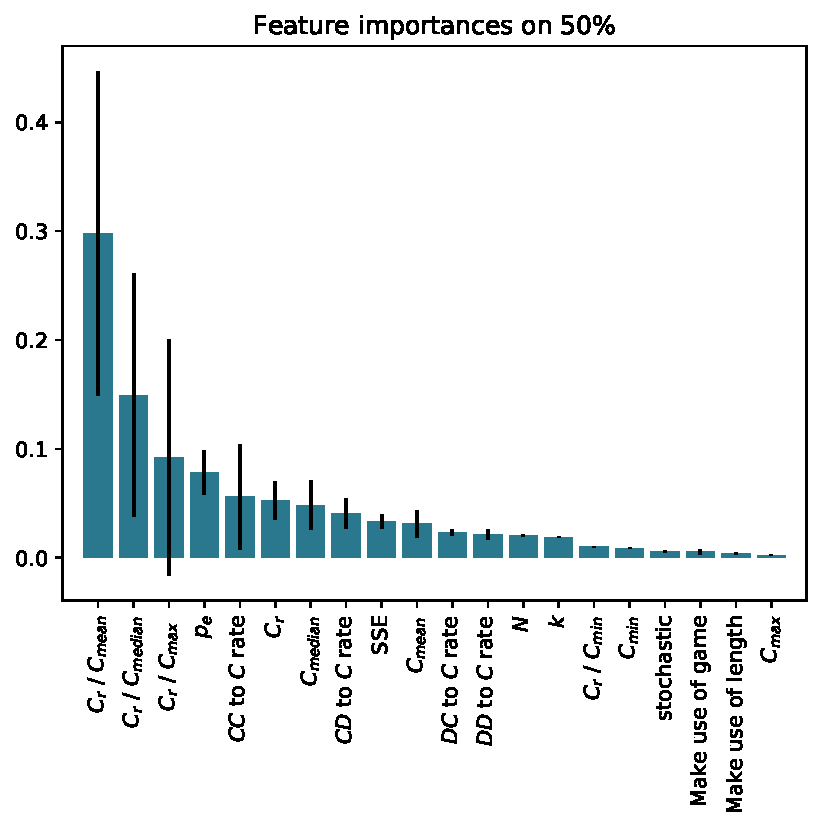
\includegraphics[width=.75\linewidth]{../new_output/probend/_feature_importance_bar_plot_cluster_on_0_5.pdf}
        \end{center}
        \caption{Importance of features for clusters on 50\% performance.}
    \end{subfigure}
    \begin{subfigure}[t]{0.5\textwidth}
        \begin{center}
            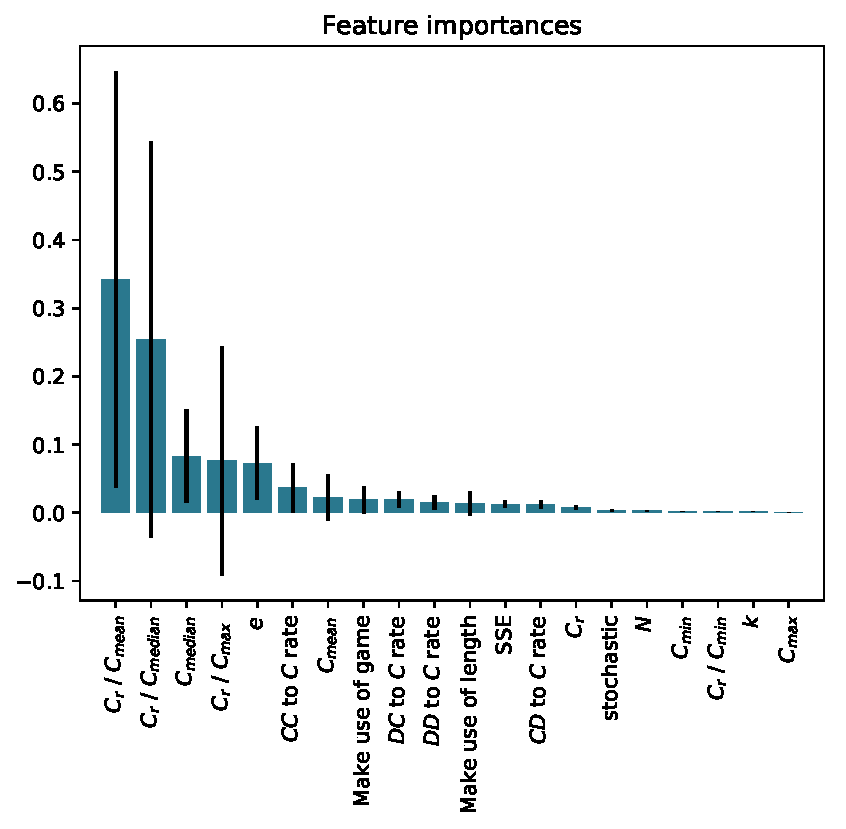
\includegraphics[width=.75\linewidth]{../k_means_output/probend/_feature_importance_bar_plot.pdf}
        \end{center}
        \caption{Importance of features for clusters based on \(k\)means algorithm.}
    \end{subfigure}
    \caption{Importance of features in probabilistic ending tournaments for different
    clustering methods.}\label{fig:clustering_importance_probend}
\end{figure}

\begin{figure}[!htbp]
    \begin{subfigure}[t]{0.5\textwidth}
        \begin{center}
            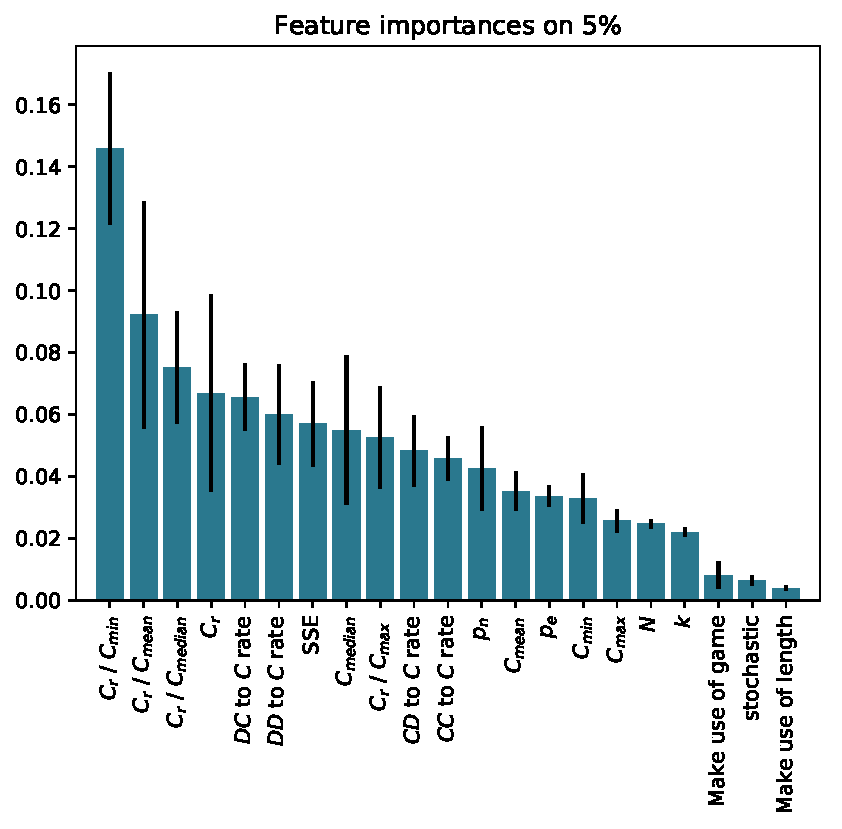
\includegraphics[width=.75\linewidth]{../new_output/probend_noise/_feature_importance_bar_plot_cluster_on_0_05.pdf}
        \end{center}
        \caption{Importance of features for clusters on 5\% performance.}
    \end{subfigure}
    \begin{subfigure}[t]{0.5\textwidth}
        \begin{center}
            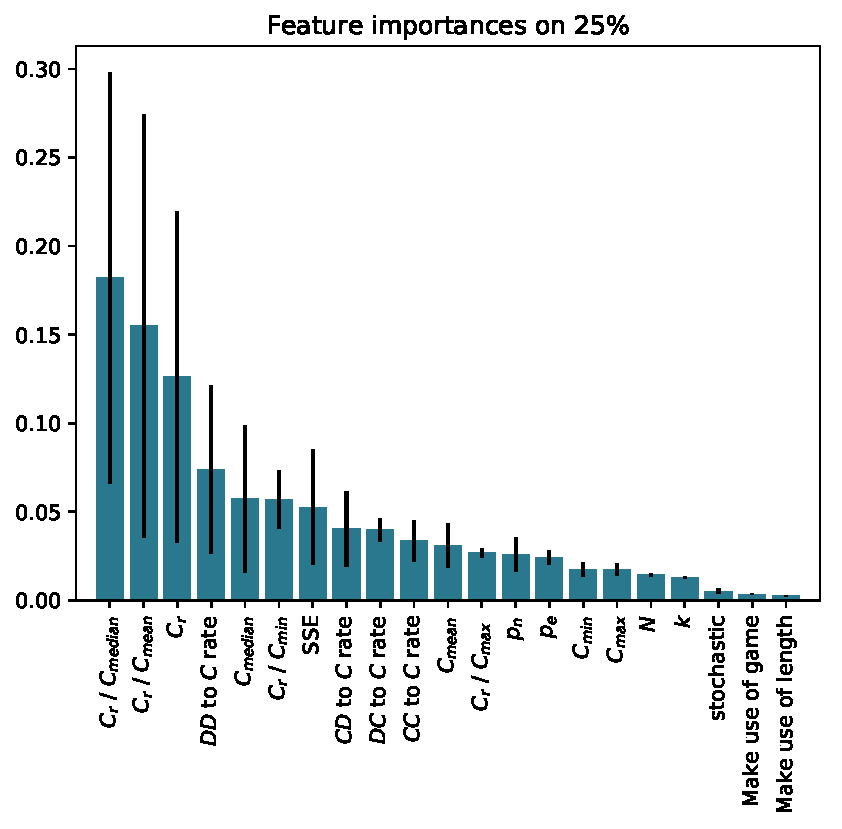
\includegraphics[width=.75\linewidth]{../new_output/probend_noise/_feature_importance_bar_plot_cluster_on_0_25.pdf}
        \end{center}
        \caption{Importance of features for clusters on 25\% performance.}
    \end{subfigure}
    \begin{subfigure}[t]{0.5\textwidth}
        \begin{center}
            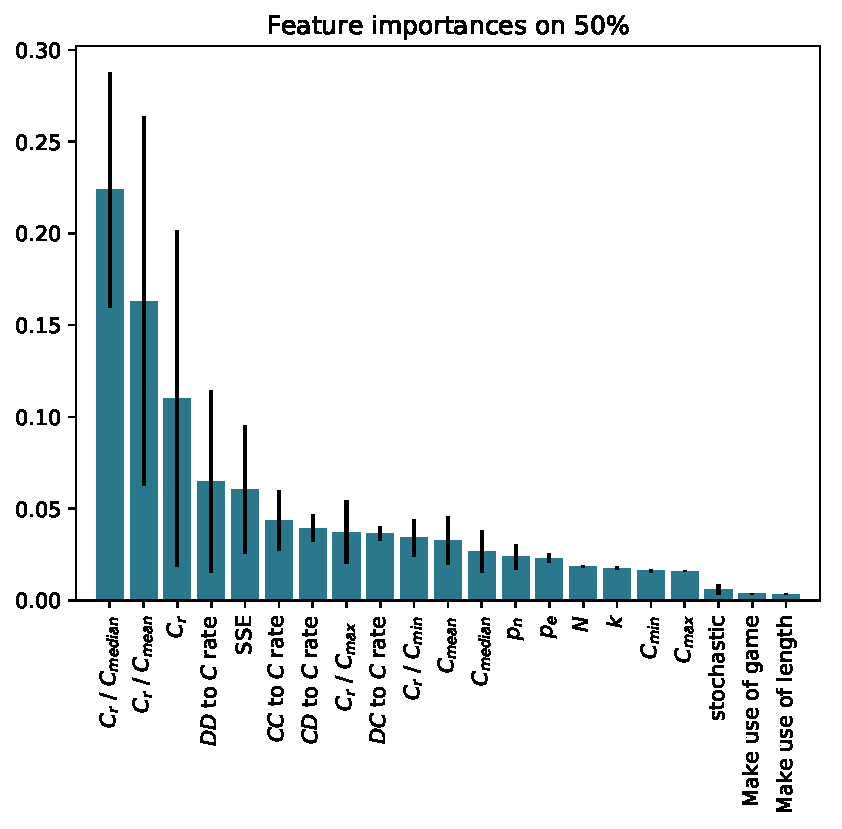
\includegraphics[width=.75\linewidth]{../new_output/probend_noise/_feature_importance_bar_plot_cluster_on_0_5.pdf}
        \end{center}
        \caption{Importance of features for clusters on 50\% performance.}
    \end{subfigure}
    \begin{subfigure}[t]{0.5\textwidth}
        \begin{center}
            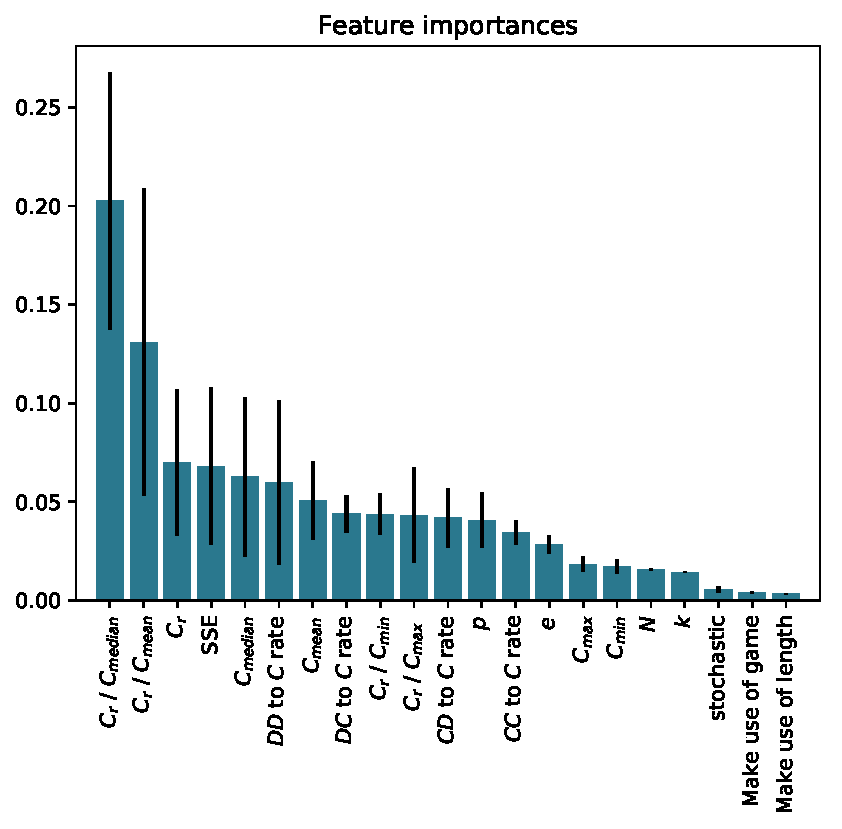
\includegraphics[width=.75\linewidth]{../k_means_output/probend_noise/_feature_importance_bar_plot.pdf}
        \end{center}
        \caption{Importance of features for clusters based on \(k\)means algorithm.}
    \end{subfigure}
    \caption{Importance of features in noisy probabilistic ending tournaments for different
    clustering methods.}\label{fig:clustering_importance_probend_noise}
\end{figure}

\begin{figure}[!htbp]
    \begin{subfigure}[t]{0.5\textwidth}
        \begin{center}
            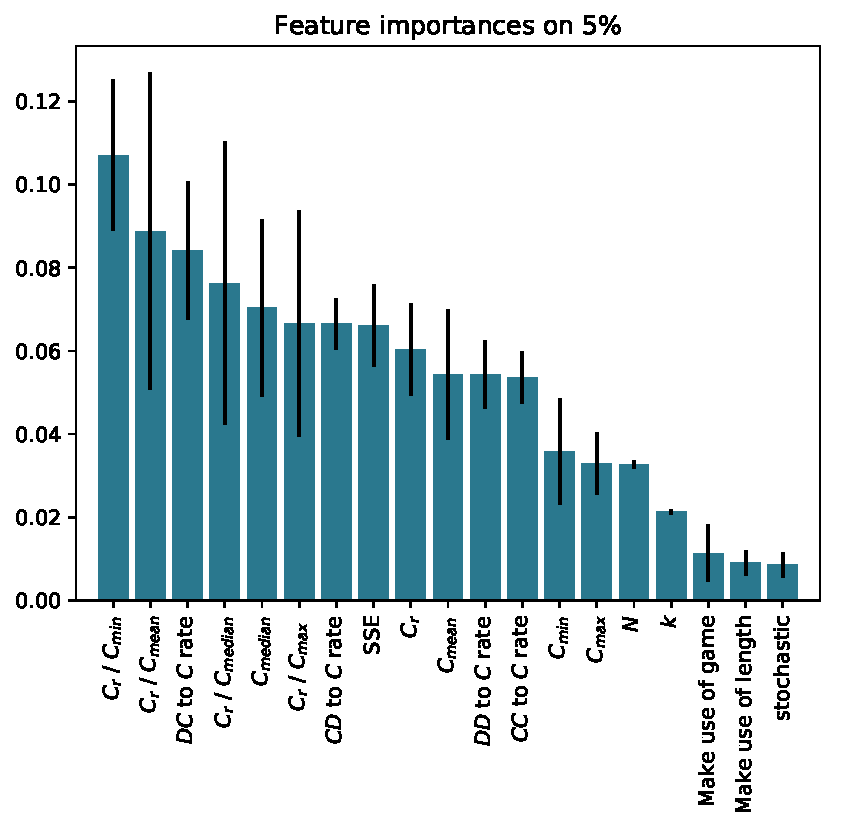
\includegraphics[width=.75\linewidth]{../new_output/merged/_feature_importance_bar_plot_cluster_on_0_05.pdf}
        \end{center}
        \caption{Importance of features for clusters on 5\% performance.}
    \end{subfigure}
    \begin{subfigure}[t]{0.5\textwidth}
        \begin{center}
            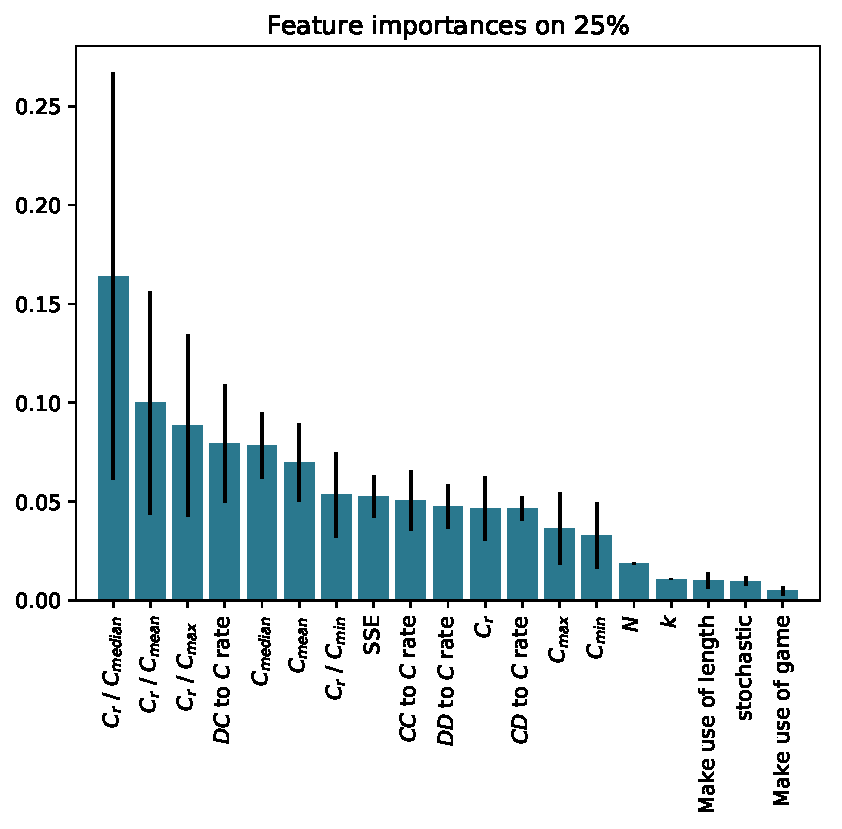
\includegraphics[width=.75\linewidth]{../new_output/merged/_feature_importance_bar_plot_cluster_on_0_25.pdf}
        \end{center}
        \caption{Importance of features for clusters on 25\% performance.}
    \end{subfigure}
    \begin{subfigure}[t]{0.5\textwidth}
        \begin{center}
            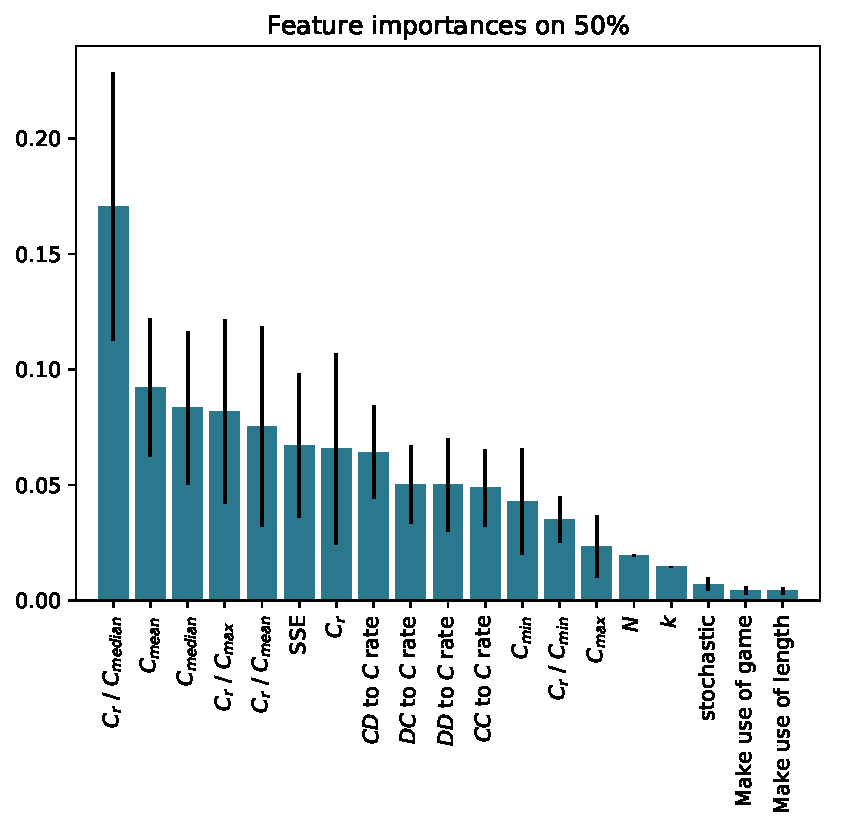
\includegraphics[width=.75\linewidth]{../new_output/merged/_feature_importance_bar_plot_cluster_on_0_5.pdf}
        \end{center}
        \caption{Importance of features for clusters on 50\% performance.}
    \end{subfigure}
    \begin{subfigure}[t]{0.5\textwidth}
        \begin{center}
            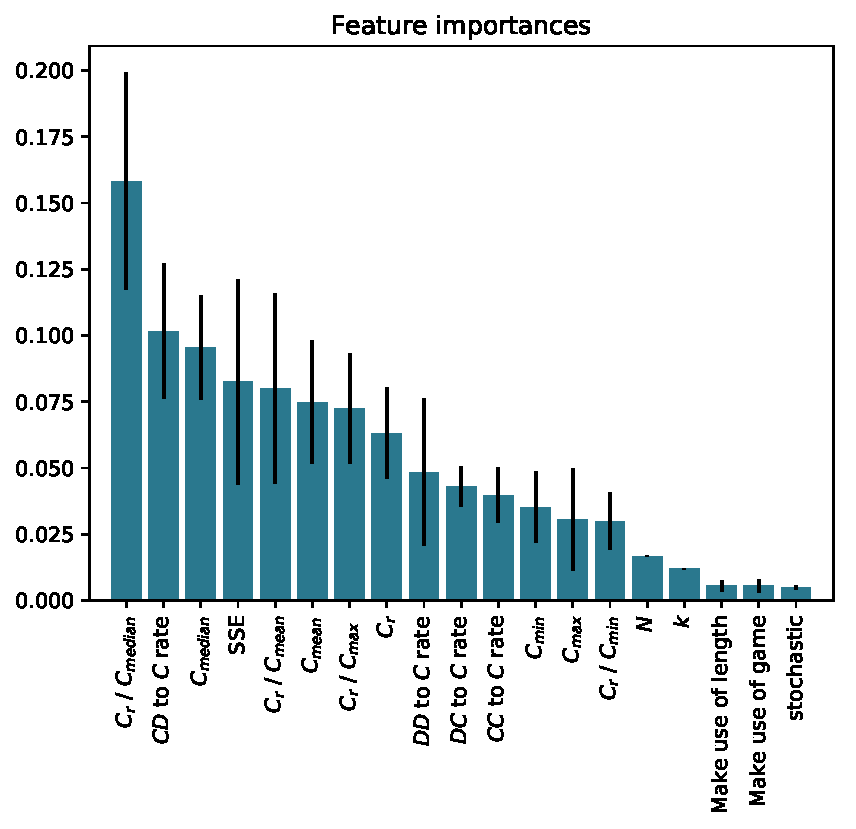
\includegraphics[width=.75\linewidth]{../k_means_output/merged/_feature_importance_bar_plot.pdf}
        \end{center}
        \caption{Importance of features for clusters based on \(k\)means algorithm.}
    \end{subfigure}
    \caption{Importance of features over all the tournaments for different
    clustering methods.}\label{fig:clustering_importance_overall}
\end{figure}
\section{Multivariate linear regression on median score}\label{app:regression_median_score}

A multivariate linear regression has also been fitted to model the relationship between
the features and the median score. The features included are given
by Table~\ref{table:linear_regression_on_median} alongside their corresponding \(p\) values
in the distinct tournaments and their regression coefficients.

\newcolumntype{g}{>{\columncolor{Gray}}c}
\begin{table}[h]
    \begin{center}
\resizebox{\textwidth}{!}{
\begin{tabular}{lggccggccgg}
    \toprule
    & \multicolumn{2}{g}{Standard} & \multicolumn{2}{c}{Noisy} & \multicolumn{2}{g}{Probabilistic ending} & \multicolumn{2}{c}{Noisy probabilistic ending} & \multicolumn{2}{g}{Overall}\\
    \midrule
    & \multicolumn{2}{g}{\(R\) adjusted: 0.576} & \multicolumn{2}{c}{\(R\) adjusted: 0.679} & \multicolumn{2}{g}{\(R\) adjusted: 0.816} & \multicolumn{2}{c}{\(R\) adjusted: 0.930} & \multicolumn{2}{g}{\(R\) adjusted: 0.318} \\
    {} &  Coefficient &  \(p\)-value &  Coefficient &  \(p\)-value &  Coefficient &  \(p\)-value &  Coefficient &  \(p\)-value &  Coefficient &  \(p\)-value \\
    \midrule
    $CC$ to $C$ rate   &  0.043 &  0.000 & -0.380 &  0.000 &  0.224 &  0.000 &  0.078 &    0.0 &  0.308 &    0.0 \\
    $CD$ to $C$ rate   & -0.325 &  0.000 &  0.124 &  0.000 &  0.060 &  0.000 &  0.073 &    0.0 & -0.014 &    0.0 \\
    $C_r$ / $C_{max}$  &      - &      - & -1.044 &  0.000 &      - &      - & -1.251 &    0.0 &      - &      - \\
    $C_r$ / $C_{mean}$ &  0.553 &  0.000 & -0.101 &  0.000 & -1.136 &  0.000 & -0.089 &    0.0 & -0.665 &    0.0 \\
    $C_{max}$          &  0.059 &  0.000 &      - &      - & -0.044 &  0.086 & -1.396 &    0.0 &      - &      - \\
    $C_{mean}$         &  1.837 &  0.000 &  3.078 &  0.000 &  1.506 &  0.000 &  3.645 &    0.0 &      - &      - \\
    $C_{min}$          &  0.156 &  0.000 &  1.528 &  0.000 &  0.311 &  0.000 &      - &      - &      - &      - \\
    $C_{min}$ / $C_r$  & -0.049 &  0.000 & -0.378 &  0.000 & -0.204 &  0.000 &      - &      - & -0.257 &    0.0 \\
    $DC$ to $C$ rate   & -0.204 &  0.000 &  0.074 &  0.000 &  0.066 &  0.000 &  0.066 &    0.0 &  0.007 &    0.0 \\
    $k$                & -0.000 &  0.853 & -0.000 &  0.987 &  0.000 &  0.008 &  0.000 &    0.0 &      - &      - \\
    $n$                & -0.000 &  0.000 &      - &      - &      - &      - &      - &      - &      - &      - \\
    $p_e$              &      - &      - &      - &      - &  0.025 &  0.000 & -0.095 &    0.0 &      - &      - \\
    $p_n$              &      - &      - &  0.124 &  0.000 &      - &      - &      - &      - &      - &      - \\
    SSE                & -0.294 &  0.000 & -0.319 &  0.000 &  0.055 &  0.000 &  0.010 &    0.0 & -0.015 &    0.0 \\
    constant           &  0.925 &  0.000 &  1.536 &  0.000 &  2.466 &  0.000 &  2.299 &    0.0 &  2.924 &    0.0 \\
    memory usage       &  0.010 &  0.000 & -0.004 &  0.000 &      - &      - &      - &      - &      - &      - \\
    \bottomrule
\end{tabular}}
\end{center}
\caption{Results of multivariate linear regressions with the median score as the dependent variable.
\(R\) squared is reported for each model.}
\label{table:linear_regression_on_median}
\end{table}
\section{List of strategies}\label{app:list_of_players}

The strategies used in this study which are from Axelrod-Python library version 3.0.0.

\begin{multicols}{3}
	\begin{enumerate}
		\item $\phi$~\cite{axelrodproject}
\item $\pi$~\cite{axelrodproject}
\item $e$~\cite{axelrodproject}
\item ALLCorALLD \cite{axelrodproject}
\item Adaptive~\cite{Li2011}
\item Adaptive Pavlov 2006~\cite{kendall2007iterated}
\item Adaptive Pavlov 2011~\cite{Li2011}
\item Adaptive Tit For Tat: 0.5~\cite{Tzafestas2000}
\item Aggravater~\cite{axelrodproject}
\item Alexei~\cite{lesswrong}
\item Alternator~\cite{Axelrod1981, Mittal2009}
\item Alternator Hunter~\cite{axelrodproject}
\item Anti Tit For Tat~\cite{Hilbe2013}
\item AntiCycler~\cite{axelrodproject}
\item Appeaser~\cite{axelrodproject}
\item Arrogant QLearner~\cite{axelrodproject}
\item Average Copier~\cite{axelrodproject}
\item Backstabber~\cite{axelrodproject}
\item Better and Better~\cite{prison}
\item Bully~\cite{Nachbar1992}
\item Calculator~\cite{prison}
\item Cautious QLearner~\cite{axelrodproject}
\item Champion~\cite{Axelrod1980b}
\item CollectiveStrategy~\cite{Li2009}
\item Contrite Tit For Tat~\cite{Axelrod1995}
\item Cooperator~\cite{Axelrod1981, Mittal2009, Press2012}
\item Cooperator Hunter~\cite{axelrodproject}
\item Cycle Hunter~\cite{axelrodproject}
\item Cycler CCCCCD~\cite{axelrodproject}
\item Cycler CCCD~\cite{axelrodproject}
\item Cycler CCCDCD~\cite{axelrodproject}
\item Cycler CCD~\cite{Mittal2009}
\item Cycler DC~\cite{axelrodproject}
\item Cycler DDC~\cite{Mittal2009}
\item DBS~\cite{Au2006}
\item Davis~\cite{Axelrod1980a}
\item Defector~\cite{Axelrod1981, Mittal2009, Press2012}
\item Defector Hunter~\cite{axelrodproject}
\item Double Crosser~\cite{axelrodproject}
\item Desperate \cite{Van2015}
\item DoubleResurrection~\cite{Eckhart2015}
\item Doubler~\cite{prison}
\item Dynamic Two Tits For Tat~\cite{axelrodproject}
\item EasyGo~\cite{Li2011, prison}
\item Eatherley~\cite{Axelrod1980b}
\item Eventual Cycle Hunter~\cite{axelrodproject}
\item Evolved ANN~\cite{axelrodproject}
\item Evolved ANN 5~\cite{axelrodproject}
\item Evolved ANN 5 Noise 05~\cite{axelrodproject}
\item Evolved FSM 16~\cite{axelrodproject}
\item Evolved FSM 16 Noise 05~\cite{axelrodproject}
\item Evolved FSM 4~\cite{axelrodproject}
\item Evolved HMM 5~\cite{axelrodproject}
\item EvolvedLookerUp1 1 1~\cite{axelrodproject}
\item EvolvedLookerUp2 2 2~\cite{axelrodproject}
\item Eugine Nier~\cite{lesswrong}
\item Feld~\cite{Axelrod1980a}
\item Firm But Fair~\cite{Frean1994}
\item Fool Me Forever~\cite{axelrodproject}
\item Fool Me Once~\cite{axelrodproject}
\item Forgetful Fool Me Once~\cite{axelrodproject}
\item Forgetful Grudger~\cite{axelrodproject}
\item Forgiver~\cite{axelrodproject}
\item Forgiving Tit For Tat~\cite{axelrodproject}
\item Fortress3~\cite{Ashlock2006}
\item Fortress4~\cite{Ashlock2006}
\item GTFT \cite{Gaudesi2016, Nowak1993}
\item General Soft Grudger~\cite{axelrodproject}
\item Gradual~\cite{Beaufils1997}
\item Gradual Killer~\cite{prison}
\item Grofman\cite{Axelrod1980a}
\item Grudger~\cite{Axelrod1980a, Banks1990, Beaufils1997, Van2015, Li2011}
\item GrudgerAlternator~\cite{prison}
\item Grumpy~\cite{axelrodproject}
\item Handshake~\cite{Robson1990}
\item Hard Go By Majority~\cite{Mittal2009}
\item Hard Go By Majority: 10~\cite{axelrodproject}
\item Hard Go By Majority: 20~\cite{axelrodproject}
\item Hard Go By Majority: 40~\cite{axelrodproject}
\item Hard Go By Majority: 5~\cite{axelrodproject}
\item Hard Prober~\cite{prison}
\item Hard Tit For 2 Tats~\cite{Stewart2012}
\item Hard Tit For Tat~\cite{PD2017}
\item Hesitant QLearner\cite{axelrodproject}
\item Hopeless~\cite{Van2015}
\item Inverse~\cite{axelrodproject}
\item Inverse Punisher~\cite{axelrodproject}
\item Joss~\cite{Axelrod1980a, Stewart2012}
\item Knowledgeable Worse and Worse~\cite{axelrodproject}
\item Level Punisher~\cite{Eckhart2015}
\item Limited Retaliate 2~\cite{axelrodproject}
\item Limited Retaliate 3~\cite{axelrodproject}
\item Limited Retaliate~\cite{axelrodproject}
\item MEM2~\cite{Li2014}
\item Math Constant Hunter~\cite{axelrodproject}
\item Meta Hunter Aggressive~\cite{axelrodproject}
\item Meta Hunter~\cite{axelrodproject}
\item Meta Majority~\cite{axelrodproject}
\item Meta Majority Finite Memory~\cite{axelrodproject}
\item Meta Majority Long Memory~\cite{axelrodproject}
\item Meta Majority Memory One~\cite{axelrodproject}
\item Meta Minority~\cite{axelrodproject}
\item Meta Mixer~\cite{axelrodproject}
\item Meta Winner~\cite{axelrodproject}
\item Meta Winner Deterministic~\cite{axelrodproject}
\item Meta Winner Ensemble~\cite{axelrodproject}
\item Meta Winner Finite Memory~\cite{axelrodproject}
\item Meta Winner Long Memory~\cite{axelrodproject}
\item Meta Winner Memory One~\cite{axelrodproject}
\item Meta Winner Stochastic~\cite{axelrodproject}
\item NMWE Deterministic~\cite{axelrodproject}
\item NMWE Finite Memory~\cite{axelrodproject}
\item NMWE Long Memory~\cite{axelrodproject}
\item NMWE Memory One~\cite{axelrodproject}
\item NMWE Stochastic~\cite{axelrodproject}
\item Naive Prober~\cite{Li2011}
\item Negation~\cite{PD2017}
\item Nice Average Copier~\cite{axelrodproject}
\item Nice Meta Winner~\cite{axelrodproject}
\item Nice Meta Winner Ensemble~\cite{axelrodproject}
\item Nydegger~\cite{Axelrod1980a}
\item Omega TFT~\cite{kendall2007iterated}
\item Once Bitten~\cite{axelrodproject}
\item Opposite Grudger~\cite{axelrodproject}
\item PSO Gambler 1 1 1~\cite{axelrodproject}
\item PSO Gambler 2 2 2~\cite{axelrodproject}
\item PSO Gambler 2 2 2 Noise 05~\cite{axelrodproject}
\item PSO Gambler Mem1 \cite{axelrodproject}
\item Predator~\cite{Ashlock2006}
\item Prober~\cite{Li2011}
\item Prober 2~\cite{prison}
\item Prober 3~\cite{prison}
\item Prober 4~\cite{prison}
\item Pun1~\cite{Ashlock2006}
\item Punisher~\cite{axelrodproject}
\item Raider~\cite{Ashlock2014}
\item Random Hunter~\cite{axelrodproject}
\item Random: 0.5~\cite{Axelrod1980a, Tzafestas2000}
\item Remorseful Prober~\cite{Li2011}
\item Resurrection~\cite{Eckhart2015}
\item Retaliate 2~\cite{axelrodproject}
\item Retaliate 3~\cite{axelrodproject}
\item Retaliate~\cite{axelrodproject}
\item Revised Downing~\cite{Axelrod1980a}
\item Ripoff~\cite{Ashlock2008}
\item Risky QLearner~\cite{axelrodproject}
\item SelfSteem~\cite{Andre2013}
\item ShortMem ~\cite{Andre2013}
\item Shubik~\cite{Axelrod1980a}
\item Slow Tit For Two Tats~\cite{axelrodproject}
\item Slow Tit For Two Tats 2~\cite{prison}
\item Sneaky Tit For Tat~\cite{axelrodproject}
\item Soft Go By Majority~\cite{Axelrod1981, Mittal2009}
\item Soft Go By Majority 10~\cite{axelrodproject}
\item Soft Go By Majority 20~\cite{axelrodproject}
\item Soft Go By Majority 40~\cite{axelrodproject}
\item Soft Go By Majority 5~\cite{axelrodproject}
\item Soft Grudger~\cite{Li2011}
\item Soft Joss~\cite{prison}
\item SolutionB1~\cite{Ashlock2015}
\item SolutionB5~\cite{Ashlock2015}
\item Spiteful Tit For Tat~\cite{prison}
\item Stalker~\cite{Carvalho2013}
\item Stein and Rapoport~\cite{Axelrod1980a}
\item Stochastic Cooperator~\cite{Adami2013}
\item Stochastic WSLS~\cite{axelrodproject}
\item Suspicious Tit For Tat~\cite{Beaufils1997, Hilbe2013}
\item TF1~\cite{axelrodproject}
\item TF2~\cite{axelrodproject}
\item TF3~\cite{axelrodproject}
\item Tester~\cite{Axelrod1980b}
\item ThueMorse~\cite{axelrodproject}
\item ThueMorseInverse~\cite{axelrodproject}
\item Thumper~\cite{Ashlock2008}
\item Tit For 2 Tats (\textbf{Tf2T})~\cite{Axelrod1981}
\item Tit For Tat (\textbf{TFT})~\cite{Axelrod1980a}
\item Tricky Cooperator~\cite{axelrodproject}
\item Tricky Defector~\cite{axelrodproject}
\item Tullock~\cite{Axelrod1980a}
\item Two Tits For Tat (\textbf{2TFT})~\cite{Axelrod1981}
\item VeryBad~\cite{Andre2013}
\item Willing \cite{Van2015}
\item Win-Shift Lose-Stay (\textbf{WShLSt})~\cite{Li2011}
\item Win-Stay Lose-Shift (\textbf{WSLS})~\cite{Kraines1989, Nowak1993, Stewart2012}
\item Winner12~\cite{mathieu2017}
\item Winner21~\cite{mathieu2017}
\item Worse and Worse\cite{prison}
\item Worse and Worse 2\cite{prison}
\item Worse and Worse 3\cite{prison}
\item ZD-Extort-2 v2~\cite{Kuhn2017}
\item ZD-Extort-2~\cite{Stewart2012}
\item ZD-Extort-4~\cite{axelrodproject}
\item ZD-GEN-2~\cite{Kuhn2017}
\item ZD-GTFT-2~\cite{Stewart2012}
\item ZD-SET-2~\cite{Kuhn2017}
	\end{enumerate}
\end{multicols}

\end{document}
